%===================================================
%================== DOCUMENT CLASS
%===================================================
\documentclass[runningheads,11pt,a4paper,english,llncs]{Misc/llncs}

%===================================================
%================== PACKAGES
%===================================================
%------------------------------------------------------------------------
% TeX and LaTeX macros
%------------------------------------------------------------------------
%
% In math formulas we use italic instead of mathitalic
%
\makeatletter
% ~ gives a \; space in math mode
\def~{\ifmmode\;\else\penalty\@M\ \fi}
%  Italic in mathematical formulas
\def\@setmcodes#1#2#3{{\count0=#1 \count1=#3
  \loop \global\mathcode\count0=\count1 \ifnum \count0<#2
  \advance\count0 by1 \advance\count1 by1 \repeat}}
\DeclareSymbolFont{italic}{OT1}{\rmdefault}{m}{it}
\let\mathit\undefined
\DeclareSymbolFontAlphabet{\mathit}{italic}
\edef\@tempa{\hexnumber@\symitalic}
\@setmcodes{`A}{`Z}{"7\@tempa41}
\@setmcodes{`a}{`z}{"7\@tempa61}
\makeatother
%
% \begin{asm} ... \end{asm}
%
\newdimen\asmindent     
\asmindent=\parindent
\newcount\asmi
\def\inc{\global\advance\asmi by 1}
\def\dec{\global\advance\asmi by-1}
\def\nl{{}$\par\hangindent\asmi em
  \noindent\kern\asmi em\ignorespaces$} 
\def\asmskip{{}$\par\smallskip\hangindent\asmi em
  \noindent\kern\asmi em\ignorespaces$} 
\def\asm{\global\asmi=0 
%%%%%%%%%%%%%% added by Paolo:
\parskip=0pt
%%%%%%%%%%%%%%%%%%%%%%%
 \def\+{\inc\nl}
 \def\-{\dec\nl}
 \def\\{\nl}
 \begin{trivlist}\item[]\leftskip=\asmindent\relax$}
\def\endasm{$\end{trivlist}}
%\mathindent=\asmindent
%
% \begin{asmarray}
%    f(s_1) & := t_1 \\
%    f(s_2) & := t_2 
% \end{asmarray}
%
\def\asmarray{\begin{array}[t]{@{}l@{\;}l@{\;}l@{}}}
\def\endasmarray{\end{array}}
%
%
%
\def\asmcomment#1{\quad\hbox{// #1}}
%
%  \begin{subasm} ... \end{subasm}
%
\newcount\asmii
\def\subasm{\vtop\bgroup\asmii=0\normalbaselines
 \def\nl##1{$\egroup\advance\asmii by##1\relax\hbox\bgroup\hskip\asmii em$}
 \def\\{\nl{0}}
 \def\+{\nl{1}}
 \def\-{\nl{-1}}
 \hbox\bgroup\hskip\asmii em$}
\def\endsubasm{$\egroup\egroup}
%
% Keywords in ASM code
%
\def\ASM#1{\hbox{\sc#1}}        % rule names and macros
\def\ASMIND#1{\ASM{#1}\index{#1@{\sc#1}}}
\def\AWAIT   {\mathrel{\mathbf{await}}}
\def\AND     {\mathrel{\mathbf{and}}}
\def\CASE    {\mathrel{\mathbf{case}}}
\def\CHOOSE  {\mathrel{\mathbf{choose}}}
\def\CREATE  {\mathrel{\mathbf{create}}}
\def\NEW  {\mathrel{\mathbf{new}}}
\def\DO      {\mathrel{\mathbf{do}}}
\def\ELSE    {\mathrel{\mathbf{else}}}
\def\ELSEIF  {\mathrel{\mathbf{elseif}}}
\def\FORALL  {\mathrel{\mathbf{forall}}}
\def\FORSOME  {\mathrel{\mathbf{forsome}}}
\def\FOREACH  {\mathrel{\mathbf{foreach}}}
\def\FROM  {\mathrel{\mathbf{from}}}
\def\THEREISNO  {\mathrel{\mathbf{thereisno}}}
\def\IF      {\mathrel{\mathbf{if}}}
\def\IFF      {\mathrel{\mathbf{iff}}}
\def\IMPORT  {\mathrel{\mathbf{import}}}
\def\IN      {\mathrel{\mathbf{in}}}
\def\LET     {\mathrel{\mathbf{let}}}
\def\SELF    {\mathrel{\mathbf{self}}}
\def\MATCH    {\mathrel{\textbf{match}}}
\def\NOT     {\mathrel{\mathbf{not}}}
\def\OF      {\mathrel{\mathbf{of}}}
\def\OR      {\mathrel{\mathbf{or}}}
\def\PAR     {\mathrel{\mathbf{par}}}
\def\SEQ     {\mathrel{\mathbf{seq}}}
\def\SKIP    {\mathrel{\mathbf{skip}}}
\def\THEN    {\mathrel{\mathbf{then}}}
\def\TO  {\mathrel{\mathbf{to}}}
\def\WHERE   {\mathrel{\mathbf{where}}}
\def\WHILE   {\mathrel{\mathbf{while}}}
\def\UNDEF   {\mathrel{\mathbf{undef}}}
\def\UNTIL   {\mathrel{\mathbf{until}}}
\def\WHEN   {\mathrel{\mathbf{when}}}
\def\WITH    {\mathrel{\mathbf{with}}}
\def\STEP    {\mathrel{\mathbf{step}}}
\def\STEPWISE    {\mathrel{\mathbf{stepwise}}}
\def\SEQ    {\mathrel{\mathbf{seq}}}
\def\RESULT  {\mathrel{\mathbf{result}}}
\def\CALL  {\mathrel{\mathbf{Call}}}
\def\LOCAL    {\mathrel{\mathbf{local}}}
\def\ADDGUARD {\mathrel{\mathbf{addGuard}}}
\def\ADDUPD   {\mathrel{\mathbf{addUpd}}}
\def\ADDRULE  {\mathrel{\mathbf{addRule}}}
\def\MINUSRULE  {\mathrel{\mathbf{minusRule}}}
\def\TO      {\mathrel{\mathbf{to}}}
%
% Including figures
%
\def\includefig#1#2{\centering\medskip
  \includegraphics[scale=#1]{fig/#2}
  \medskip}
%
% References to paragraphs in the ECMA standard for C#
%
\def\ecma#1{\cite[\S#1]{ecma334}}
%
%  Environments for definitions and theorems
%
%\theorembodyfont{\rm}
%\newtheorem{definition}[subsection]{Definition}
%\newtheorem{lemma}[subsection]{Lemma}
%\newtheorem{theorem}[subsection]{Theorem}
%\newtheorem{proposition}[subsection]{Proposition}
%\newtheorem{corollary}[subsection]{Corollary}
%\newtheorem{example}[subsection]{Example}
%\newtheorem{remark}[subsection]{Remark}
%\newtheorem{constraint}[subsection]{Constraint}
\def\proof{\trivlist\item[]{\bf Proof.}}
\def\endproof{$\Box$\endtrivlist}
%
% enumerate and itemize (smaller skips) from "latex.ltx"
%
\makeatletter
\def\enumerate{%
  \ifnum \@enumdepth >\thr@@\@toodeep\else
    \advance\@enumdepth\@ne
    \edef\@enumctr{enum\romannumeral\the\@enumdepth}%
      \expandafter
      \list
        \csname label\@enumctr\endcsname
        {\usecounter\@enumctr\def\makelabel##1{\hss\llap{##1}}
         \itemsep 0pt\parskip 0pt\parsep 0pt\topsep\smallskipamount}%
  \fi}
\def\itemize{%
  \ifnum \@itemdepth >\thr@@\@toodeep\else
    \advance\@itemdepth\@ne
    \edef\@itemitem{labelitem\romannumeral\the\@itemdepth}%
    \expandafter
    \list
      \csname\@itemitem\endcsname
      {\def\makelabel##1{\hss\llap{##1}}
       \itemsep 0pt\parskip 0pt\parsep 0pt\topsep\smallskipamount}%
  \fi}
\makeatother
%
% items in itemize
%
\def\bull{\vrule height .9ex width .8ex depth -.1ex}
\def\labelitemi{\bull}
%
%
%
\def\cs#1{C\#$_{\mathcal{#1}}$}
\def\lang#1{L$_{\mathcal{#1}}$}
%
% Positions
%
\def\pos#1{{}^{#1}}
\def\termPos{\blacktriangleright}
\def\cursor{\pos{\termPos}}
%
%
%
\def\sup{\hbox{sup}}
\def\c#1{\texttt{#1}}           % code
\def\N#1{\textit{#1}}           % non terminal symbols
\def\T#1{\hbox{`\texttt{#1}'}}  % terminal symbols
\def\A#1{\hbox{\sc#1}}          % ASM rules
\def\D#1{#1}                    % dynamic functions
\def\U#1{#1}                    % universes
\def\C#1{#1}                    % constructors
\def\rdef{\equiv}
\def\lbr{\c{\char`\{}}
\def\rbr{\c{\char`\}}}
\def\mb{\hbox{::}}
\def\map#1#2{\textbf{Map from}~#1~\textbf{to}~#2}
\def\cat{\cdot}
\def\adots{\mathinner{\ldotp\ldotp}}
%
%
% macros.tex ends here
\usepackage{bera}% optional: just to have a nice mono-spaced font
\usepackage{listings}
\usepackage{xcolor}

\colorlet{punct}{red!60!black}
\definecolor{background}{HTML}{FFFFFF}
\definecolor{delim}{RGB}{20,105,176}
\colorlet{numb}{magenta!60!black}

\lstdefinelanguage{json}{
    basicstyle=\normalfont\ttfamily,
    commentstyle=\color{eclipseStrings}, % style of comment
    stringstyle=\color{eclipseKeywords}, % style of strings
    numbers=left,
    numberstyle=\scriptsize,
    stepnumber=1,
    numbersep=8pt,
    showstringspaces=false,
    breaklines=true,
    frame=lines,
    backgroundcolor=\color{background},
	string=[s]{"}{"},
    comment=[l]{:\ "},
    morecomment=[l]{:"},
}
\usepackage{bera}% optional: just to have a nice mono-spaced font
\usepackage{listings}
\usepackage{xcolor}
\definecolor{eclipseStrings}{RGB}{42,0.0,255}
\definecolor{eclipseComment}{RGB}{63,127,95}
\definecolor{eclipseKeywords}{RGB}{127,0,85}

\lstdefinelanguage{bsl}{
    % list of keywords
  	morekeywords={
		universe, controlled, location,
    	if, then, endif,
	    while,    	
    	send,
    	or, and, to, in, do, with,
		CoreASIM,
		policy,
		use,
		init,
		rule,
		scheduling, schedule,
    	subject,
    	forall,
    	choose,
		derived,
    	skip, undef,
    	case, endcase, 
    	seq, endseq, par, endpar, block, endblock, next,
    	createASIM, destroyASIM, initializedBy, withProgram, andPolicy,
  	},
  	sensitive=true, % keywords are not case-sensitive
  	morecomment=[l]{//}, % l is for line comment
  	morecomment=[s]{/*}{*/}, % s is for start and end delimiter
  	morestring=[b]" % defines that strings are enclosed in double quotes
}

% Set Language
\lstset{
  language={bsl},
  basicstyle=\normalfont\ttfamily, % Global Code Style
  captionpos=b, % Position of the Caption (t for top, b for bottom)
  extendedchars=true, % Allows 256 instead of 128 ASCII characters
  tabsize=2, % number of spaces indented when discovering a tab 
  columns=fixed, % make all characters equal width
  keepspaces=true, % does not ignore spaces to fit width, convert tabs to spaces
  showstringspaces=false, % lets spaces in strings appear as real spaces
  breaklines=true, % wrap lines if they don't fit
  commentstyle=\color{eclipseComment}, % style of comments
  keywordstyle=\color{eclipseKeywords}, % style of keywords
  stringstyle=\color{eclipseStrings}, % style of strings
}

\lstdefinelanguage{bsl_lst}{
    % list of keywords
  	morekeywords={
		universe, controlled, location,
    	if, then, endif,
	    while,    	
    	send,
    	or, and, to, in, do, with,
		CoreASIM,
		policy,
		use,
		init,
		rule,
		scheduling, schedule,
    	subject,
    	forall,
    	choose,
		derived,
    	skip, undef,
    	case, endcase, of,
    	seq, endseq, par, endpar, block, endblock, next,
    	createASIM, destroyASIM, initializedBy, withProgram, andPolicy,
  	},
  	sensitive=true, % keywords are not case-sensitive
  	morecomment=[l]{//}, % l is for line comment
  	morecomment=[s]{/*}{*/}, % s is for start and end delimiter
  	morestring=[b]", % defines that strings are enclosed in double quotes
  	frame=lines,
  	basicstyle=\normalfont\ttfamily, % Global Code Style
	basicstyle=\normalfont\ttfamily, % Global Code Style
    captionpos=b, % Position of the Caption (t for top, b for bottom)
    extendedchars=true, % Allows 256 instead of 128 ASCII characters
    tabsize=2, % number of spaces indented when discovering a tab 
    columns=fixed, % make all characters equal width
    keepspaces=true, % does not ignore spaces to fit width, convert tabs to spaces
    showstringspaces=false, % lets spaces in strings appear as real spaces
    breaklines=true, % wrap lines if they don't fit
    numbers=left, % show line numbers at the left
    numberstyle=\tiny\ttfamily, % style of the line numbers
    commentstyle=\color{eclipseComment}, % style of comments
    keywordstyle=\color{eclipseKeywords}, % style of keywords
    stringstyle=\color{eclipseStrings}, % style of strings
}
\usepackage{etex}
\reserveinserts{28}
\newcommand{\todo}[1]{
 \noindent{\newline \color{red}
 \framebox[\textwidth][t]{%
  \parbox[t]{0.9\textwidth}{\textcolor{red}{TODO: #1}}                                                                                     
}}}
\usepackage{listings}
\lstset{
  basicstyle=\ttfamily,
  columns=fullflexible,
  breaklines=true,
  postbreak=\mbox{\textcolor{red}{$\hookrightarrow$}\space},
}
\usepackage{graphicx}
\usepackage{acronym}
\usepackage{ifthen}
\usepackage{substr}
\usepackage{color}
\usepackage{fixltx2e}
\usepackage[left=2cm, top=2cm, right=2cm, bottom=2cm]{geometry}
%\usepackage{subfigure}
\usepackage{array}  
\usepackage[figuresright]{rotating}          
\usepackage{url}
%\usepackage{enumerate}
\usepackage[shortlabels]{enumitem}
\usepackage{epsfig}
\usepackage{colordvi}
\usepackage{makeidx}
\usepackage{index}
\usepackage[absolute]{textpos}
\setlength{\TPHorizModule}{\paperwidth}
\setlength{\TPVertModule}{\TPHorizModule}
\textblockorigin{-6mm}{0mm}
\usepackage[%
      breaklinks=true,%
      colorlinks=true,%           no frame around URL
      urlcolor=LINK_COLOR,%            no colors
      menucolor=LINK_COLOR,%           no colors
      linkcolor=LINK_COLOR,%           no colors
      pagecolor=LINK_COLOR,%           no colors
      bookmarks=true,%            tree-like TOC
      bookmarksopen=false,%       expanded when starting
      hyperfootnotes=true,%       no referencing of footnotes, does not compile
      citecolor=CITE_COLOR,%           black cites
      filecolor=black,%           black files%
      hyperindex=true,%
      hyperfigures=true%
]{hyperref}
\usepackage{bookmark}
\usepackage{booktabs}
\usepackage{dsfont}
\usepackage{wallpaper}
\usepackage{mathtools,cancel}
\usepackage{soul}
\usepackage{float}
\usepackage{setspace}
%\usepackage{morefloats}
%\usepackage{mdwlist}
\usepackage{amsmath,amssymb,amscd,diagrams,bm,amsfonts}
\let\proof\relax
\let\endproof\relax
\usepackage{amsthm}
\usepackage{tabularx, graphics, longtable, multirow, makecell}

%%%%%%% Added by Paolo 2018-03-22:
\usepackage[justification=centering]{caption}
%%%%%%%%%%%%%%%%%%%%%%


%TIKZ
\usepackage{tikz}
\usepackage{tikz-cd}
\usetikzlibrary{trees,snakes}
\usetikzlibrary{arrows,automata}
\usetikzlibrary{matrix,arrows,positioning}
\usetikzlibrary{mindmap,backgrounds}
\usetikzlibrary{shapes}
\usepackage{verbatim} %for comment out some texts

%%%%%%%%%%%%%%%%%%%%%%%%%%%%%%%
%%%%%%%%%%%%%%%%%%%%% Egon's commands:
\usepackage{latexsym}
\ifx\pdfoutput\undefined
  \message{We are running LaTeX.} 
%PD  \usepackage[dvips]{graphicx}
%PD  \DeclareGraphicsExtensions{.eps}
%PD  \usepackage[hypertex,bookmarks=false]{hyperref}
\else
  \message{We are running PDFLaTeX.}
%PD  \usepackage[pdftex]{color}
%PD  \usepackage[pdftex]{graphicx}
%PD\DeclareGraphicsExtensions{.jpg,.pdf}
%PD  \DeclareGraphicsExtensions{.pdf}
%PD  \usepackage[pdftex,bookmarks=false]{hyperref}
%PD  \hypersetup{colorlinks={true},
%PD            linkcolor={blue},
%PD            citecolor={blue},
%PD            urlcolor={blue},
%PD            plainpages={false}
%PD  }
\fi
%%%%%%%%%%%%%%%%%%%%%%%%%%%%%%%
%%%%%%%%%%%%%%%%%%%%%%%%%%%%%%%

%===================================================
%================== THEOREMS
%===================================================
\theoremstyle{plain}
\newtheorem{thm}{Theorem}
\newtheorem{cor}[thm]{Corollary}
\newtheorem{lem}[thm]{Lemma}
\newtheorem{prop}[thm]{Proposition}
\newtheorem{defin}[thm]{Definition}
\newtheorem{rmrk}[thm]{Remark}

\allowdisplaybreaks


%===================================================
%================== COLOURS
%==================================================

\definecolor{green}{rgb}{0,0.6,0} 
\definecolor{gray}{rgb}{0.6,0.6,0.6} 
\definecolor{red}{rgb}{1,0,0} 
\definecolor{blue}{rgb}{0,0,1} 
\definecolor{purple}{rgb}{0.5,0,0.5} 
\definecolor{yellow}{rgb}{0.25,0.25,0} 
\definecolor{turquoise}{rgb}{0,0.5,0.5}
\definecolor{brown}{rgb}{0.6,0.2,0.1}

\definecolor{LINK_COLOR}{rgb}{0,0,0.7}
\definecolor{CITE_COLOR}{rgb}{0,0.5,0}
\definecolor{lightblue}{rgb}{0,0,1}
\definecolor{light-gray}{gray}{0.95}
\def\red#1{\textcolor[rgb]{1.0,0.0,0.0}{#1}}
\def\green#1{\textcolor[rgb]{0.0,0.8,0.1}{#1}}
\def\blue#1{\textcolor[rgb]{0.0,0.0,1.0}{#1}}

%===================================================
%================== LAYOUT
%===================================================
\parindent=0cm
%\setlength{\parskip}{1.0\baselineskip plus 0.5ex minus 0.2ex}
\abovecaptionskip=0cm
\hyphenpenalty=5000
\tolerance=1000 
\floatsep=1in
\allowdisplaybreaks
\def \constzeroindent {0cm}
\def \constfirstindent {0.5cm}
\def \constsecondindent {1cm}
\newenvironment{mycustomindent}[1]
{\setlength{\parindent}{#1}}
{\setlength{\parindent}{\constzeroindent}}
\newcommand{
	\firstindent}[1]{
	\begin{mycustomindent}{\constfirstindent}
	\begin{tabular}{@{}p{12cm}@{}}
	#1 \\
	\end{tabular}
	\end{mycustomindent}
}
\newcommand{
	\secondindent}[1]{
	\begin{mycustomindent}{\constsecondindent}
	\begin{tabular}{@{}p{12cm}@{}}
	#1 \\
	\end{tabular}
	\end{mycustomindent}
}
\newenvironment{packed_item1}{
\begin{itemize}[topsep=0pt, partopsep=0pt]
  \setlength{\itemsep}{5pt}
  \setlength{\parskip}{0pt}
  \setlength{\parsep}{0pt}
}{\end{itemize}}
\newenvironment{packed_item2}{
\begin{itemize}[topsep=0pt, partopsep=0pt]
  \setlength{\itemsep}{0pt}
  \setlength{\parskip}{0pt}
  \setlength{\parsep}{0pt}
}{\end{itemize}}
\newenvironment{packed_enumerate}{
\begin{enumerate}[topsep=0pt, partopsep=0pt]
  \setlength{\itemsep}{5pt}
  \setlength{\parskip}{0pt}
  \setlength{\parsep}{0pt}
}{\end{enumerate}}
% The following commands are to get rid of the extra space around section and subsection titles:
% Save the class definition of \subparagraph:
\let\llncssubparagraph\subparagraph
% Provide a definition to \subparagraph to keep titlesec happy:
\let\subparagraph\paragraph
\usepackage[compact]{titlesec}
\usepackage{dblfloatfix,caption,subcaption}
\titlespacing{\section}{0pt}{12pt}{*0}
\titlespacing{\subsection}{0pt}{6pt}{0pt}
\titlespacing{\subsubsection}{0pt}{6pt}{0pt}
% Force section numbering to follow chapter numbering:
\usepackage{chngcntr}
\counterwithin{section}{chapter}
\counterwithin{figure}{chapter}
%\counterwithin{theorem}{chapter}
%\counterwithin{lemma}{chapter}
%\counterwithin{definition}{chapter}
%%%%%%%%%%%%%%%%%%%%%%%%%%%%
% Allow line breaks in long list of citations that would extend into the margin:
\usepackage{breakcites}
%%%%%%%%%%%%%%%%%%%%%%%%%%%%%%%%%%%%%%

\usepackage{pdfpages}
\pagestyle{headings}

\renewcommand{\rightmark}{INTERLACE Project (Grant no.~754494)}
\renewcommand{\leftmark}{D3.1}
\setcounter{tocdepth}{2}

\usepackage{tocloft}
\setlength\cftparskip{0pt}
\setlength\cftbeforechapskip{12pt}

\usepackage{abstract}
\renewcommand{\abstractnamefont}{\large \bfseries}
%\setlength{\abstitleskip}{-\absparindent}
\renewcommand{\abstractname}{Abstract}

\setlength{\parskip}{12pt}

\begin{document}
%===================================================
%================== TITLE
%===================================================

\thispagestyle{empty}
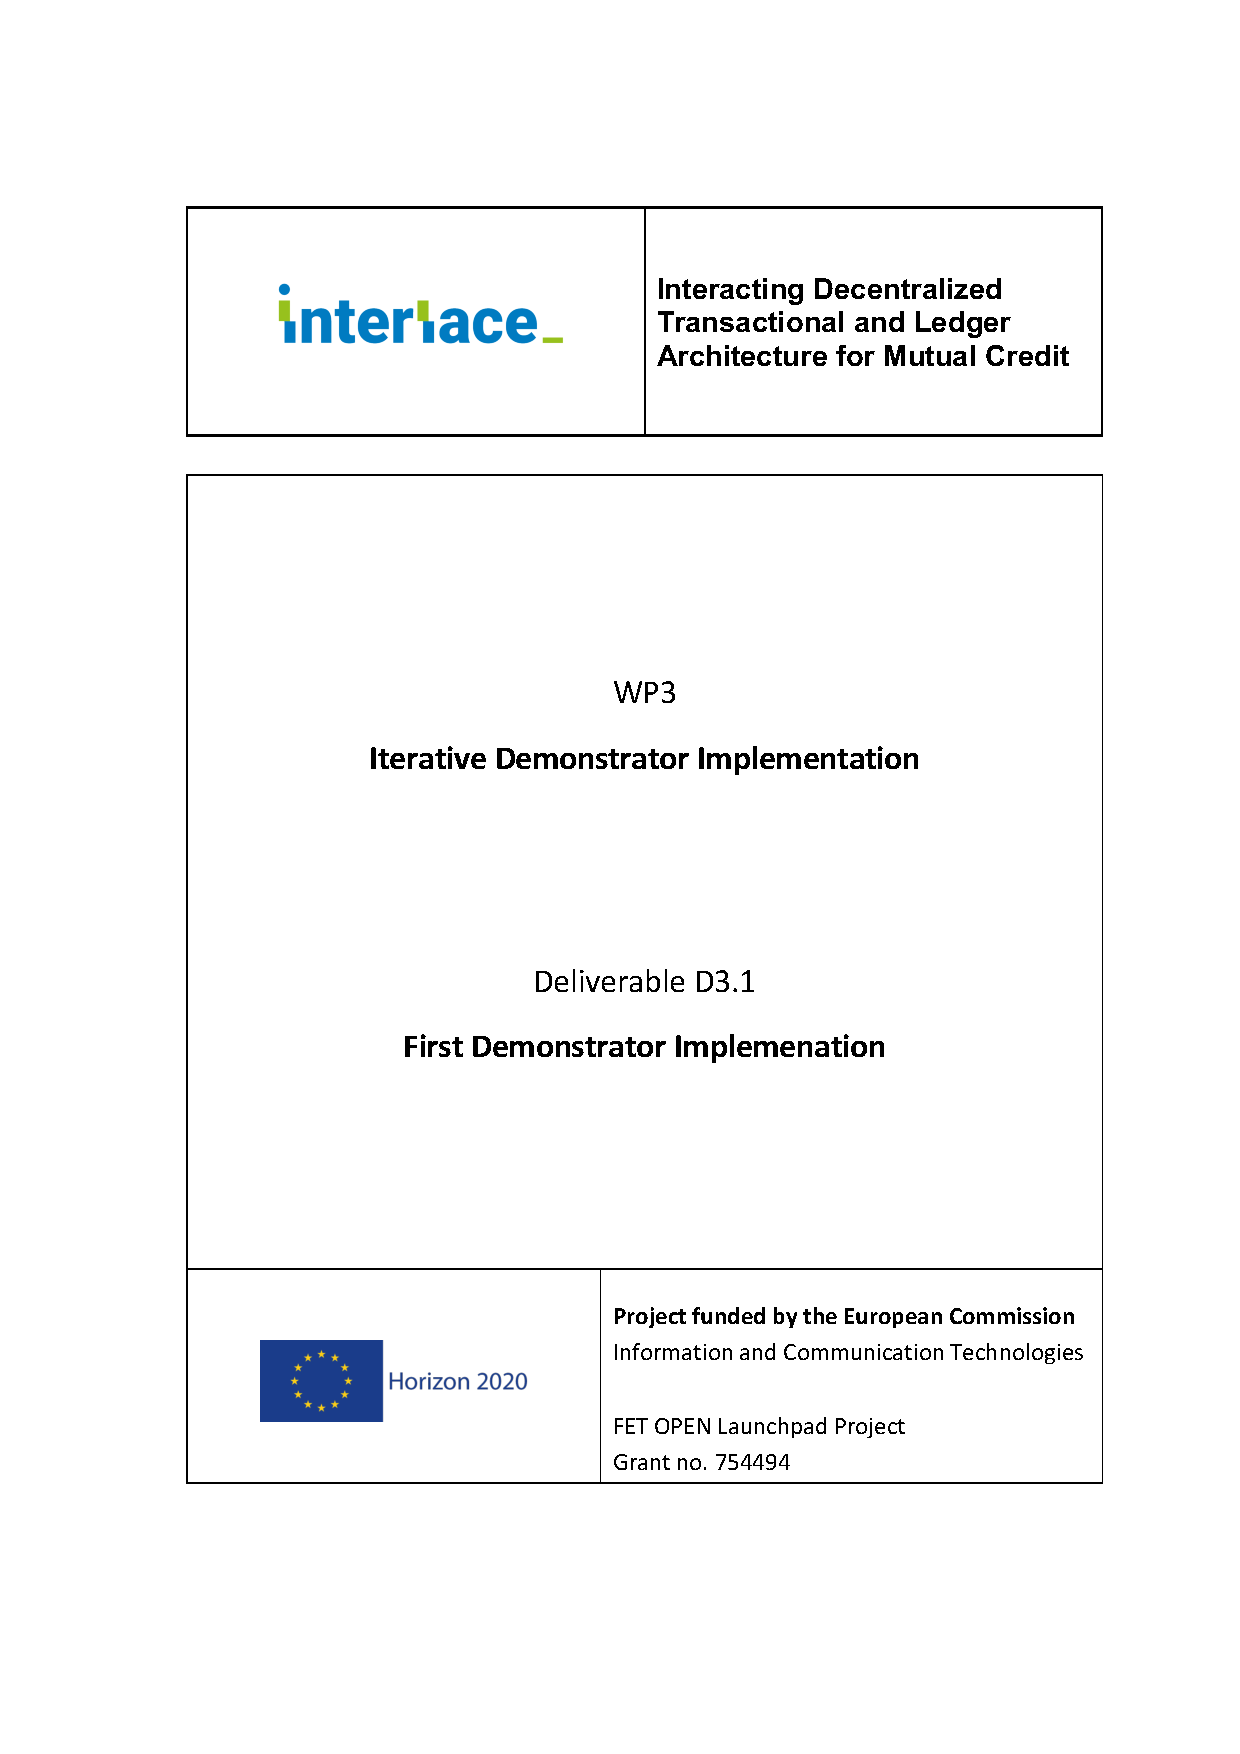
\includepdf[pages=-, scale=1.0]{Misc/Front}

%===================================================
%================== ABSTRACT
%===================================================
\thispagestyle{empty}

\begin{abstract}
\normalsize
This report describes the ASIM implementation defined by Deliverable D2.1: Requirements and Architecture Definition as well as mechanisms used to ensure a stable and shared runtime environment in order to guarantee testability and easy execution of the ASIM-model reflecting
the business logic. Further, the code structure is described and examined in terms of necessary deviations based on the original ASIM definitions in D2.1. Finally a presentation of the enclosed runtime environment is given and elaborated about the future connection to the actual blockchain-driven backend.
\end{abstract}

\newpage

%===================================================
%================== TABLE OF CONTENTS
%===================================================
\tableofcontents

%===================================================
%================== CHAPTERS
%===================================================
\chapter{Introduction}
\label{ch:Introduction}

\vspace{-1cm}
\begin{center}
Eduard Hirsch and Paolo Dini
\end{center}


...

bla bla

...














\newpage












\chapter{Refinement of the INTERLACE Business Logic Specification}
\label{ch:UpdateBLS}

\vspace{-1cm}
\begin{center}
Paolo Dini, Luca Carboni, Giuseppe Littera, Egon B\"orger and Chrystopher Nehaniv
\end{center}

\section{Context and Overview}
The business logic specification provided in Deliverable D2.1 \cite{INTERLACE_D21} concerns user-initiated transactions. Although this is a subset of all possible operations (initiated by the users or by the System, which we refer to as $SysAdmin$) that a mutual credit system platform must support, it is a viable starting point for testing an initial executable CoreASIM model. D2.1 did not provide all the details of the transaction request operations, it left their specification at a fairly abstract level. This chapter provides the next step in the iterative refinement of the specification in the form of a detailed description of the Permissioning workflow, whose implementation as part of the CoreASIM model is then described in Chapter \ref{ch:CoreAsimImplementation}. The description of the Permissioning iterative refinement relies on graphical and tabular depictions of the variables and functions involved. As this reflects the process that was used to build a shared understanding within the INTERLACE team itself, it is hoped that it will also make it easier for newcomers to the INTERLACE open source community to understand the implementation and the logic behind it.

At the highest level the INTERLACE transactional platform is a dynamic information system that interacts with a database at the backend and with live users at the front-end. As already discussed in D2.1, the transaction engine relies on many categories of concepts that, together, constitute the domain model of the system. According to the ASM methodology \cite{BoergerStaerk2003}, these have been subdivided into ASIMs comprised of rules, programs, and various kinds of functions. Whereas concepts such as `user' or 'transaction amount' are immediately clear, many more concepts and data structures are needed to specify and model the system. Before we get into the details, it helps to introduce three high-level perspectives through which the transaction engine can be characterized as an abstract machine and as a social construct: privacy (private-public dichotomy), dynamics (frequency domain), and transaction workflow already mentioned (time domain).

\begin{figure}[h]
\vspace{-0.5cm}
\centering
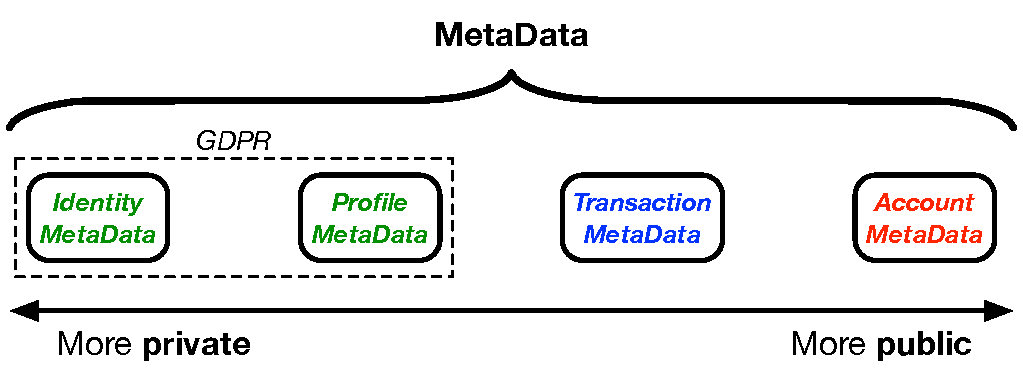
\includegraphics[width=12cm]{Figures/Private_Public_MetaData}
\caption{\small\textbf{Relative privacy of different types of meta-data of the INTERLACE transaction engine}}
\label{fig:privatepublicmetaData}
\vspace{-0.5cm}
\end{figure}

The first principle that influences the architecture of the system at a global level is the need to comply with the GDPR directive. Figure \ref{fig:privatepublicmetaData} shows how from this point of view the Transaction MetaData can be regarded as more public than the Account MetaData since it only contains a memo describing the transaction. The figure also shows that sub-dividing the meta-data in this manner makes it possible to limit the need for GDPR compliance\footnote{General Data Protection Regulation: \url{https://www.eugdpr.org/}} only to the Identity and Profile MetaData. Second, in a physics context the level of dynamicity of the variables could be described as the characteristic frequency (or its inverse, time-scale) at which different kinds of variables change as the transactional workflow is carried out. Figure \ref{fig:staticdynamicmetadata} shows how this principle applies to the system's meta-data.

\begin{figure}[h]
\vspace{-0.5cm}
\centering
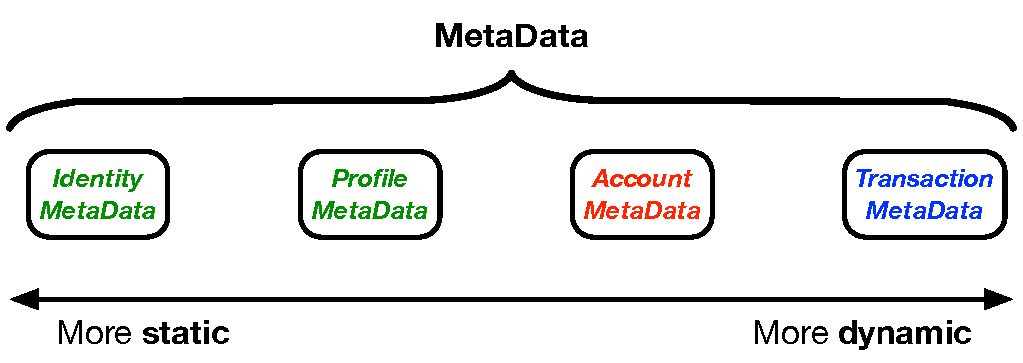
\includegraphics[width=12cm]{Figures/Static_Dynamic_MetaData}
\caption{\small\textbf{Relative dynamicity of different types of meta-data of the INTERLACE transaction engine}}
\label{fig:staticdynamicmetadata}
\vspace{-0.5cm}
\end{figure}

Third, Figure \ref{fig:transactabilitywkflow} shows the high-level view of the transaction workflow, including how the PreviewRequest and PerformRequest rules specified in D2.1 map onto it. The process starts on the left of the figure, when a user or $SysAdmin$ initiates the request for a transaction. The request must pass the three tests shown: Transfer Types, Account Connectivity and, in Inter-Circuit operations, the euroFee is calculated and shown to the user. At this point the user is shown a preview screen that summarizes all the transaction data. When the user issues the command to proceed, the first two tests are repeated and a final test on the account limits (e.g.\ sufficient funds) is performed. If also this fourth test is passed, the transaction is executed.

\begin{figure}[h]
\centering
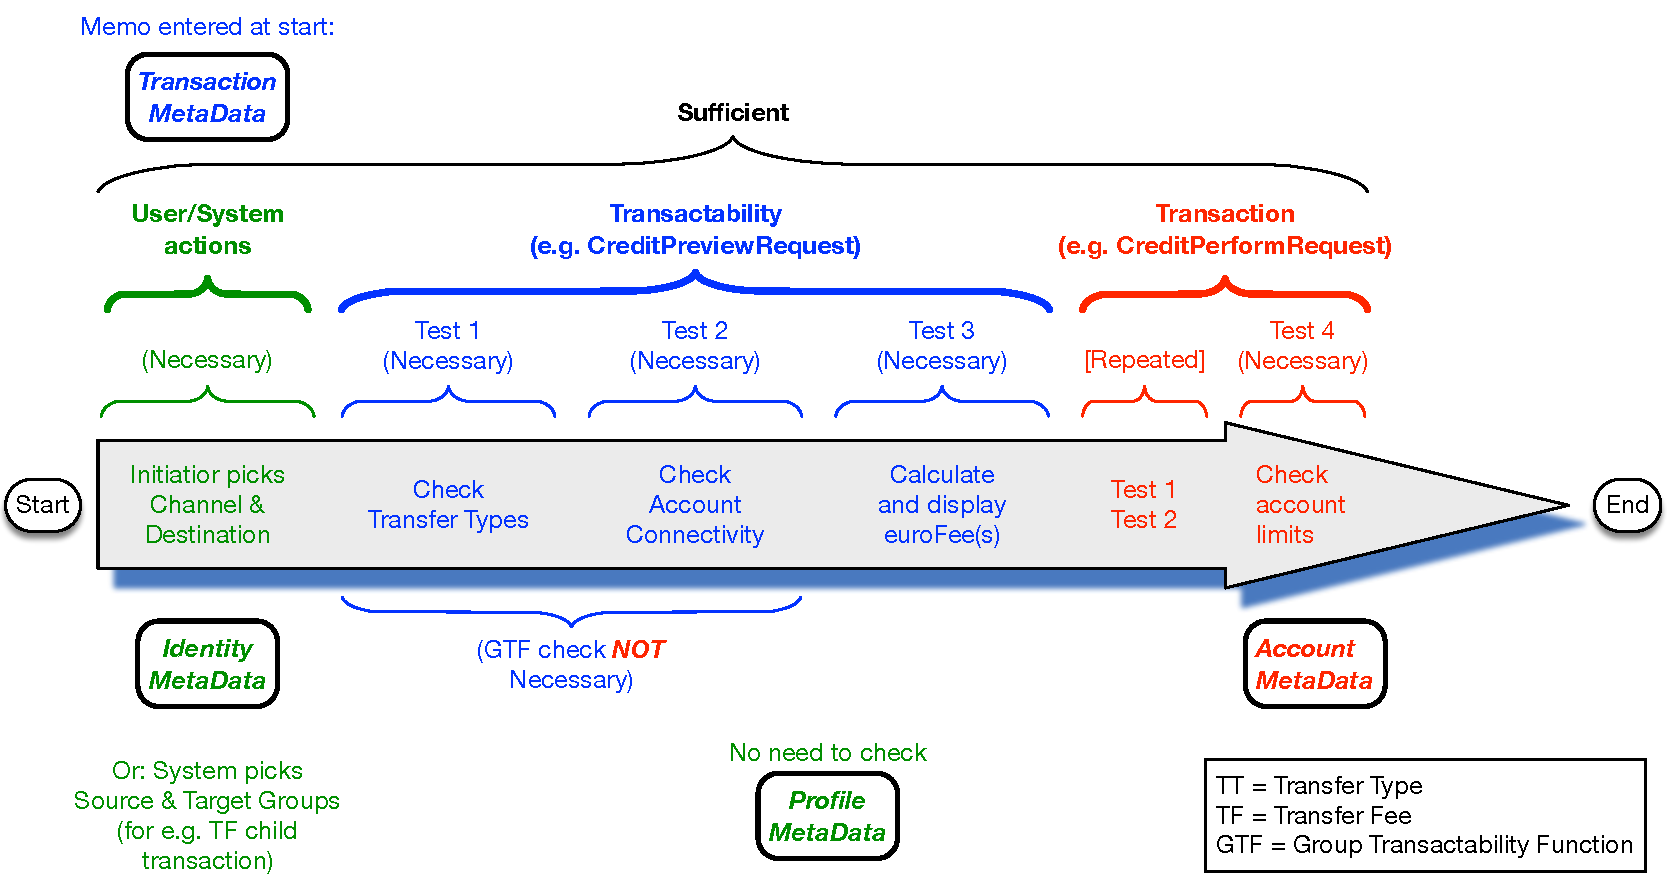
\includegraphics[width=17.5cm]{Figures/Transactability_Workflow}
\caption{\small\textbf{High-level workflow of the Permissioning process for user- or system-initiated transactions}}
\label{fig:transactabilitywkflow}
\end{figure}

In the following, first we provide a taxonomy of all the terms and concepts used and needed by the model, and then proceed to explain each step of the transaction workflow.


\section{Permissioning Model Taxonomy}
\subsection{Users and Groups}
Users are organized by user types called `Groups'. Consistently with the Appendix, in mathematical notation a $Group$ is a set of $group$s, such that $group \in Group$. However, also an individual $group$ is a set, specifically it is a set of users of the same type. Therefore, the group $Retail$ is capitalized, whereas a single shop is a $retail$. In the original Sardex platform not much distinction is made between users and groups. However, in the current INTERLACE specification we do need to discriminate between them.

\begin{quote}
\vspace{-0.3cm}
\small
For example, when describing a Debit transaction use case, at the User level the Seller initiates the Debit transaction to draw funds from the Buyer's account. In this scenario, therefore, the Seller is the $fromUser$ and the Buyer is the $toUser$. However, at the Group level things are different. As part of the transactability tests to be described fully in later sections, to each group that initiates a transaction ($fromGroup$) is associated a set of groups that can be on the receiving end of that transaction. In the case of a Debit transaction, whereas the \emph{request} goes to the Buyer, the receiving end of the transaction is not the Buyer, it is the Seller. Therefore, in a Debit operation $fromGroup$ = Seller, and $toGroup$ = Seller too!
\vspace{-0.3cm}
\end{quote}

The possible confusion created by debit transactions is resolved at the level of the accounts. See Section \ref{sec:intlevels}. The original Sardex system divided its users into 29 different groups. This generated a great deal of complexity that is drastically reduced in the INTERLACE version of the platform. The new user type taxonomy involves only 9 groups, as shown in Table \ref{tab:groups}.

%\setcounter{table}{0}
\setlength{\tabcolsep}{10pt}
\begin{table}[h]
\vspace{-0.3cm}
\begin{centering}
\small
{
\begin{tabular}{ r | l  }
\hline
\textbf{Group}	& \textbf{Description of Element of Group} \\
\Xhline{1.5pt}
$Welcome$ & User who has joined and signed the contract, but has not yet been cleared to start trading \\
\hline
$Retail$ & Retailer who can \emph{only} participate in B2C operations (not B2E and not B2B) \\
\hline
$Company$ & Company, which could be a retailer, that can use B2E and B2B but \emph{not} B2C \\
\hline
$Full$ & This group has all the functions of $Retail$ and of $Company$ \\
\hline
$Employee$ & Employee of a $company\in Company$ or of a $full \in Full$ \\
\hline
$On$\_$Hold$ & User whose privileges have been suspended (for whatever reason) \\
\hline
$Consumer$ & Person not registered to the circuit who can only interact through B2C Use Case 2 \\
\hline
$Consumer$\_$Verified$ & $consumer$ who has registered and can now also purchase with SRD (B2C Use Case 3)  \\
\hline
$MNGR$ & Manager of the circuit (e.g.\ Sardex S.p.A.) acting as a $company$ rather than $SysAdmin$ \\
\Xhline{1.5pt}
\end{tabular}
}
\caption{\small\textbf{New user types (groups) for the INTERLACE platform}}
\label{tab:groups}
\end{centering}
\vspace{-0.7cm}
\end{table}

$SysAdmin$ is not defined explicitly as a group, in this model, although technically it too is a user type. $SysAdmin$ has special privileges, some of which are discussed where relevant in what follows. We do not use lower-case for $MNGR$ and $SysAdmin$ because there is only one of each.

\subsection{Currencies and Channels}
As shown in Figure \ref{fig:currchan}, the Sardex/INTERLACE platform supports transactions in both Sardex credits (SRD) and Euros (EUR) over two kinds of channels. `Service' refers to transactions mediated either by a computer (web application) or a mobile phone (either a web application or a phone App). `POS' means `Point of Sale' and refers to the standard terminal used by retailers that accepts credit or debit cards, through which SRD transactions can be routed via an API. The figure also shows the four possible $\{ currency, channel \}$ combinations that we need to support in the definition and implementation of the permissioning tests discussed in the next sections.

\begin{figure}[h]
\vspace{-0.3cm}
\centering
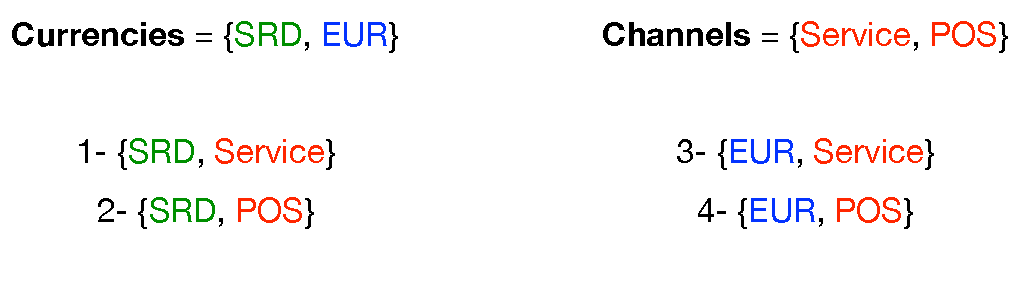
\includegraphics[width=10cm]{Figures/Curr_Chan}
\caption{\small\textbf{Currencies and channels supported by the platform}}
\label{fig:currchan}
\vspace{-0.5cm}
\end{figure}

\subsection{Accounts}
As shown in Table \ref{tab:accounts}, the accounts implemented in the model reflect the current operations of the Sardex system and the needs of a wide range of business operations and interactions. Some of the account types, for example MIRROR, may be phased out as the high-level architecture of the family of Sardex circuits grows and different algorithms replace the current strict controls on the balance of payments between different circuits. Also an account can be referred to as $fromAcct$ or $toAcct$ depending on its role in the transaction. See Section \ref{sec:intlevels}.

\setlength{\tabcolsep}{10pt}
\begin{table}[htbp]
\vspace{-0.3cm}
\begin{centering}
\small
{
\begin{tabular}{ r | l  }
\hline
\textbf{Account}	& \textbf{Description} \\
\Xhline{1.5pt}
$CC$ & Standard Sardex credits (SRD) account \\
\hline
$DOMU$ & SRD account used for larger operations, such as for real estate or capital equipment\\
\hline
$MIRROR$ & Account controlled by $MNGR$, used for inter-circuit purchases \\
\hline
$Income$ & Statistical EUR account owned by $retail$ or $full$ that collects B2C payments\\
\hline
$Prepaid$ & Statistical EUR account from which the 2\% child B2C transaction fee is drawn \\
\hline
$Bisoo$ & Statistical EUR account used by $consumer$ to pay into Income \\
\hline
$Topup$ & Statistical EUR account used by $MNGR$ to recharge $retail$'s Prepaid account upon receipt of \\
&\hspace{0.5cm} EUR payment. It is recharged back to zero gradually with each B2C transaction. \\
\Xhline{1.5pt}
\end{tabular}
}
\caption{\small\textbf{New user types (groups) for the INTERLACE platform}}
\label{tab:accounts}
\end{centering}
\vspace{-0.3cm}
\end{table}

\subsection{Account Limits}
Table \ref{tab:accountLimits} shows the account limit parameters that apply to the SRD accounts CC, DOMU, and MIRROR. The credit limit is straightforward, it is the maximum negative value the account balance can reach. However, note that it is expressed as a \emph{positive} number. This is important to keep in mind for the calculations that are based on the value of this parameter. The credit limit is set at the time a user signs the contract with Sardex and is reviewed at least every year after that. The upper limit is, similarly, the maximum value the balance of the account is allowed to reach. Whereas the credit limit can be considered to be a safety measure for the circuit, the upper limit is more a safety measure for the user, since if the balance becomes too large-positive it may be difficult for the user to find ways to spend the credits in a useful time (for the user). Capacity is the maximum total sale volume that the user commits to accepting in one year. The alerts are safety buffers set by the user to alert him/her when the account balance and/or the sale volume approach these limits.

\setlength{\tabcolsep}{10pt}
\begin{table}[htbp]
\vspace{-0.3cm}
\begin{centering}
\small
{
\begin{tabular}{ r | l  }
\hline
\textbf{Account Limit Parameter} & \textbf{Description} \\
\Xhline{1.5pt}
$creditLimit$& Maximum negative SRD balance allowed (\emph{positive} number) \\
\hline
$upperLimit$ & Maximum positive SRD balance allowed (positive number)\\
\hline
$capacity$ & Maximum {\bf sale} volume allowed in one year \\
\hline
$lowBalanceAlert$ & Buffer set by user: alert if $(creditLimit + balance) < lowBalanceAlert$\\
\hline
$highBalanceAlert$ & Buffer set by user: alert if $(upperLimit - balance) < highBalanceAlert$ \\
\hline
$highVolumeAlert$ & Buffer set by user: alert if $(capacity - saleVolume) < highVolumeAlert$ \\
\Xhline{1.5pt}
\end{tabular}
}
\caption{\small\textbf{Account limit parameters}}
\label{tab:accountLimits}
\vspace{-0.3cm}
\end{centering}
\end{table}

Figure \ref{fig:accountLimitsCC} shows a visualization of the account limits that apply to SRD accounts such as $CC$. The thick vertical green arrows highlight that the calculation of the sale volume is defined as \emph{the sum of all the sales performed in one year}. In this example, the sum of all the vertical green arrows is 50,000. Figure \ref{fig:accountLimitsPrepaid} is a visualization of the $Prepaid$ EUR account, which is recharged or topped up once in a while (\euro 400 in the figure) and slowly drawn down by B2C transaction fees (see B2C Use Case 2 in Figure \ref{fig:B2C1} below).

\subsection{Operations}
As already specified in D2.1, transactions are effected through two operations: $credit$ and $debit$:
\begin{align}
Operation = \{ credit, debit \}.
\end{align}

\begin{figure}[h]
\vspace{-0.5cm}
\centering
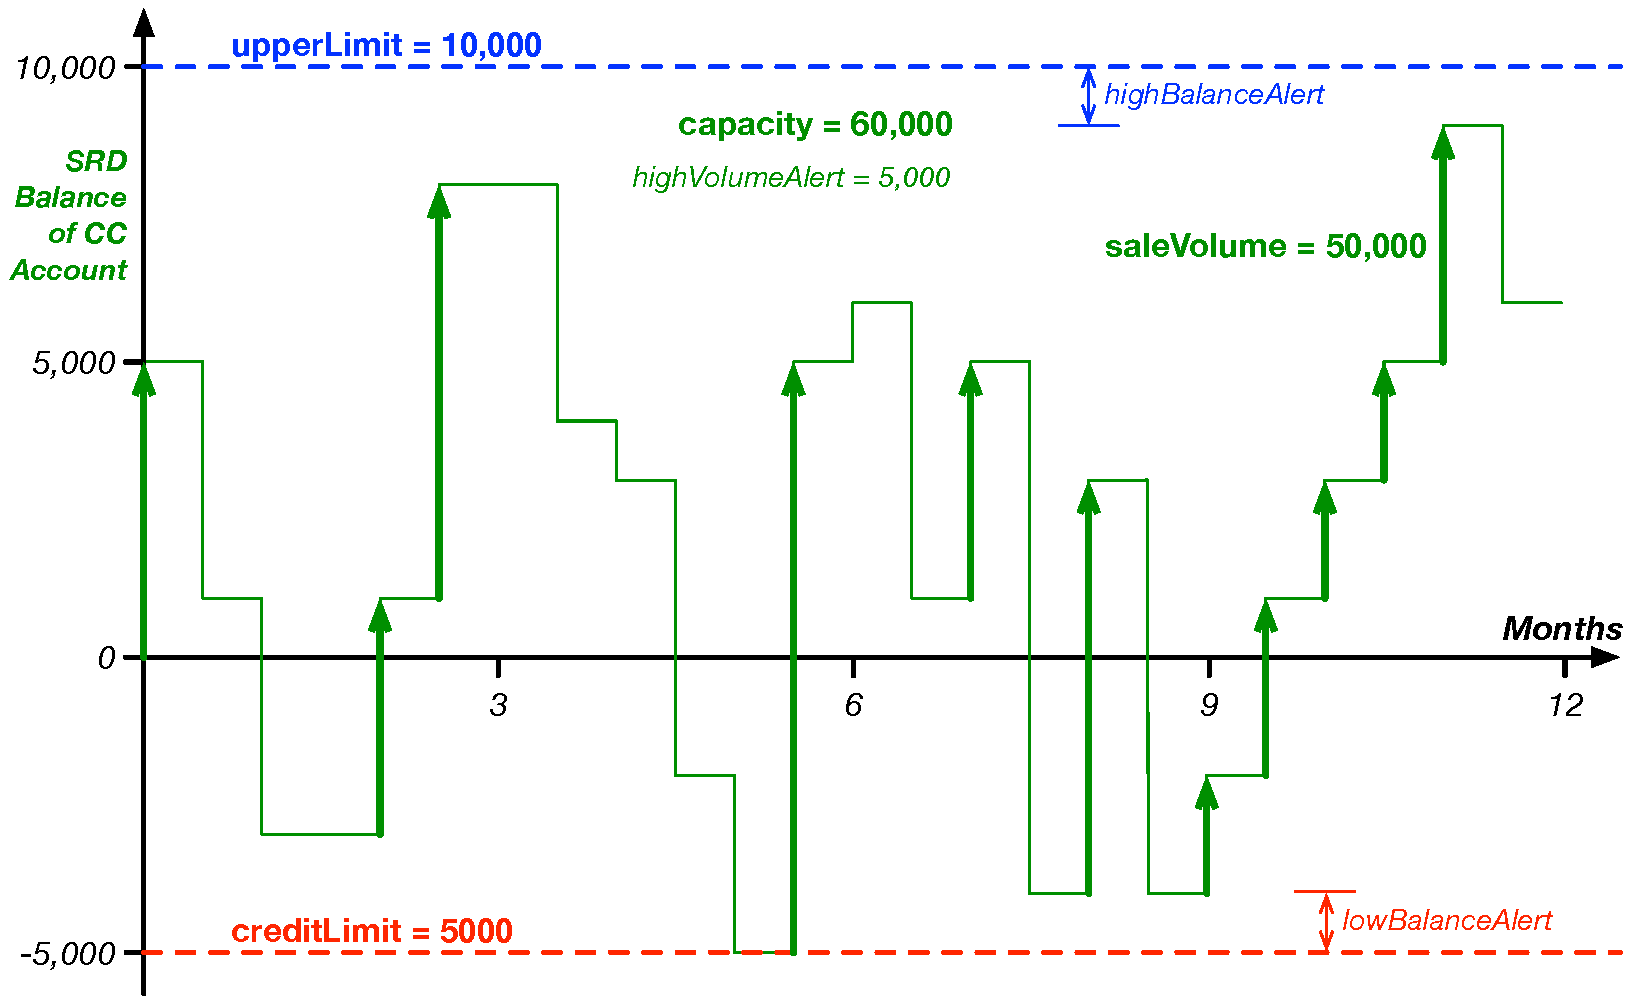
\includegraphics[width=15cm]{Figures/Account_Limits_CC}
\caption{\small\textbf{Visualization of the $CC$ account limits}}
\label{fig:accountLimitsCC}
\vspace{-0.8cm}
\end{figure}


\begin{figure}[htbp]
\vspace{-0.8cm}
\centering
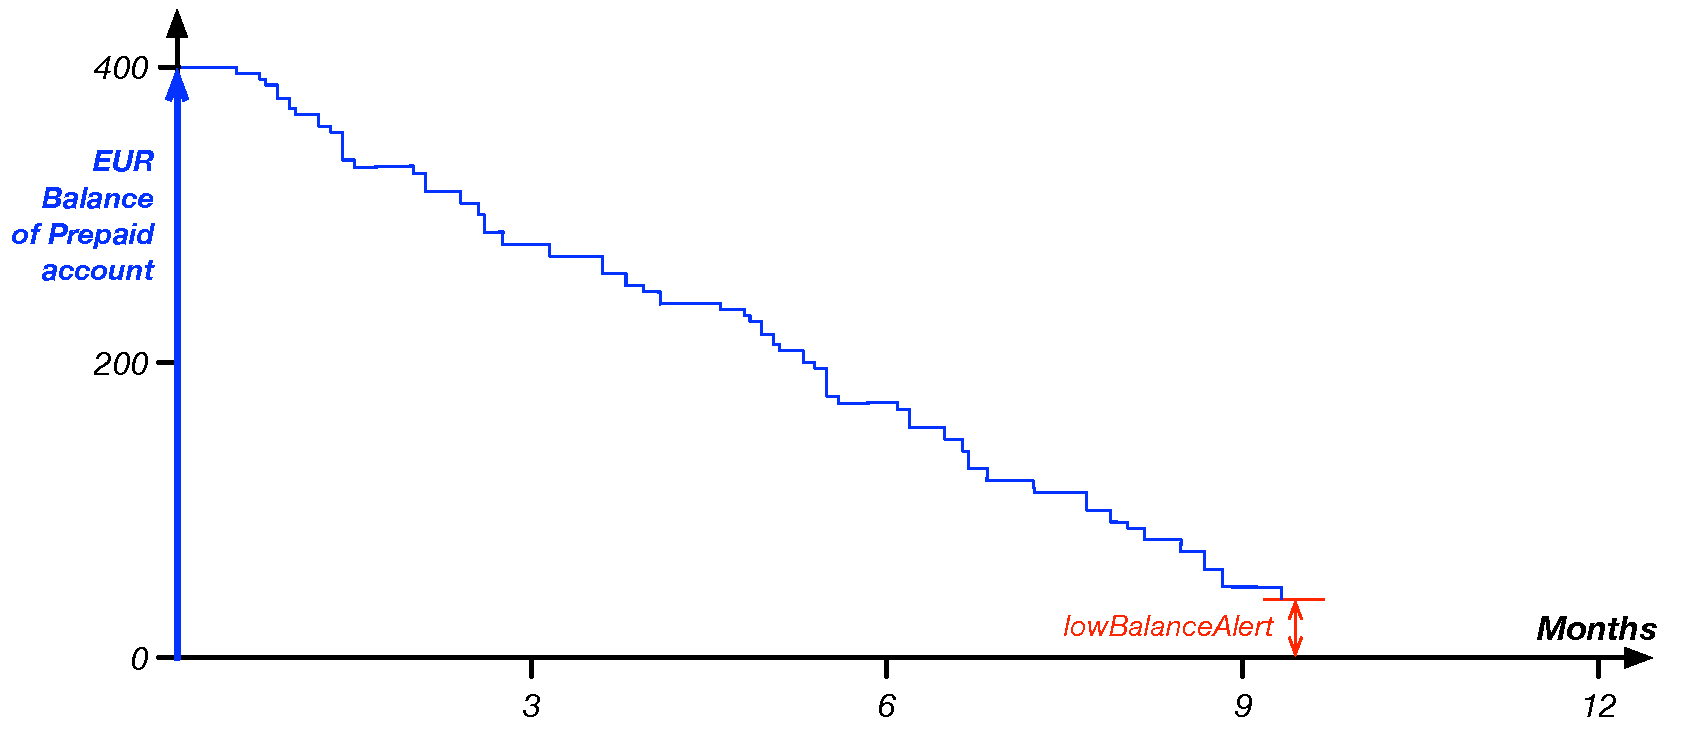
\includegraphics[width=15.6cm]{Figures/Account_Limits_Prepaid}
\caption{\small\textbf{Visualization of the $Prepaid$ account limit}}
\label{fig:accountLimitsPrepaid}
\vspace{-0.5cm}
\end{figure}


\subsection{Interaction Levels}
\label{sec:intlevels}
The interactions between circuit participants can be described from different points of view that correlate loosely to a stack view of the system. As shown in Figure \ref{fig:stack}, it is helpful to identify qualitatively the different levels of such a stack, acknowledging that it is \emph{more} than a networking communication stack in terms of scope but \emph{less} than one in terms of precision. `A' and `B' refer to the Buyer and the Seller respectively. Figure \ref{fig:stack} extends the two communication levels described in D2.1, but does so qualitatively. For the purposes of the implementation, we need a smaller set of levels but a more precise and specific vocabulary to identify the end-points of the transaction.

\begin{figure}[H]
\centering
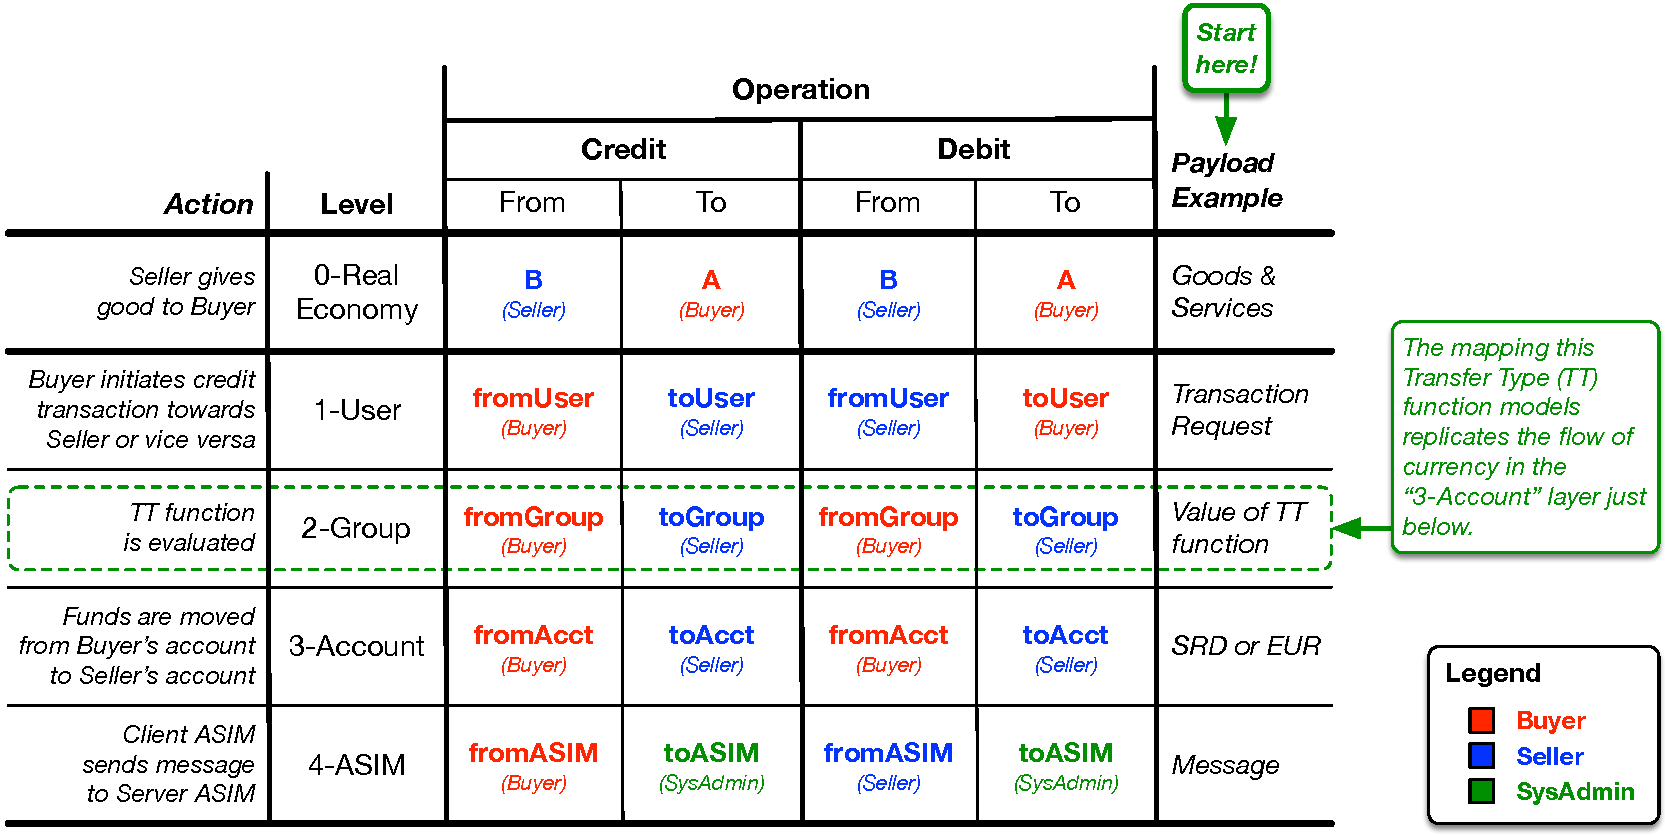
\includegraphics[width=17.5cm]{Figures/Stack}
\caption{\small\textbf{Stack view of the INTERLACE communication, economic, and financial  interactions}\\
(Stack view of from where to where the different payloads are moved in interactions)}
\label{fig:stack}
\vspace{-0.5cm}
\end{figure}

Figure \ref{fig:vocabulary} shows this additional information as concerns levels 1-4, which are labelled in the first column in the same way as in Figure \ref{fig:stack}, along with some more information. In particular, this figure could be seen to integrate aspects of Figures \ref{fig:stack} and \ref{fig:transactabilitywkflow}, with the purpose of facilitating the conceptual understanding of the specification. The different types of `MetaData' relevant to transactions are shown in the approximate position where they are polled. For example, the $\%$ of SRD accepted by a given user over 1000-EUR transaction values is part of the Profile MetaData of the $Company$ group but not the $Consumer$\_$Verified$ group's.

\begin{figure}[htbp]
\centering
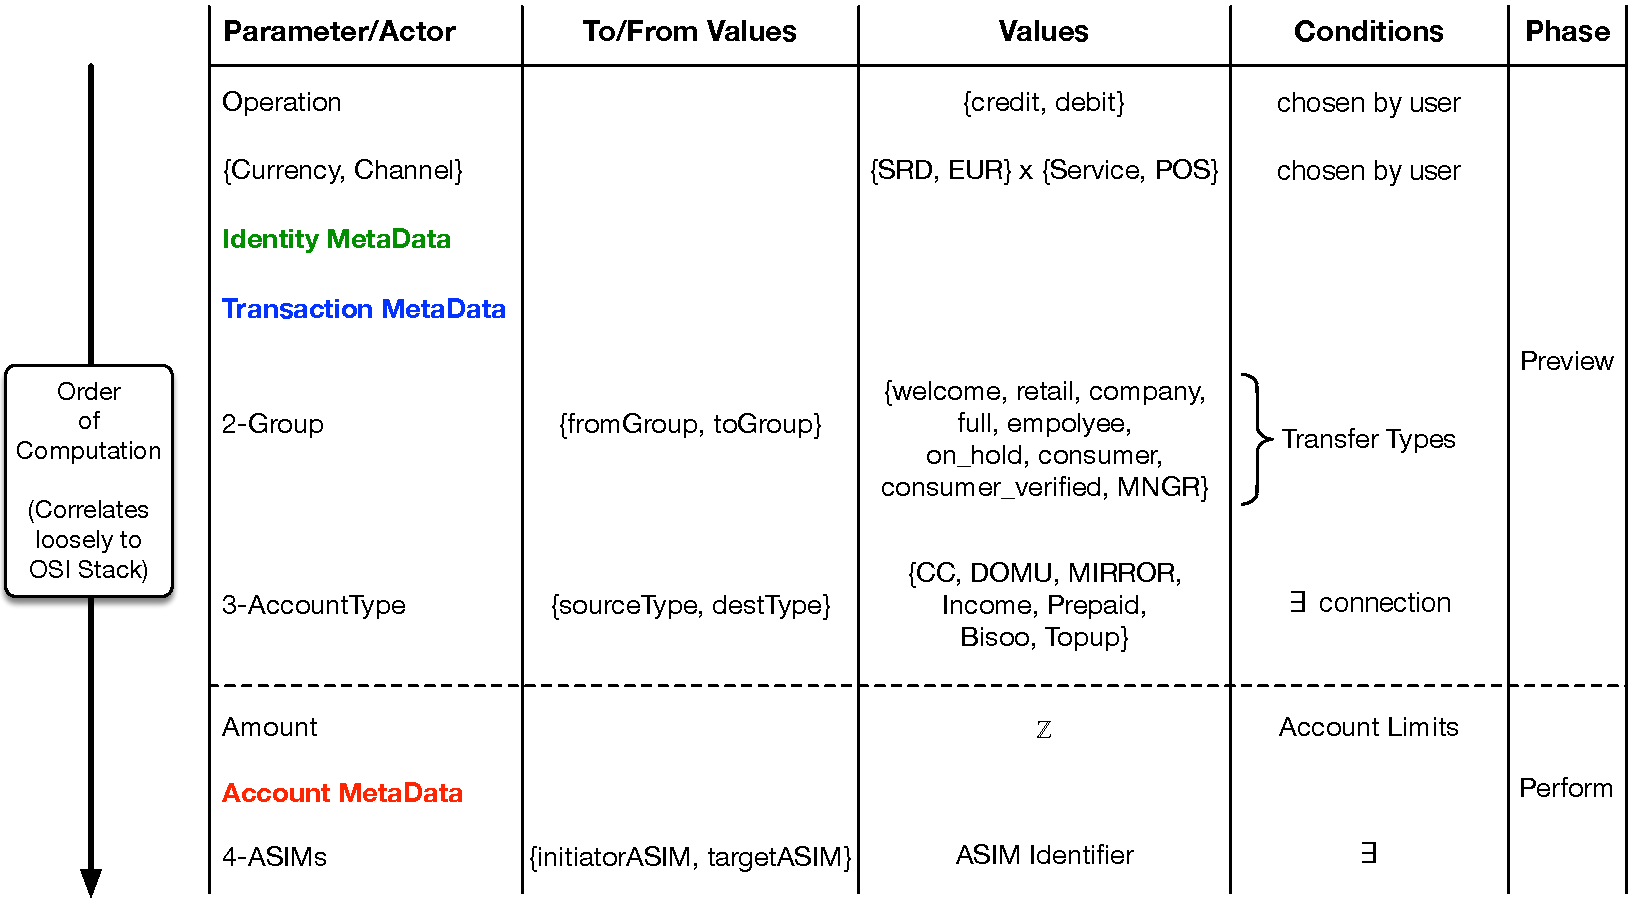
\includegraphics[width=17cm]{Figures/Vocabulary}
\caption{\small\textbf{Actors, parameters, levels, data structures, computational process, and conditions}}
\label{fig:vocabulary}
\end{figure}

\subsection{Visibility}
Figure \ref{fig:visibility} shows which groups ($toGroup$) are visible to which groups ($fromGroup$) by a `1' at the intersection of the $(row, column)$ corresponding to a choice of $(fromGroup, toGroup)$. For example, $Company$ is visible to $Employee$, meaning that $Employee$ can do a search for $Company$, but not vice versa. In this case $Employee$ is not visible due to privacy legislation.

\begin{figure}[H]
\centering
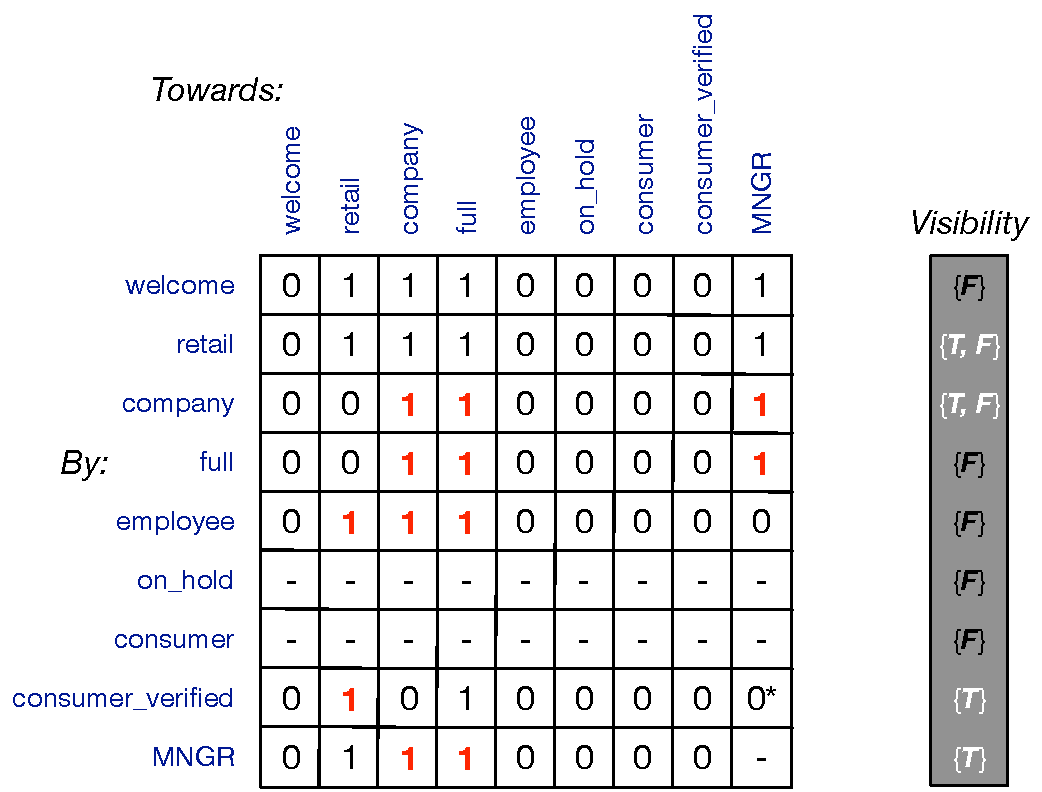
\includegraphics[width=12cm]{Figures/Visibility}
\caption{\small\textbf{Mutual visibility of different groups}}
\label{fig:visibility}
\vspace{-0.5cm}
\end{figure}

In general, transactability correlates to visibility. However, there is not a strict 1-1 relationship between them. For the example of a $company$ paying its own $employee$s as part of the B2E programme, $employee$ remains invisible to a search, but $company$ has the $username$ of the $employee$ and can perform a credit transaction to pay (part of) their salary.

On the right of Figure \ref{fig:visibility} we show that some groups are always invisible $\{ F \}$ others are always visibile $\{ T \}$, and others could be either $\{T, F\}$. For example, a company could be put in the shadow state if it has reached its maximum positive credit limit.

\subsection{B2C Operations}
This report extends the use cases covered by D2.1 by adding also the Business to Consumer (B2C) use cases. B2C was developed to increase the number and volume of transactions, i.e.\ the size of the Sardex economy, by extending the ability to transact in SRD to people not otherwise connected to the circuit. The principle involves offering the opportunity to $retail$ers to reward their EUR customers with an SRD rebate.

The amount of the reward is a percent, in SRD, of the amount in EUR paid by a $consumer$ to a $retail$, where the percent is set by $retail$ and it is an example of the $MetaData$ for this group. The reward is stored on a smart card that is offered to $consumer$ at the time of purchase. This is shown as a child transaction in B2C Use Case 2, Figure \ref{fig:B2C1}.

\begin{figure}[htbp]
\centering
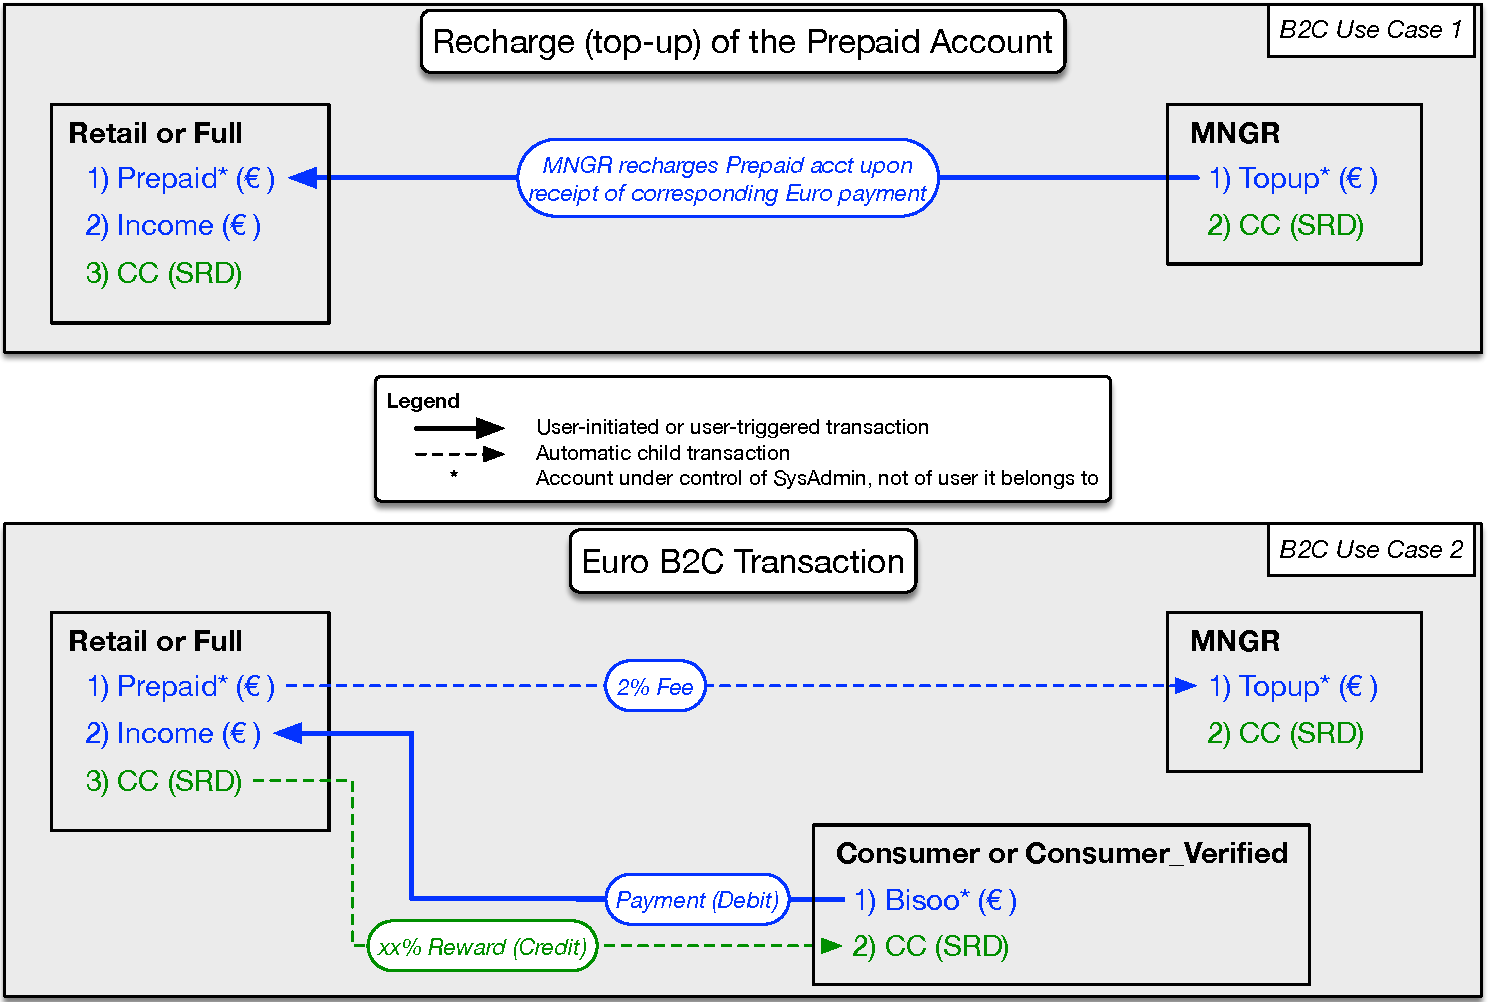
\includegraphics[width=15cm]{Figures/B2C1}
\caption{\small\textbf{Recharging of $retail$'s Prepaid account and standard B2C EUR transaction}}
\label{fig:B2C1}
\end{figure}

Use Case 2 also involves a second child transaction, a 2\% fee, in EUR, paid from $retail$'s Prepaid account to $MNGR$'s Topup account. The asterisks next to these account names, in the figure, indicate that these two accounts are \emph{owned} by these two users but are not \emph{controlled} by them. They are controlled by $SysAdmin$. These EUR accounts are `statistical' rather than `real', meaning that they simply keep track of actual EUR amounts but do not themselves hold Euros. Sardex S.p.A. would need to be a bank for that to be possible. For Use Case 2 to be executable, for a given $retail$er, its Prepaid account needs to have sufficient funds. When it runs out of statistical Euros, $retail$ can pay $MNGR$ some amount of Euros using any of the standard payment systems, through a bank or a payment service provider like PayPal. This triggers Use Case 1, also shown in Figure \ref{fig:B2C1}.

\begin{figure}[h]
\centering
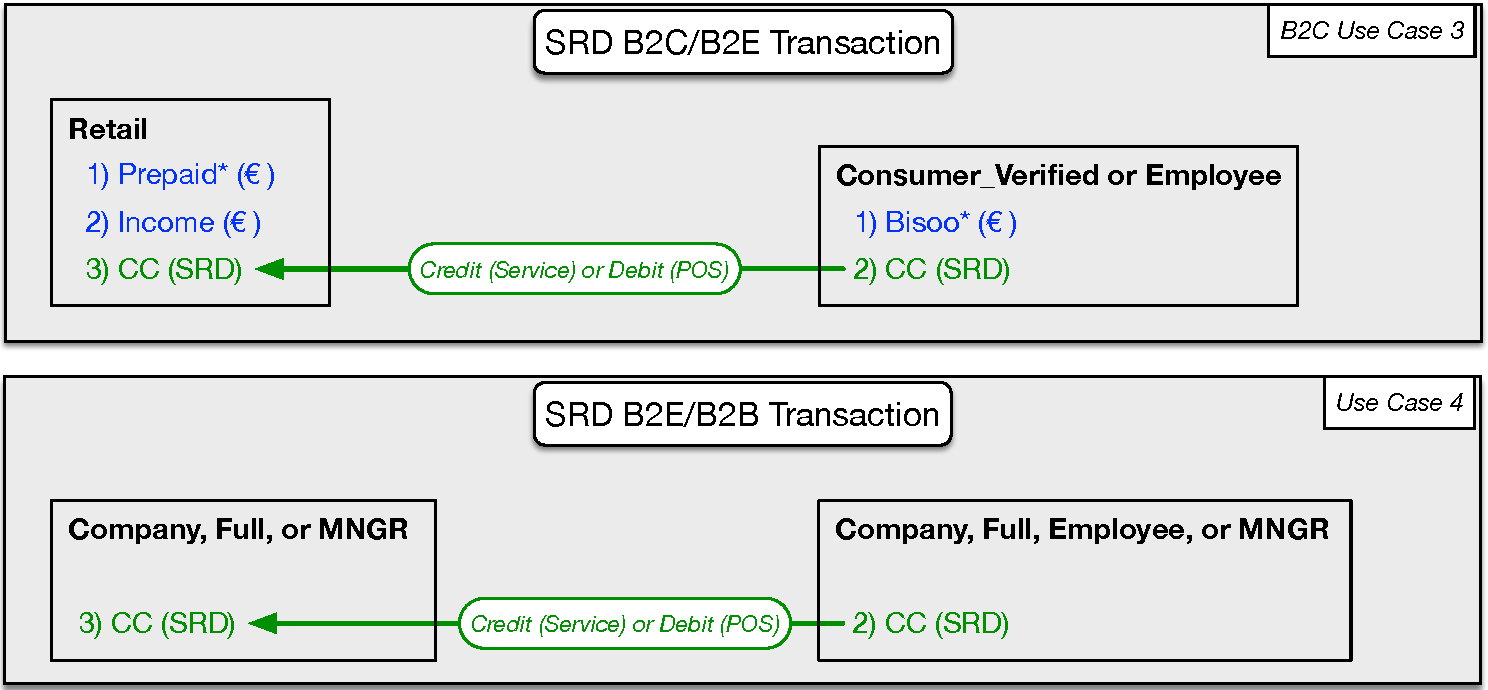
\includegraphics[width=15cm]{Figures/B2C2}
\caption{\small\textbf{SRD transactions for B2C, B2E, and B2B users}}
\label{fig:B2C2}
\end{figure}

Figure \ref{fig:B2C2} shows the SRD transaction a $consumer$ can perform, i.e.\ the spending of the SRD accumulated as rewards, once they have registered and have become $consumer$\_$verified$. The figure also shows that Use Case 3 is relevant also to $employee$s (B2E) and that Use Case 4 is relevant to both B2E users and to non-$retail$ company users (B2B).

\subsection{Initial Account State}
Table \ref{tab:InitialAccountSets} shows the initial allocation of accounts to the different user groups. The allocation is `initial' because  depending on the history of a given user the number of its accounts could change. For legal reasons, as a general principle \emph{change} can only mean \emph{increase}. In other words, once a user has become the owner of an account it can never be taken away from them, even if, for example, its access to it is suspended due to misbehaviour. Another example is a $Retail$ user who upgrades to the $Full$ group and a year later changes its mind and goes back to $Retail$. It will retain its DOMU account even if it won't be able to use it anymore.

{\bf Note: Each user can have no more than one account of a given type.}

\begin{table}[h]
\vspace{-0.5cm}
\begin{centering}
\small
{
\begin{tabular}{ r | l  }
\hline
\textbf{Group}	& {\bf Initial Account Set} \\
\Xhline{1.5pt}
$Welcome$	& $\{ \}$ \\
\hline
$Retail$		& $\{ CC, Prepaid^*, Income \}$ \\
\hline
$Company$	& $\{ CC, DOMU, Prepaid^* \}$ \\
\hline
$Full$		& $\{ CC, DOMU, Prepaid^*, Income \}$ \\
\hline
$Employee$	& $\{ CC \}$ \\
\hline
$On$\_$Hold$	& $\{  \}$ \\
\hline
$Consumer$	& $\{ CC, Bisoo^* \}$ \\
\hline
$Consumer$\_$Verified$ & $\{ CC, Bisoo^* \}$ \\
\hline
$MNGR$ 		& $\{ CC, Topup^*, MIRROR \}$ \\
\Xhline{1.5pt}
\end{tabular}
}
\caption{\small\textbf{Initial sets of accounts assigned to the groups}\\ (*Indicates an account under the control of $SysAdmin$, not of the user it belongs to.)}
\label{tab:InitialAccountSets}
\end{centering}
\vspace{-1cm}
\end{table}

The Prepaid account shown for $Company$ does not relate to B2C operations but to inter-circuit trade, which also involves a euroFee.

\section{Transactability Workflow}
\subsection{Identity MetaData}
Table \ref{tab:IdentityMetaData} collects the identity meta-data for all the groups. $MemberID$ is a unique identifier. $email$ and $phone$ are arrays to support multiple values of each. These values are set at registration and cannot be changed by the user.

The meta-data variables are not capitalized because they are assumed to be singletons: for a given member, e.g.\ a $company$, there is only one $memberID$. However, since there are many $memberID$s, one for each member, we could also say that $memberID \in MemberID$. Since there are cases where a user may have more than one meta-data variable, for example a company with more than one phone number, this is indicated in the Type column as an array, i.e.\ `String[ ]'.

\begin{table}[H]
\vspace{-0.5cm}
\begin{centering}
\small
{
\begin{tabular}{ r | c | l | l }
\hline
\textbf{Group}	& {\bf Identity MetaData} & {\bf Type} & {\bf Description} \\
\Xhline{1.5pt}
$Welcome$, $Retail$, $Company$,	& {\bf memberID}			&Integer	& Unique member identifier \\
$Full$, $Employee$, $On$\_$Hold$,	& {\bf email}				&String[]	& e-mail address \\		
$Consumer$\_$Verified$, $MNGR$	& {\bf phone}				&String[]	& phone number(s) \\
\hline
$Consumer$	& {\bf memberID}	&Integer & Unique member identifier \\
\Xhline{1.5pt}
\end{tabular}
}
\caption{\small\textbf{Identity MetaData for all the groups}}
\label{tab:IdentityMetaData}
\end{centering}
\vspace{-1cm}
\end{table}

\subsection{Profile MetaData}
Tables \ref{tab:ProfileMetaData1} and \ref{tab:ProfileMetaData2} show the profile meta-data, some of which the user can inspect and edit. For example, the user may wish to include his/her personal name in addition to the company name.

\setlength{\tabcolsep}{10pt}
\begin{table}[H]
\begin{centering}
\small
{
\begin{tabular}{ r | c | l | l }
\hline
\textbf{Group}	& {\bf Profile MetaData} & {\bf Type} & {\bf Description} \\
\Xhline{1.5pt}
			& \emph{(Obligatory MetaData)} & & \\
\cline{2-2}
$Welcome$	& {\bf entityName}$^*$		&String	& Legal entity name \\
			& {\bf entityAddress}$^*$		&String	& Legal entity's street address \\
			& {\bf gps}$^*$				&Double[]	& Legal entity's GPS coordinates \\			
			& {\bf VAT}$^*$				&String	& Legal entity's VAT number \\
			& {\bf capacity}				&Double	& Commitment to maximum yearly SRD volume \\
			& {\bf capacityDate}			&DateTime & Date capacity was set \\
\cline{2-2}
			 & \emph{(Optional MetaData)}& & \\
\cline{2-2}
			& {\bf firstName}$^*$			&String	& First name \\
			& {\bf surName}$^*$			&String	& Surname \\
\Xhline{1.5pt}
			& \emph{(Obligatory MetaData)} & & \\
\cline{2-2}
$Retail$		& {\bf entityName}$^*$		&String	& Legal entity name \\
			& {\bf entityAddress}$^*$		&String	& Legal entity's street address \\
			& {\bf gps}$^*$				&Double[]	& Legal entity's GPS coordinates \\			
			& {\bf capacity}				&Double	& Commitment to maximum yearly SRD volume \\
			& {\bf capacityDate}			&DateTime & Date capacity was set \\
			& {\bf rewardRate}$^{**}$		&Double	& \% reward rate to consumer, in SRD \\
			& {\bf euroFee}				&Double[]	& \% fee on B2C EUR sales, in EUR \\
			& {\bf acceptanceRate}$^{**}$	&Double	& Rate of SRD acceptance in consumer purchases\\
\cline{2-2}
			 & \emph{(Optional MetaData)}& & \\
\cline{2-2}
			& {\bf firstName	}$^*$			&String	& First name \\
			& {\bf surName}$^*$			&String	& Surname \\
\Xhline{1.5pt}
			& \emph{(Obligatory MetaData)} & & \\
\cline{2-2}
$Company$	& {\bf entityName}$^*$		&String	& Legal entity name \\
			& {\bf entityAddress}$^*$		&String	& Legal entity's street address \\
			& {\bf gps}$^*$				&Double[]	& Legal entity's GPS coordinates \\
			& {\bf VAT}$^*$				&String	& Legal entity's VAT number \\
			& {\bf capacity}				&Double	& Commitment to maximum yearly SRD volume \\
			& {\bf capacityDate}			&DateTime & Date capacity was set \\
			& {\bf creditPercent}			&Double	& \% SRD acceptance for transactions above 1000 \\
			& {\bf euroFee}				&Double[]	& \% fee on inter-circuit SRD sales, in EUR \\
\cline{2-2}
			 & \emph{(Optional MetaData)}& & \\
\cline{2-2}
			& {\bf firstName	}$^*$			&String & First name \\
			& {\bf surName}$^*$			&String & Surname \\
\Xhline{1.5pt}
			& \emph{(Obligatory MetaData)} & & \\
\cline{2-2}
$Full$		& {\bf entityName}$^*$		&String	& Legal entity name \\
			& {\bf entityAddress}$^*$		&String	& Legal entity's street address \\
			& {\bf gps}$^*$				&Double[]	& Legal entity's GPS coordinates \\
			& {\bf VAT}$^*$				&String	& Legal entity's VAT number \\
			& {\bf capacity}				&Double	& Commitment to maximum yearly SRD volume \\
			& {\bf capacityDate}			&DateTime & Date capacity was set \\
			& {\bf creditPercent}			&Double	& \% SRD acceptance for transactions above 1000 \\
			& {\bf rewardRate}$^{**}$		&Double	& \% reward rate to consumer, in SRD \\
			& {\bf euroFee}				&Double[]	& \% fees on B2C EUR sales, inter-circuit SRD sales, in EUR \\
			& {\bf acceptanceRate}$^{**}$	&Double	& Rate of credits acceptance in consumer purchases\\
\cline{2-2}
			 & \emph{(Optional MetaData)}& & \\
\cline{2-2}
			& {\bf firstName}$^*$			&String	& First name \\
			& {\bf surName}$^*$			&String	& Surname \\
\Xhline{1.5pt}
			& \emph{(Obligatory MetaData)} & & \\
\cline{2-2}
$Employee$	& {\bf firstName}$^*$			&String	& First name \\
			& {\bf surName}$^*$			&String	& Surname \\
			& {\bf employedBy}			&String	& Name of legal entity employed by \\
\Xhline{1.5pt}
\end{tabular}
}
\caption{\small\textbf{Profile MetaData for the $Welcome$, $Retail$, $Company$, $Full$, and $Employee$ groups}\\
($^*$Indicates fields that can be modified by the user)\\
($^{**}$Indicates fields that can be modified by the user but that are updated only at a fixed time interval)}
\label{tab:ProfileMetaData1}
\end{centering}
\end{table}


\setlength{\tabcolsep}{5pt}
\begin{table}[H]
\begin{centering}
\small
{
\begin{tabular}{ r | c | l | l }
\hline
\textbf{Group}	& {\bf Profile MetaData} & {\bf Type} & {\bf Description} \\
\Xhline{1.5pt}
			& \emph{(Obligatory MetaData)} & & \\
\cline{2-2}
$On$\_$Hold$	& {\bf entityName}$^*$		&String	& Legal entity name \\
			& {\bf entityAddress}$^*$		&String	& Legal entity's street address \\
			& {\bf gps}$^*$				&Double[]	& Legal entity's GPS coordinates \\
			& {\bf VAT}$^*$				&String	& Legal entity's VAT number \\
			& {\bf capacity}				&Double	& Commitment to maximum yearly SRD volume \\
			& {\bf capacityDate}			&DateTime & Date capacity was set \\
			& {\bf creditPercent}			&Double	& \% SRD acceptance for transactions above 1000 \\
			& {\bf rewardRate}$^{**}$		&Double	& \% reward rate to consumer, in SRD \\
			& {\bf euroFee}				&Double[]	& \% fees on B2C EUR sales, inter-circuit SRD sales, in EUR \\			& {\bf acceptanceRate}$^{**}$	&Double	& Rate of credits acceptance in consumer purchases\\
\cline{2-2}
			 & \emph{(Optional MetaData)}& & \\
\cline{2-2}
			& {\bf firstName}$^*$			&String	& First name \\
			& {\bf surName}$^*$			&String	& Surname \\
\Xhline{1.5pt}
$Consumer$	& 	& &  \\
\Xhline{1.5pt}
			& \emph{(Obligatory MetaData)} & & \\
\cline{2-2}
$Consumer$\_$Verified$ & {\bf firstName}$^*$	&String	& First name \\
			& {\bf surName}$^*$			&String	& Surname \\
\Xhline{1.5pt}
			& \emph{(Obligatory MetaData)} & & \\
\cline{2-2}
$MNGR$ 		& {\bf entityName}$^*$		&String	& Legal entity name \\
			& {\bf entityAddress}$^*$		&String	& Legal entity's street address \\
			& {\bf gps}$^*$				&Double[]	& Legal entity's GPS coordinates \\
			& {\bf VAT}$^*$				&String	& Legal entity's VAT number \\
			& {\bf capacity}				&Double	& Commitment to maximum yearly SRD volume \\
			& {\bf capacityDate}			&DateTime & Date capacity was set \\
			& {\bf creditPercent}			&Double	& \% SRD acceptance for transactions above 1000 \\
\Xhline{1.5pt}
\end{tabular}
}
\caption{\small\textbf{Profile MetaData for the $On$\_$Hold$, $Consumer$, $Consumer$\_$Verified$, and $MNGR$ groups}\\
($^*$Indicates fields that can be modified by the user)\\
($^{**}$Indicates fields that can be modified by the user but that are updated only at a fixed time interval)
}
\label{tab:ProfileMetaData2}
\end{centering}
\vspace{-1.5cm}
\end{table}

\subsection{Transfer Types}
As shown in Figure \ref{fig:transactabilitywkflow}, the first test for transactability involves so-called Transfer Types. Transfer Types are mathematical functions of the {\bf source} groups ($fromGroup$s) whose values are sets of {\bf destination} groups ($toGroup$s). There is one different function for each combination of ordered pairs $(x, y)$, where $x \in \{ credit, debit \}$ and $y \in \{ SRD, EUR \}$, leading to four different functions. However, it is simpler and also easier to implement to express them as a single function of 3 parameters. Formally,
\begin{align}
TT\colon &Operation \times Currency \times Group\ \rightarrow\ Powerset(Group),
\end{align}
where
\begin{align}
Group &= \{ Welcome, Retail, Company, Full, Employee, On\text{\_}Hold,  \nonumber \\
		& \qquad\qquad\qquad\qquad\qquad\qquad\qquad
			Consumer, Consumer\text{\_}Verified, MNGR \}.
\end{align}
With an abuse of notation and overloading the terminology we define for convenience the following sets of target groups ($toGroups$) as different ``transfer types'':
\begin{align*}
TT_1 &= \{ Retail \},		&& TT_2 = \{ Retail, Company \},	&& TT_3 = \{ Company, Employee \} \\
TT_4 &= \{ Company \},	&& TT_5 = \{ MNGR \},			&& TT_6 = \{ Full \}.
\end{align*}
Through currying, Table \ref{tab:TTs} then shows the TT function as four sub-functions.

\setlength{\tabcolsep}{10pt}
\setlength\extrarowheight{3pt}
\begin{table}[H]
\begin{centering}
\small
{
\begin{tabular}{ r | c | c | c | c }
\hline
\textbf{fromGroup}	& $\bm{TT}^{\bm{Credit,SRD}}$ & $\bm{TT}^{\bm{Debit,SRD}}$ 
				& $\bm{TT}^{\bm{Credit,EUR}}$ & $\bm{TT}^{\bm{Debit,EUR}}$\\
\Xhline{1.5pt}
$Welcome$	& $\emptyset$ 				& $\emptyset$	& $\emptyset$	& $\emptyset$	 \\[3pt]
\hline
$Retail$		& $\emptyset$				& $TT_1$ 		& $\emptyset$	& $TT_1$	 \\[3pt]
\hline
$Company$	& $TT_3 \cup TT_5 \cup TT_6$ & $TT_4$		& $\emptyset$	& $\emptyset$	 \\[3pt]
\hline
$Full$		& $TT_3 \cup TT_5 \cup TT_6$ & $TT_6$		& $\emptyset$	& $TT_6$	 \\[3pt]
\hline
$Employee$	& $TT_2 \cup TT_6$ 		& $\emptyset$	&$\emptyset$ 	& $\emptyset$	 \\[3pt]
\hline
$On$\_$Hold$	& $\emptyset$				& $\emptyset$	& $\emptyset$	& $\emptyset$	 \\[3pt]
\hline
$Consumer$	& $\emptyset$				& $\emptyset$	& $\emptyset$	&$\emptyset$ 	 \\[3pt]
\hline
$Consumer$\_$Verified$ & $TT_1 \cup TT_6$ 	& $\emptyset$	& $\emptyset$ 	& $\emptyset$	 \\[3pt]
\hline
$MNGR$ 		& $TT_2 \cup TT_3 \cup TT_5 \cup TT_6$ & $TT_5$ & $\emptyset$ & $\emptyset$	 \\[3pt]
\Xhline{1.5pt}
\end{tabular}
}
\caption{\small\textbf{The Transfer Types function expressed as 4 separate sub-functions through currying}}
\label{tab:TTs}
\end{centering}
\vspace{-0.5cm}
\end{table}

The Transfer Type test shown in Figure \ref{fig:transactabilitywkflow} involves checking whether the recipient of a Credit or Debit transaction in a given currency is in the range of the corresponding $TT$ function of the initiator. In other words, the initiator, or $fromGroup$ member, is the independent or input parameter to the function and appears in the left column in Table \ref{tab:TTs}.

\subsection{Account Connectivity}
Figure \ref{fig:User_Acct_Connectivity} shows the account connectivity function used for Test 2 in Figure \ref{fig:transactabilitywkflow}. As for Visibility, a `1' indicates that the Source and Destination accounts are connected and funds can be transferred from one to the other.

\begin{figure}[h]
\vspace{-0.5cm}
\centering
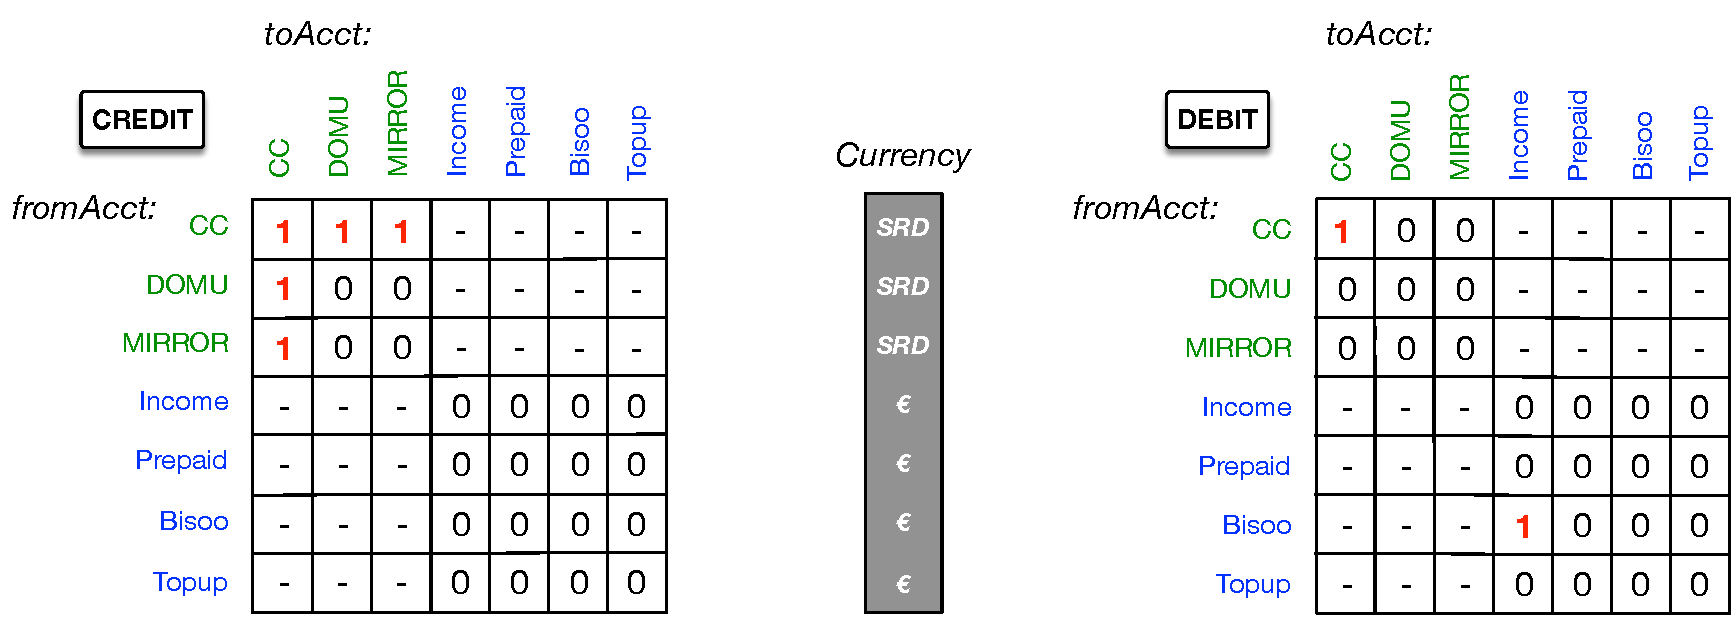
\includegraphics[width=16cm]{Figures/User_Acct_Connectivity}
\caption{\small\textbf{Account connectivity for user-initiated transactions: Test 2 in Figure \ref{fig:transactabilitywkflow}}}
\label{fig:User_Acct_Connectivity}
\end{figure}

\begin{figure}[H]
\vspace{-1cm}
\centering
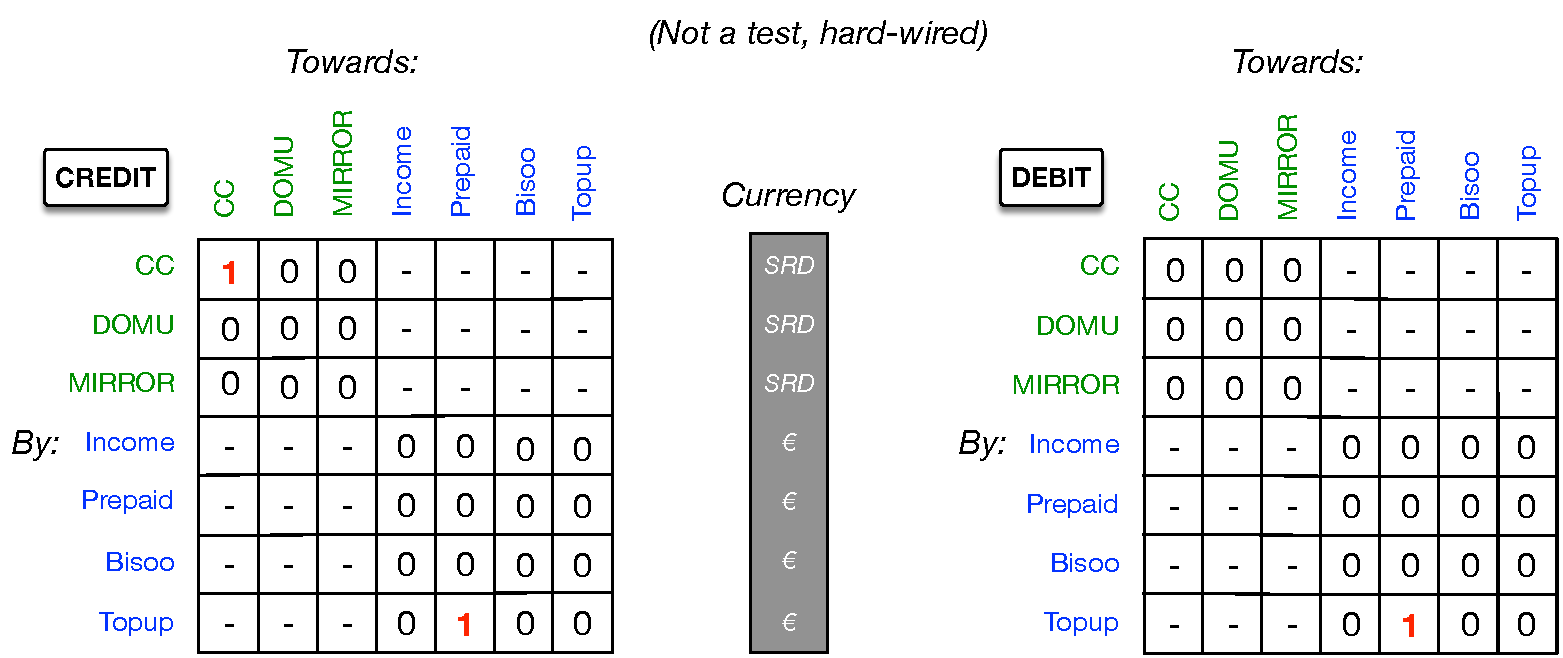
\includegraphics[width=16cm]{Figures/SysAdmin_Acct_Connectivity}
\caption{\small\textbf{Account connectivity for system-initiated transactions: Not a test, hard-wired. }}
\label{fig:SysAdmin_Acct_Connectivity}
\end{figure}

Figure \ref{fig:SysAdmin_Acct_Connectivity} shows a similar connectivity function for accounts that are controlled by $SysAdmin$. In this case, however, this function does not imply a transactability test since the permissions are hard-wired and SysAdmin does not need to test for transactability.

\subsection{User Transactability Functions}
\textbf{\small Note: this section has no bearing on the implementation, it is included to help interpret Figure \ref{fig:stack}.}

Figures \ref{fig:UTF1}-\ref{fig:UTF4} show a visualization of the interactions relevant to Layer 1 of Figure \ref{fig:stack}, filtered by the Account Connectivity constraints.

\begin{figure}[h]
\vspace{-0.5cm}
\centering
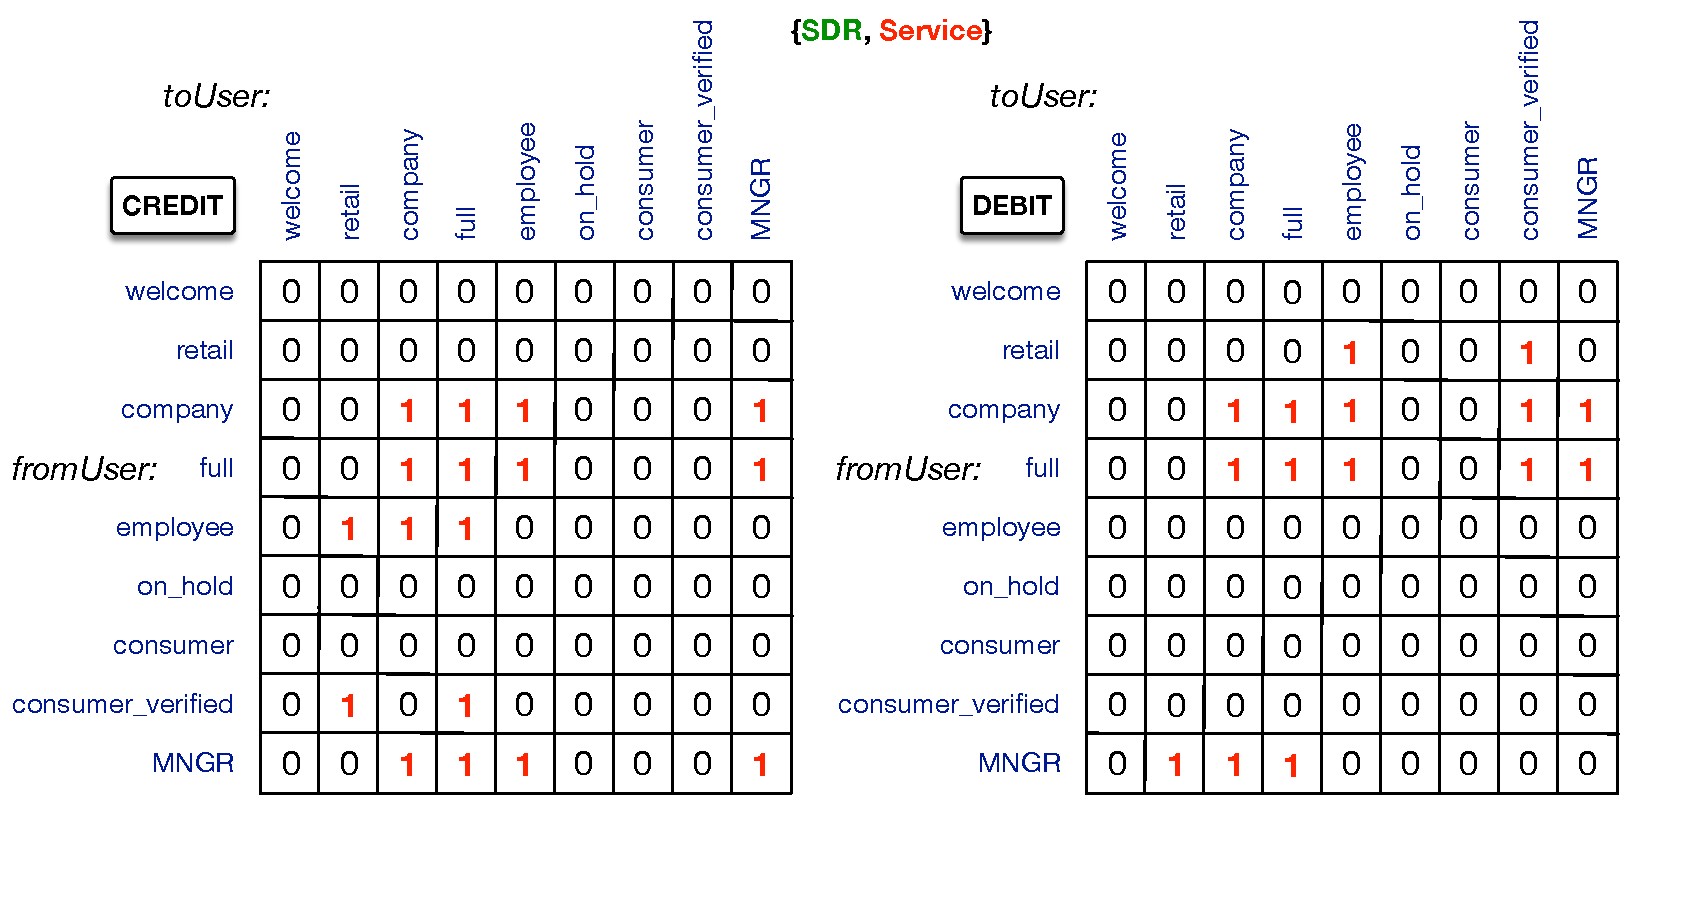
\includegraphics[width=17.5cm]{Figures/UTF1}
\caption{\small\textbf{User Transactability Function 1}}
\label{fig:UTF1}
\end{figure}

\begin{figure}[h]
\centering
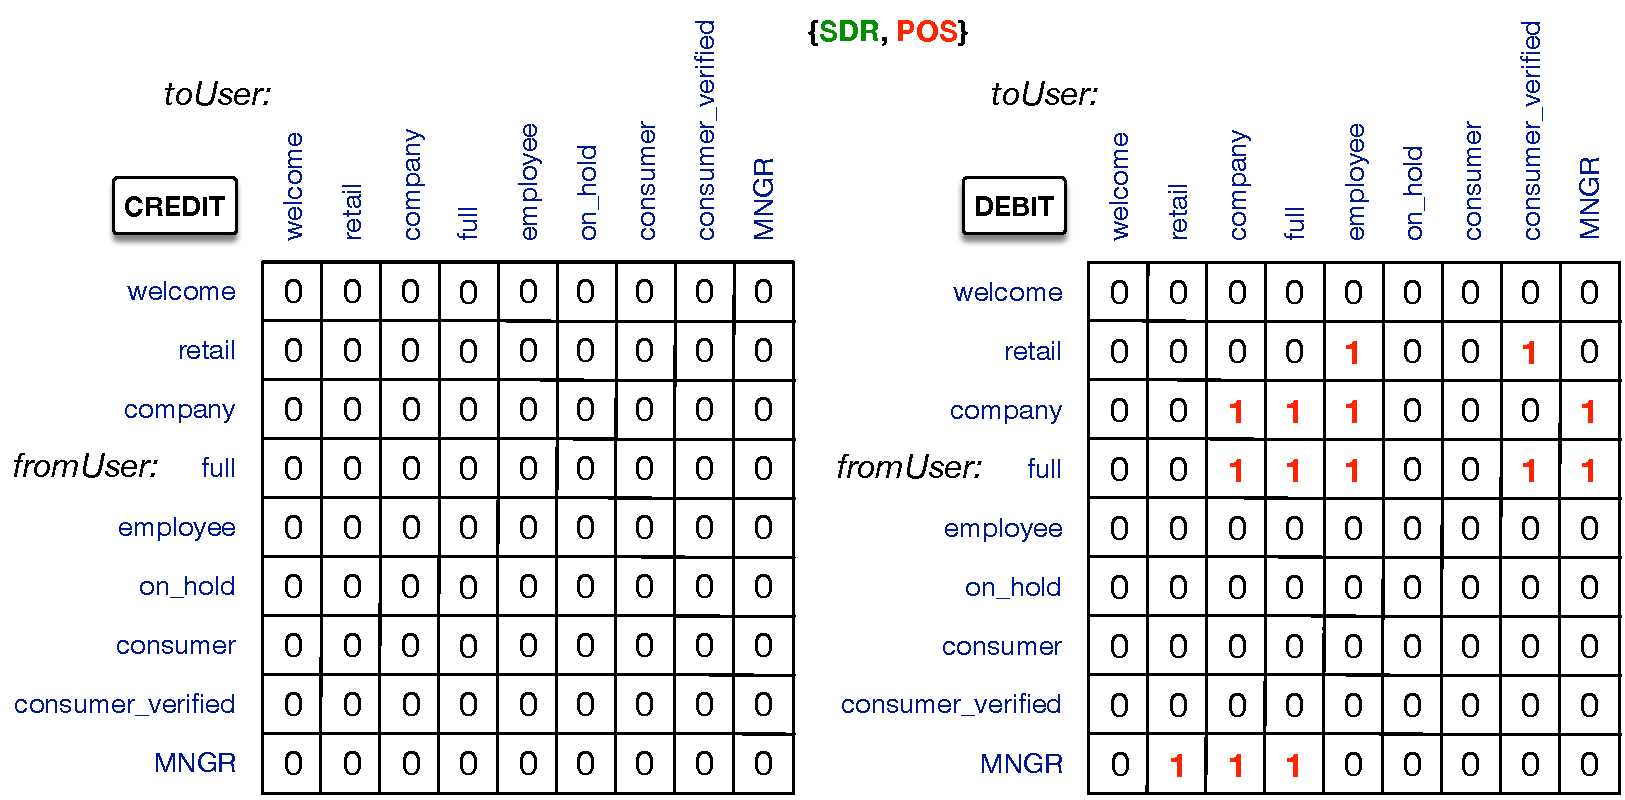
\includegraphics[width=17.5cm]{Figures/UTF2}
\caption{\small\textbf{User Transactability Function 2}}
\label{fig:UTF2}
\end{figure}

\begin{figure}[H]
\vspace{-0.5cm}
\centering
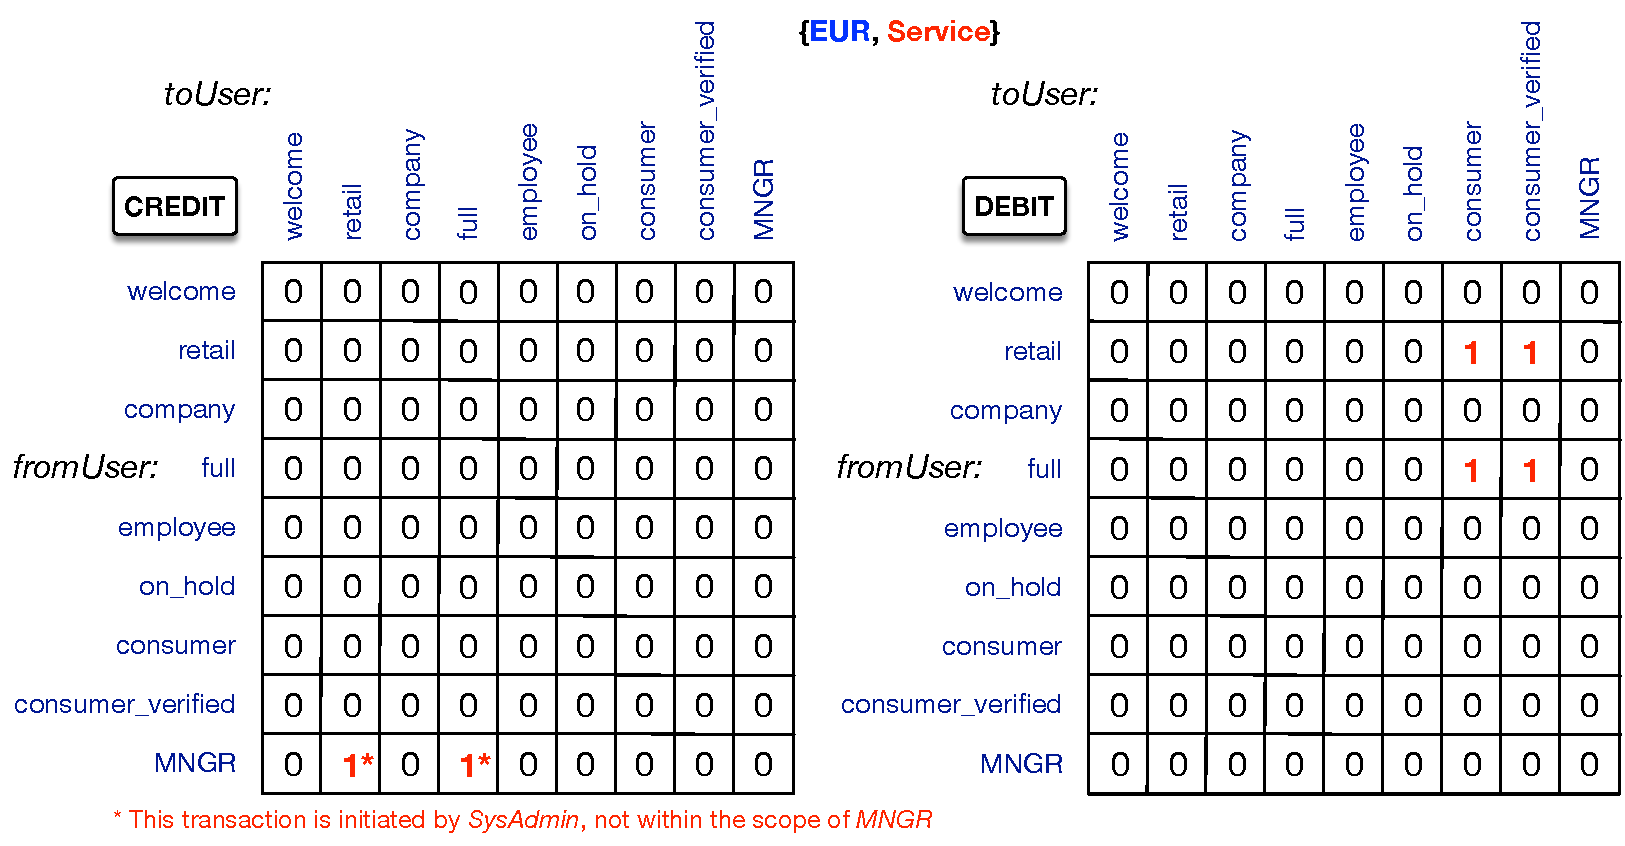
\includegraphics[width=17.5cm]{Figures/UTF3}
\caption{\small\textbf{User Transactability Function 3}}
\label{fig:UTF3}
%\vspace{-1cm}
\end{figure}

\begin{figure}[H]
\centering
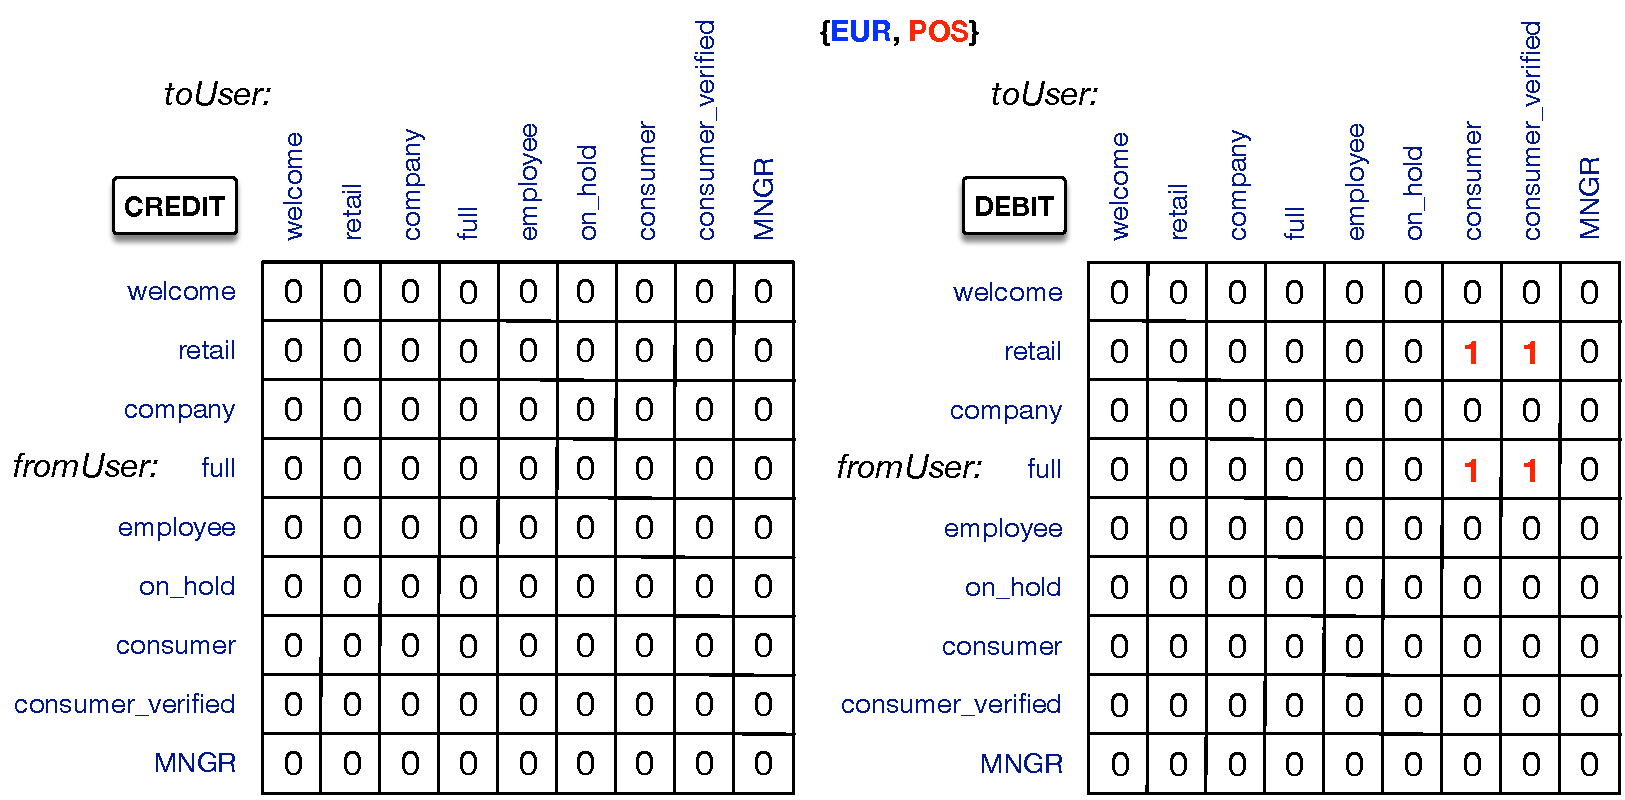
\includegraphics[width=17.5cm]{Figures/UTF4}
\caption{\small\textbf{User Transactability Function 4}}
\label{fig:UTF4}
\end{figure}



\subsection{Group Transactability Functions}
\textbf{\small Note: this section has no bearing on the implementation, it is included to help interpret Figure \ref{fig:stack}.}

The effect of the Transfer Types test together with the Account Connectivity test results in what we call the Group Transactability Function (GTF). Since there are 4 combinations of currency and channel, there are 4 different GTFs. There is no need to use them as an additional test, since they do not add anything new to Tests 1 and 2 of Figure \ref{fig:transactabilitywkflow}. However, it is still useful to include them here as another visualization of these first two tests of the Permissioning workflow, see Figures \ref{fig:GTF1}-\ref{fig:GTF4}.
\newpage

\vspace*{1cm}
\begin{figure}[h]
\centering
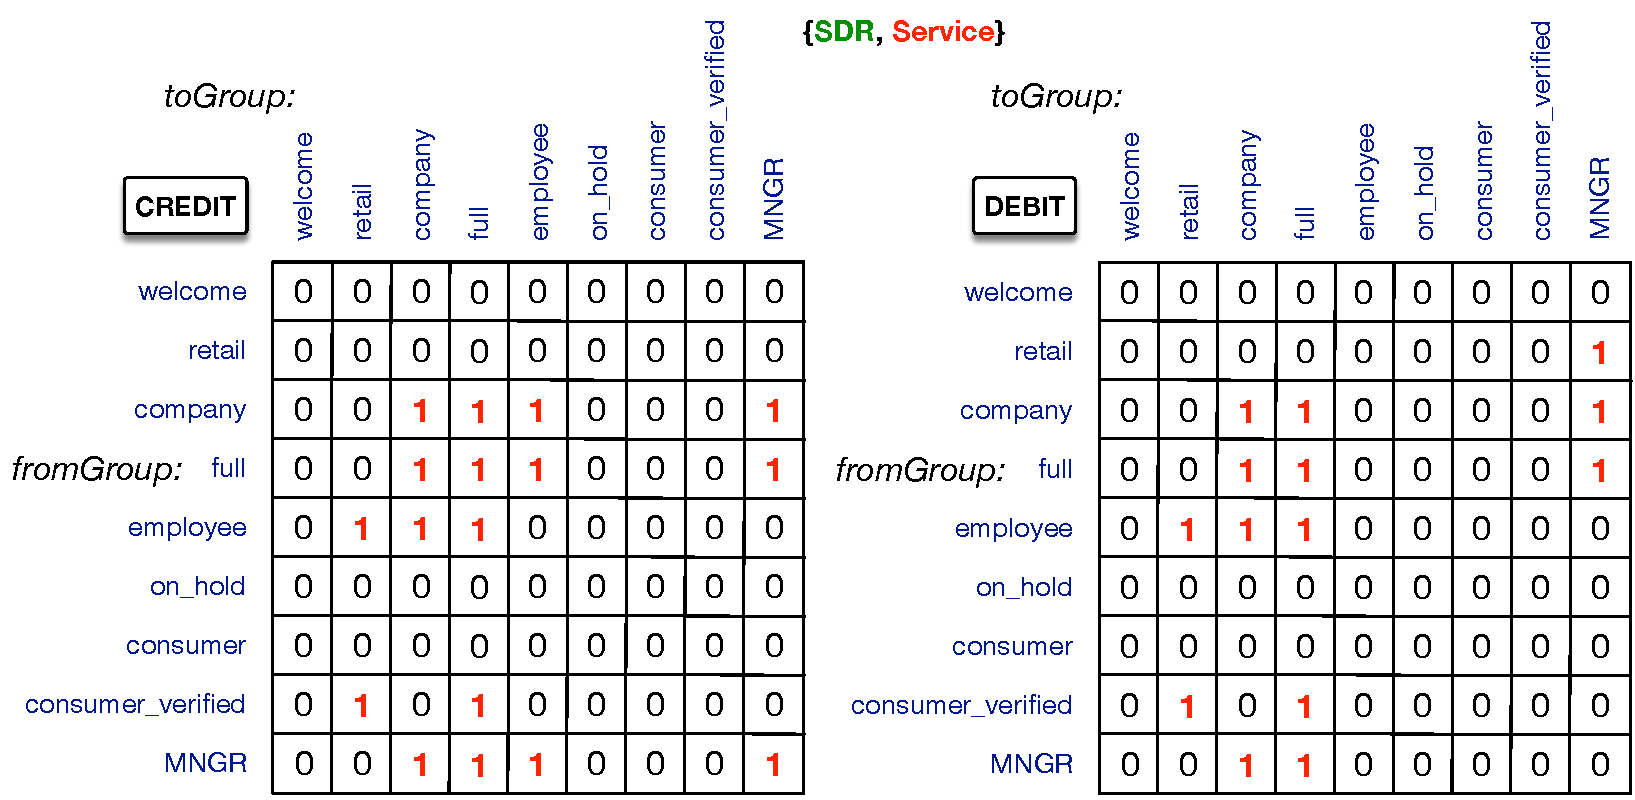
\includegraphics[width=17.5cm]{Figures/GTF1}
\caption{\small\textbf{Group Transactability Function 1}}
\label{fig:GTF1}
\end{figure}

\vspace*{2cm}

\begin{figure}[h]
\centering
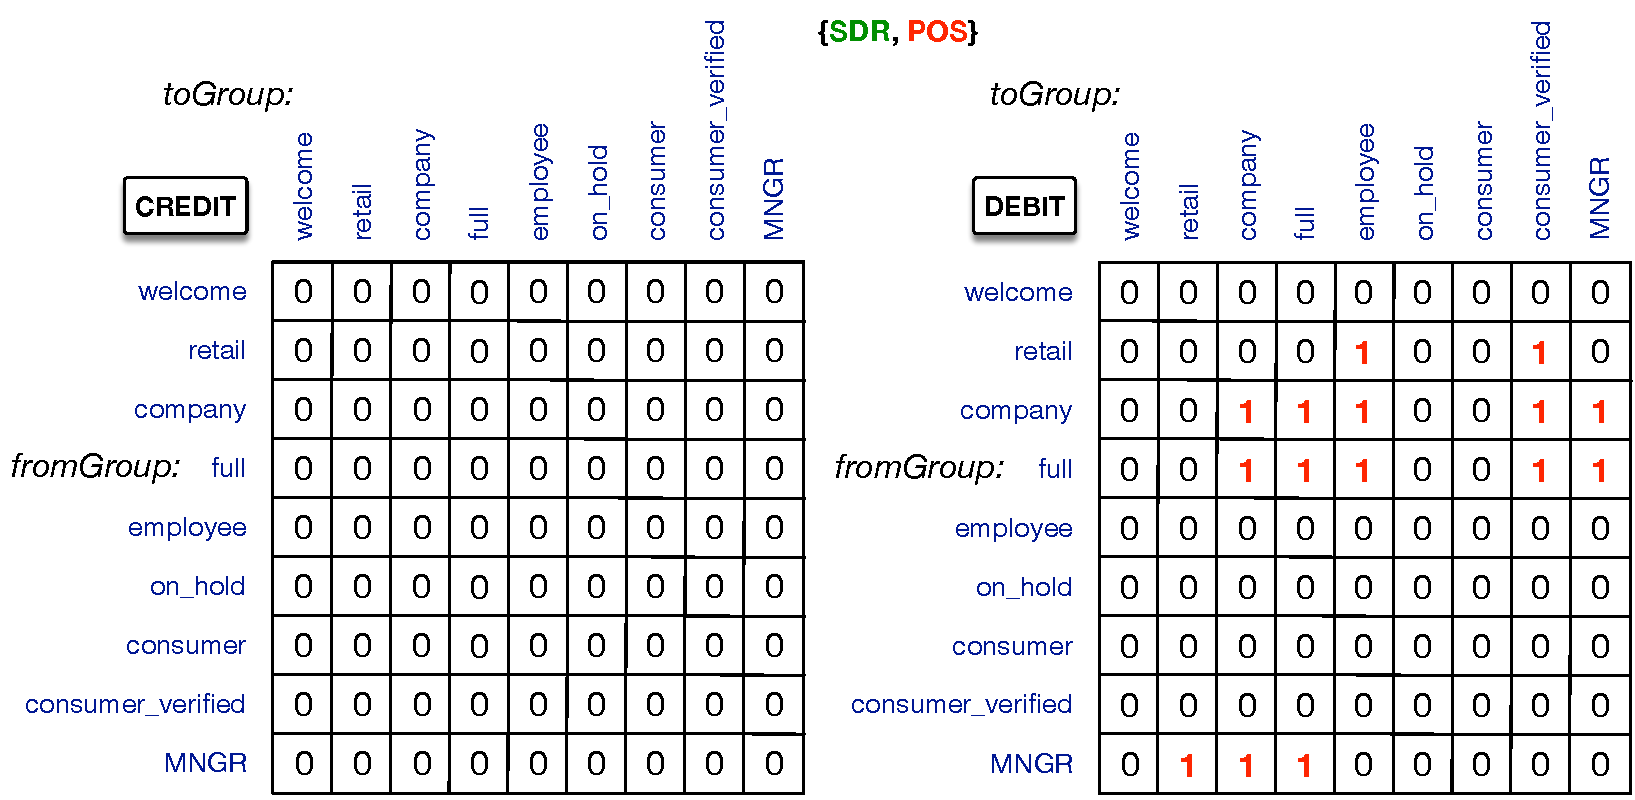
\includegraphics[width=17.5cm]{Figures/GTF2}
\caption{\small\textbf{Group Transactability Function 2}}
\label{fig:GTF2}
\end{figure}
%\vspace*{0.5cm}
\newpage

\begin{figure}[H]
%\vspace{-0.5cm}
\centering
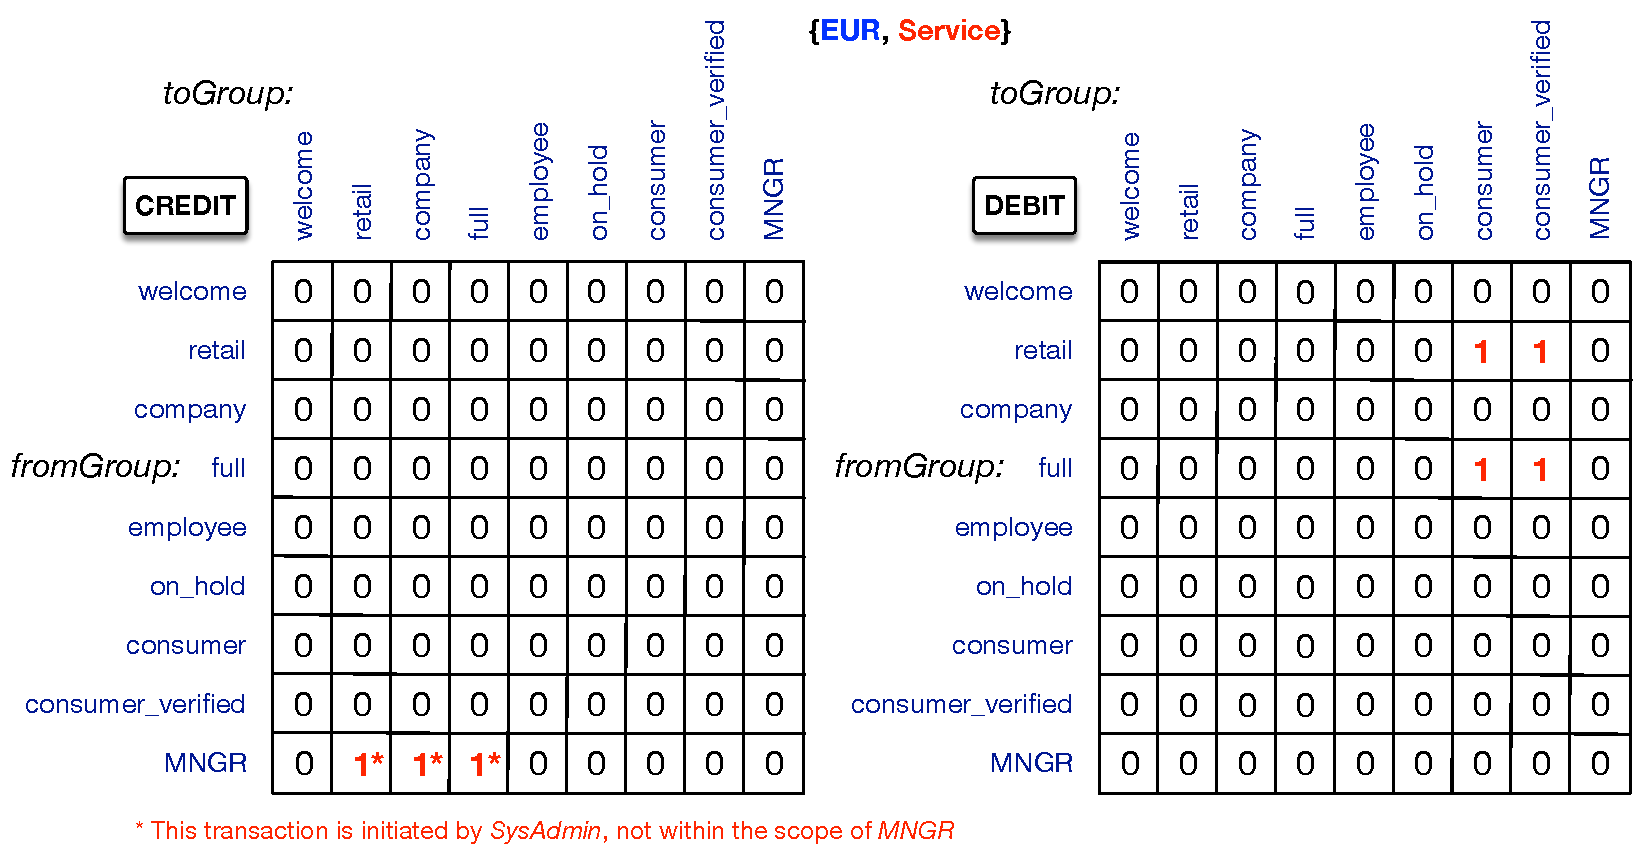
\includegraphics[width=17.5cm]{Figures/GTF3}
\caption{\small\textbf{Group Transactability Function 3}}
\label{fig:GTF3}
%\vspace{-1cm}
\end{figure}

\begin{figure}[H]
\centering
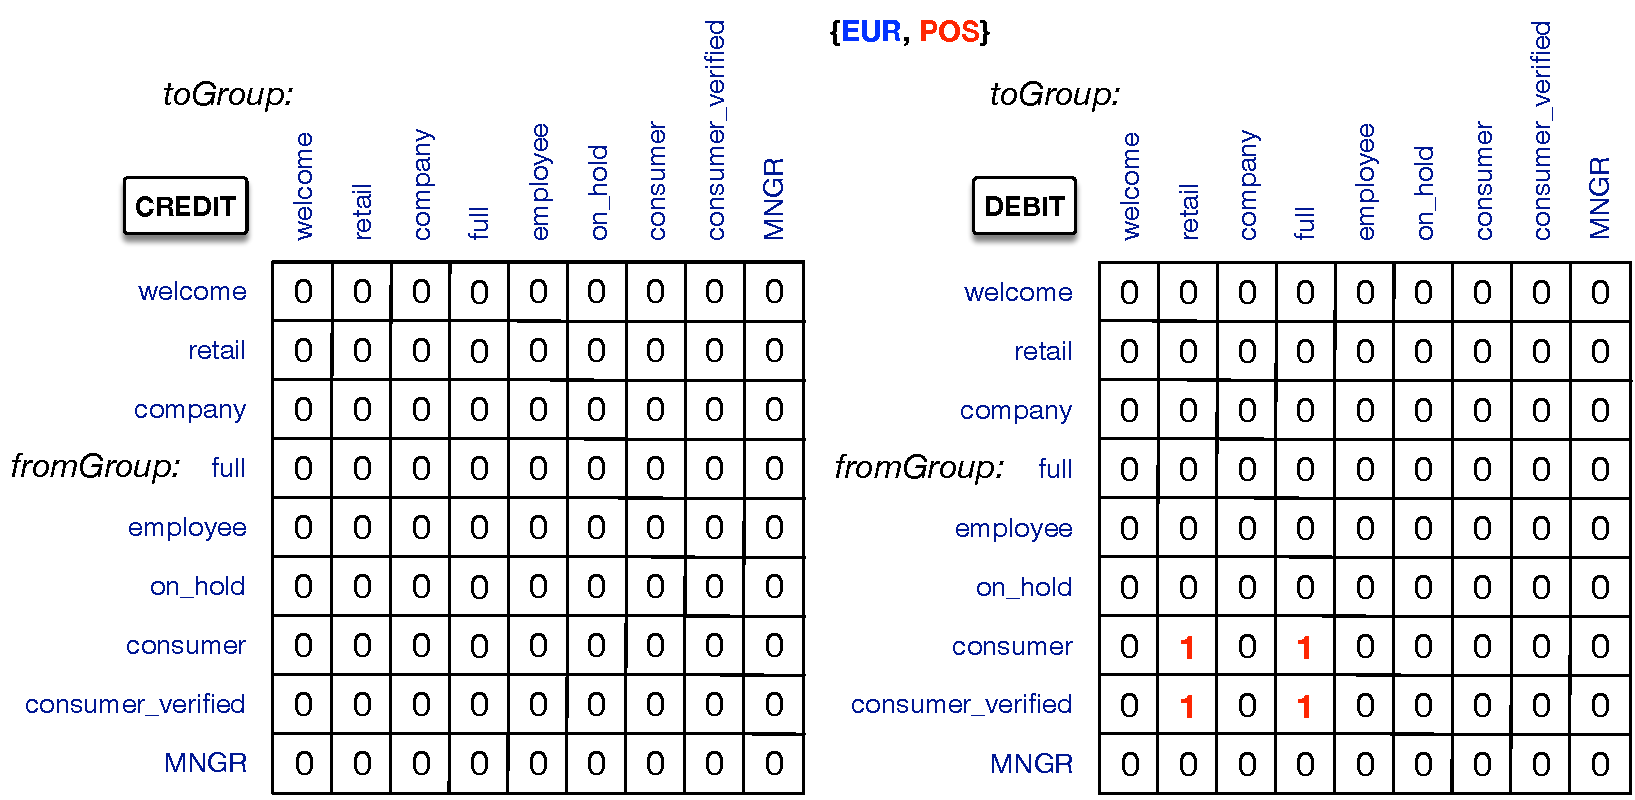
\includegraphics[width=17.5cm]{Figures/GTF4}
\caption{\small\textbf{Group Transactability Function 4}}
\label{fig:GTF4}
\end{figure}






\subsection{Transaction MetaData}

The transaction meta-data consists of only 1 memo message that is to be implemented as part of the transaction. It is not obligatory, i.e.\ the initiator of the transaction can leave it blank. The length is to be determined at the time of implementation but the assumption is that it is ``long enough'' to support a reasonable description of the transaction.

\newpage

\subsection{Account MetaData}
Tables \ref{tab:AccountMetaData1} and \ref{tab:AccountMetaData2} are also organized in terms of obligatory and optional meta-data, where the latter are modifiable by the user. At the implementation stage, for example, the modifiable fields can be included together with the profile meta-data. The fields that can be set by the user are indicated with an asterisk.

\begin{table}[H]
\begin{centering}
\small
{
\begin{tabular}{ r | c | l | l }
\hline
\textbf{Account}	& {\bf Account MetaData} & {\bf Type} & {\bf Description} \\
\Xhline{1.5pt}
			 & \emph{(Obligatory MetaData)}& & \\
\cline{2-2}
$CC$		& {\bf accountID}			&Integer	& Unique account identifier \\
			& {\bf memberID}			&String	& ProfileID of account owner \\
			& {\bf unit}					&String	& Account currency \\
			& {\bf balance}				&Double	& Account balance (positive or negative) \\
			& {\bf creditLimit}			&Double	& Credit limit (positive number) \\
			& {\bf creditLimitDate}		&DateTime & Date at which credit limit was set \\
			& {\bf availableBalance}		&Double	& $balance + creditLimit$ (positive number) \\
			& {\bf upperLimit}			&Double	& Upper balance limit (positive number) \\
			& {\bf availableCapacity}		&Double	& $capacity - saleVolume$ (positive number) \\
\cline{2-2}
			 & \emph{(Optional MetaData)}& & \\
\cline{2-2}
			& {\bf lowBalanceAlert$^*$}		&String	& Alert if $(creditLimit + balance) < lowBalanceAlert$ buffer \\
			& {\bf highBalanceAlert$^*$}		&String	& Alert if $(upperLimit - balance) < highBalanceAlert$ buffer \\
			& {\bf highVolumeAlert$^*$}		&String	& Alert if $(capacity - saleVolume) < highVolumeAlert$ buffer \\
\Xhline{1.5pt}
			 & \emph{(Obligatory MetaData)}& & \\
\cline{2-2}
$DOMU$		& {\bf accountID}			&Integer	& Unique account identifier \\
			& {\bf memberID}			&String	& ProfileID of account owner \\
			& {\bf unit}					&String	& Account currency \\
			& {\bf balance}				&Double	& Account balance (positive or negative) \\
			& {\bf creditLimit}			&Double	& Credit limit (positive number) \\
			& {\bf creditLimitDate}		&DateTime & Date at which credit limit was set \\
			& {\bf availableBalance}		&Double	& $balance + creditLimit$ (positive number) \\
\Xhline{1.5pt}
			 & \emph{(Obligatory MetaData)}& & \\
\cline{2-2}
$MIRROR$ 	& {\bf accountID}			&Integer	& Unique account identifier \\
			& {\bf memberID}			&String	& ProfileID of account owner \\
			& {\bf unit}					&String	& Account currency \\
			& {\bf balance}				&Double	& Account balance (positive or negative) \\
			& {\bf creditLimit}			&Double	& Credit limit (positive number) \\
			& {\bf creditLimitDate}		&DateTime & Date at which credit limit was set \\
			& {\bf availableBalance}		&Double	& $balance + creditLimit$ (positive number) \\
			& {\bf upperLimit}			&Double	& Upper balance limit (positive number) \\
			& {\bf availableCapacity}		&Double	& $capacity - saleVolume$ (positive number) \\
\cline{2-2}
			 & \emph{(Optional MetaData)}& & \\
\cline{2-2}
			& {\bf lowBalanceAlert$^*$}		&Double	& Alert if $(creditLimit + balance) < lowBalanceAlert$ buffer \\
			& {\bf highBalanceAlert$^*$}		&Double	& Alert if $(upperLimit - balance) < highBalanceAlert$ buffer \\
			& {\bf highVolumeAlert$^*$}		&String	& Alert if $(capacity - saleVolume) < highVolumeAlert$ buffer \\
\Xhline{1.5pt}
$Income$ 		& {\bf accountID}			&Integer	& Unique account identifier \\
			& {\bf memberID}			&String	& ProfileID of account owner \\
			& {\bf unit}					&String	& Account currency \\
			& {\bf balance}				&Double	& Account balance (positive or negative) \\
\Xhline{1.5pt}
\end{tabular}
}
\caption{\small\textbf{MetaData for $CC$, $DOMU$, $MIRROR$, and $Income$ accounts}\\
($^*$Indicates fields that can be modified by the user)}
\label{tab:AccountMetaData1}
\end{centering}
\end{table}

\begin{table}[H]
\begin{centering}
\small
{
\begin{tabular}{ r | c | l | l }
\hline
\textbf{Account}	& {\bf Account MetaData} & {\bf Type} & {\bf Description} \\
\Xhline{1.5pt}
			 & \emph{(Obligatory MetaData)}& & \\
\cline{2-2}
$Prepaid$ 	& {\bf accountID}			&Integer	& Unique account identifier \\
			& {\bf memberID}			&String	& ProfileID of account owner \\
			& {\bf unit}					&String	& Account currency \\
			& {\bf balance}				&Double	& Account balance (positive or zero) \\
			& {\bf creditLimit}			&Double	& Credit limit {\bf (Value can only be 0!)} \\
\cline{2-2}
			 & \emph{(Optional MetaData)}& & \\
\cline{2-2}
			& {\bf lowBalanceAlert$^*$}		&Double	& Alert if $(creditLimit + balance) < lowBalanceAlert$ buffer \\
\Xhline{1.5pt}
$Bisoo$ 		& {\bf accountID}			&Integer	& Unique account identifier \\
			& {\bf memberID}			&String	& ProfileID of account owner \\
			& {\bf unit}					&String	& Account currency \\
\Xhline{1.5pt}
$Topup$ 		& {\bf accountID}			&Integer	& Unique account identifier \\
			& {\bf memberID}			&String	& ProfileID of account owner \\
			& {\bf unit}					&String	& Account currency \\
\Xhline{1.5pt}
\end{tabular}
}
\caption{\small\textbf{MetaData for $Prepaid$, $Bisoo$, and $Topup$ accounts}\\
($^*$Indicates fields that can be modified by the user)}
\label{tab:AccountMetaData2}
\end{centering}
\end{table}

\section{Account Limit Tests}
The account limit tests are specified abstractly in D2.1. In the context the description of this chapter, which is closer to the implementation, they are fairly obvious by looking at Figures \ref{fig:accountLimitsCC} and \ref{fig:accountLimitsPrepaid}. The important thing is that they need to be enforced \emph{before} a transaction is completed. If one of the tests fails the transaction is not executed and the user must be alerted.

The alerts, on the other hand, can be issued \emph{after} a transaction that came close to a limit but did not cross it, if the resulting balance or sale volume exceeds the buffer limits.




























\chapter{Introduction to the CoreASIM Language, Interpreter, and ICEF}
\label{ch:CoreAsimIntro}

\vspace{-1cm}
\begin{center}
Eduard Hirsch
\end{center}

In this chapter an overview of the used technologies for running the INTERLACE Specification is given. At the beginning a quick start description is provided in order to jump right into the execution of the model.

Further details which are enabling the Abstract State Interacting Machines (ASIM) specifications to be executed are discussed and why this possible in a simple and stable manner.

\section{Quick Start Vagrant}
\label{sec:quick-start-vagrant}

There are two base environments available. One based one docker and one based on vagrant. The focus shifted from the vagrant environment which can be downloaded at github\footnote{https://github.com/InterlaceProject/ASIMVagrantEnvironment} to a docker based version which is explained in section \ref{sec:quick-start-docker}. Nevertheless, for developer preferring vagrant, the setup will be still explained.

The vagrant definition provides a running environment for executing the INTERLACE ASIM definitions. During the provisioning process an ubuntu vagrant box is set up which installs the necessary components on that box. It is cloning and building the ICEF framework\footnote{https://github.com/biomics/icef} as well as the ASIM Specification\footnote{https://github.com/InterlaceProject/ASIMSpec} into the data directory where it is finally ready for usage.

\subsection{Prerequisites}

Download and install the following software products:

\begin{itemize}
	\item Virtual Box: https://www.virtualbox.org/
	\item git: https://git-scm.com/downloads
	\item vagrant: https://www.vagrantup.com/
\end{itemize}

\subsection{Clone Environment}

To clone the ASIM vagrant environment from github into a directory git can be utilized:

\begin{lstlisting}
	git clone https://github.com/InterlaceProject/ASIMVagrantEnvironment.git
\end{lstlisting}

\subsection{Execution}

Once all software components are installed and the vagrant definitions are cloned it is possible to call

\begin{lstlisting}
	execute.sh
\end{lstlisting}

from the main directory in order to let the INTERLACE specifications run. Note: when using Windows it is necessary to start that command within git-bash which needs to run in elevated admin mode (right click $\rightarrow$ start as administrator).

On the very first execution the script is provisioning a virtual machine based on ubuntu by calling \texttt{vagrant up} which may take some time. Consecutive calls will be much faster. A detailed description explaining the precise process is covered in section \ref{sec:exec-env-model-details}.

Once the execution is started it will run until it is stopped by pressing \textbf{ctrl + c} or by calling

\begin{lstlisting}
	stop.sh
\end{lstlisting}

from any other console window.

\section{Quick Start Docker}
\label{sec:quick-start-docker}

The docker project at github\footnote{https://github.com/InterlaceProject/ASIMDockerEnvironment} is also based on virtualization like the vagrant environment but emphasizing \textit{Operating System} instead of \textit{Hardware virtualization}\footnote{https://www.docker.com/what-container\#comparing}.

\subsection{Prerequisites}

\begin{itemize}
	\item install docker
	\item install git (including git bash for windows)
\end{itemize}

On Linux machines it is important to add the current user to the docker group in order to manage docker container and images. Otherwise all further explained commands need to be executed as root or with sudo.

For Windows machines use \textit{git-bash} to execute the commands described in the following sections.

\subsection{Before First Execution}

In order to configure the environment it is necessary to call the following script:

\begin{lstlisting}
	./configure
\end{lstlisting}

This will generate a docker container image called \textit{asim} where all the necessary frameworks are build and prepared for execution of the specifications. The ICEF framework as well as the ASIM model specifications are cloned outside of the container to simplify development.

\subsection{Execute Specification}

The container image \textit{asim} created during the configuring step can be started by calling

\begin{lstlisting}
	./execute
\end{lstlisting}

A container started in this way is called \textit{active\_asim} and running all the necessary steps like starting an ICEF manager as well a ICEF brapper to run the ASIM specifications.

Like the vagrant environment a running execution may be stopped by pressing \textbf{ctrl + c}.

\section{Execution Environment Stack}
\label{sec:exec-env-stack}

Independent of the used virtualization techniques a consistent base system is used. So both docker as well as vagrant are provisioning a Linux based operating system using an Ubuntu 16.04 LTS (Long Term Support) distribution.
That consistent, stable and reliable structure will be important later when considerations about provability as well testability come into place. That design provides always the same preconditions and everybody executing or testing against the specifications will receive the same results.

\subsection{Software Stack}
\label{sec:env-exec-stack-software-stack}

The Ubuntu 16.04 LTS distribution is enhanced and updated according to the needs of an ASIM executing machine as well as to the needs of developers working with that virtual system. To be more specific the following components are installed during the provisioning process:

\begin{itemize}
	\item curl $\rightarrow$ Tool for querying REST resources (used for downloading package resources)
	\item nodejs $\rightarrow$ JavaScript engine including the package manager npm (running the Manager Component of ICEF)
	\item build-essential $\rightarrow$ Packages needed to compile a debian based package (used for building the project sources)
	\item maven $\rightarrow$ Java build and packaging tool (used for building the project sources)
	\item vim $\rightarrow$ Well known U/Linux editor (for development purposes)
	\item git $\rightarrow$ Distributed Version Control System (downloading source repositories from GitHub)
	\item Java 8 $\rightarrow$ Programming Language used for coreASIM base system implementation (running ASIM instances)
\end{itemize}

\subsection{Provisioning Process}

The provisioning process can be separated into 3 steps which are executed when \textit{.\/configure} for docker or \textit{vagrant up} for vagrant is called from the command line:

\begin{enumerate}
	\item Download ASIMSpec and ICEF from GitHub
	\item Install of software packages mentioned in section \ref{sec:env-exec-stack-software-stack}
	\item Build ICEF framework and prepare virtual machine for execution
\end{enumerate}

For development purposes the ASIMSpec as well as the ICEF framework are cloned into directories which are available from the host machine and the virtual guest machine. This is necessary because then it is possible to directly edit the source or debug from outside and execute the code from within the container. Consequently it is not necessary to copy the code into the container when changes where done.

For \textbf{Vagrant} a shared folder is configured over the vagrant file shown here

\begin{lstlisting}
	...
	config.vm.synced_folder "./data", "/vagrant-data"
	...
\end{lstlisting}

is referring to the fact that on the host system the folder \textit{data} is used and on the guest system a folder \textit{vagrant-data} is mounted. Those folder are shared and thus containing the same content. Additionally during provisioning a symbolic link in the home directory is created called project (\textit{/home/ubuntu/project}) which is linking the mounted root folder /vagrant-data.

When the virtual machine is stopped the data directory on the host is kept and can be still manipulated or executed (of course only if the framework dependencies are installed on the host as well).

For \textbf{Docker} we need to first clone all GitHub sources to the host machine and can only then share the files into the guest container by using the command line option "-v"

\begin{lstlisting}[language=bash]
	docker run -v "$1/ASIMSpec:/home/ASIMSpec" \
	           -v "$1/icef:/home/icef" \
	           --name active_asim -it asim /$2
\end{lstlisting}

This line is part of the script \textit{scripts/runDocker.sh}. \$1 here stands for the local directory of the environment and \$2 is normally defaulted to the main execution script started inside the docker container. Important to note is that the \textit{ASIMSpec} folder of the host machine is shared into \textit{/home/ASIMSpec} of the docker container and the \textit{icef} directory is shared into \textit{/home/icef}.

\subsection{Execution}
\label{sec:env-exec-stack-exe}

The execution stack in figure \ref{fig:icef-intro-asim} shows where a ICEF specification is transmitted to for it to be executed. The details will be covered in section \ref{sec:icef-intro}. In this part of the document, however, we will take a look at how and which services are started.

Due to limitations of the ICEF framework it is currently not possible to cleanly shut down a running ICEF simulation with several running ASIM instances. Therefore both environments have to start and stop all services for every execution in order to grant a correct execution set-up.

\subsubsection{Start Services Processes}: Both environments offer a script (\textit{execute(.sh)}) to be called from the host system and one from within the virtualized machine (\textit{executeASIMSpec.sh/executeOnGuest.sh}). Whereas the script on the virtualized system only differ in directory references the outside scripts are need to handle different things as one script is dealing with docker and the other with vagrant.

In detail Docker can immediately start the servers and run the script inside the container whereas vagrant needs add an additional step if the virtual machine is not up and running yet. Thus vagrant

\begin{enumerate}
	\item is trying to start the server processes and submit the specifications
	\item if the first step failed is checking for the virtual machine if it is running and if not it tries to restart the virtual machine
	\item if the restart has been successful the first step will be retried.
\end{enumerate}

When now focusing on the first step which is basically the same on both environments it can be discussed in detail how the process is continued. So on the guest system we are first running a so called \textit{CASIMA} which is short hand for coreASIM-Manager \ref{sec:icef-intro}. This manager takes care about ASIM states, scheduling and also acts as messaging backbone.

Next a second service process is started. The service is a wrapper for the coreASM implementation and its name is Brapper (BIOMICS wrapper). This Brapper service executes enhanced ASM code named BSL that offers additional language primitives specifically designed during the BIOMICS project. Those features mainly include interaction features used to model biochemical systems, nevertheless, and actually because of that they are also suitable for decentralized and distributed computer system.

When a Brapper is going to be started it needs to be register at a manager instance. As described in section \ref{sec:icef-intro} it is possible to start multiple Brappers. Once a simulation is submitted to the manager, the manager is distributing the different simulations including their ASIMs to different Brapper services for executing them there trying to spread the load equally.

For the sake of simplicity the environment starts only one Brapper by default. In the final implementation it'll be possible to configure the number of Brappers used for execution.

\subsubsection{Submit ICEF definition file}: Finally after the service processes are running it is possible to submit a specification file to the manager. This is done by the executing bash script which is calling a  nodejs client:

\begin{lstlisting}
	...
	node loadICEF.js $project/ASIMSpec/run.icef localhost 9090
	...
\end{lstlisting}

The above listing uses a \textit{\$project} variable containing the path of ASIMSpec to find the icef specification. By convention the icef definition file of the ASIM Specifications is called \textit{run.icef} to clearly identify the entry point for the environment.
The last two parameters for the script are host as well as port where the manager services is running and waiting for requests.

\subsection{Development}
\label{sec:development}

For developing new simulations it is important to have a proper development environment. There are existing many IDE/Tool/Debuggers for Java and JavaScript which are used for Brapper, Manager or coreAS(I)M plugin development but there are only limited IDE choices for implementing AS(I)Ms.

For the public Integrated Development Environment Eclipse, developers of the ICEF framework have adopted the coreASM plugin for supporting the additional language primitives. Thus for working with ASIM implementations of INTERLACE you ideally DO NOT download the coreASM package which is available at the market place of Eclipse. The adopted plugin working with the new language elements is provided by the ICEF framework but is needed to build and imported manually into Eclipse.


\textbf{Import/Install of the IDE Eclipse plugin for coreASIM}
\begin{description}
	\item[Build Framework] For adding the ASIM plugin to Eclipse it is required to build and install the coreASIM plugin manually first because it is not downloadable from the Eclipse marketplace and only available as source version delivered with the ICEF framework and part of the coreASIM engine. Building and installing can be done by calling
	\begin{lstlisting}
		cd icef/coreASIM/org.coreasim.parent && mvn package install
		cd icef/coreASIM/org.coreasim.eclipse && mvn package install
	\end{lstlisting}
	Note that the icef directory is placed on different folders in the two environments!
	
	\item[Install Plug-In Development Environment in Eclipse] To install the ASIM Plug-in it is necessary to first add another Plug-in called Eclipse PDE (Plug-In Development Environment) from the marketplace for the current Eclipse installation or get a distribution which already contains that Plug-in.
	
	\item[Import Plugin as Project] Next the plugin needs to be imported to the workspace which can be done in Eclipse using the import wizard. To reach the wizard go to "File" $\rightarrow$ "Import...", search for "Existing Projects into Workspace" and click to get to "Import Project"-Window. Then click "Finish" to import the project.
	
	\item[Dry-Run Eclipse with coreASIM-Plug-In] This optional step can be done to check if the Plug-In is working correctly. For that it is necessary to right click the imported eclipse project and go to "Run As" $\rightarrow$ "Eclipse Application". Then a second Eclipse instance is started but this time a new tab should appear named "coreASIM" as well as when opening a file with extension \textit{casim} the ASIM definition should be syntax highlighted.

	\item[Enable the Plug-In] If the (optional) dry-run has been successful the export wizard will export the Plug-In into the running Eclipse installation by opening "File" $\rightarrow$  "Export" then choosing "Deployable Plug-ins and fragments" in the new Dialogue. The window which is opened next will offer to export fragment  \textit{org.coreasim.eclipse} by selecting the check box beside. Before clicking finish the combo box "Install into host" has to be chosen.
	
\end{description}

When finishing these steps on restart Eclipse offers a new tab in the top menu bar called "CoreASIM".

\textbf{Note on the installation}: When using the \textit{docker}-Environment you could skip the first step \textbf{Build Framework}, because all the necessary build steps are covered by the initial configuration script. Also a separate installation of the Eclipse Plug-In Development Environment (PDE) might omitted because it usually comes in a bundle with most standard J2EE installations of Eclipse.

\textbf{Notes on the Docker environment}
\label{sec_inner:note-docker}

Normally the ASIM Specifications are started by calling \textit{execute} from the main directory which is starting a script which will run the services and sent the ICEF definition. When stopping the container it instantly goes back to his original state before execution. Only the shared directories ASIMSpec and icef keep changes.

If it is necessary or convenient, like if the host is missing development packages (e.g. maven, nodejs, ...) which are available inside the container, it is possible to work from within the container by calling

\begin{lstlisting}
	./execute /bin/bash
\end{lstlisting}

which starts the docker container, runs a bash shell, keeping the STDIN open and connect a pseudo TTY. In this way it is possible to work with that bash shell, similar to connecting to a machine over SSH.

\section{ICEF - The Interaction Computing Execution Framework}
\label{sec:icef-intro}

The interaction framework is wrapping the original coreASM framework in order to extend it and giving it the capabilities to execute concurrent and distributed. It has been developed in a project called BIOMICS and financed by the European Commission.

\textbf{This wrapping took place on three levels:}

\textbf{First} the interpreter coreASM had to be extended supporting additional languages primitives as well as communications features. Here BSL replaces ASM as a new language having a new interpreter coreASIM.

\textbf{Second} a place has been created were the now so called Abstract State Interaction Machines (ASIMs) take over and are able to execute in parallel. This environment is called Brapper (short for BIOMICS Wrapper).

\textbf{Third} a central server called manager takes care handling distributed Brapper instances dealing with message and scheduling issues.

Technology wise coreASIM changes the coreASM implementation in Java. Brappers are written in Java as well but the managers are coordinating the Brappers using nodejs and therefor written in JavaScript.

\subsection{Framework Stack}

Next, the framework stack of ICEF in terms of the INTERLACE implementation is described more detailed. In figure \ref{fig:icef-intro-asim} the stack can be viewed in different levels of granularity.

As a stable base for the INTERLACE execution environment stack a Linux based system, Ubuntu 16.04 LTS, has been chosen. A LTS (Long Term Support) version is important to be sure to have a reliable platform which is maintained by the distributor for long time. Ubuntu publishes those version every two years and promises a maintenance duration of five years\footnote{https://www.ubuntu.com/info/release-end-of-life}.

After installation of the software described in \ref{sec:env-exec-stack-software-stack} and building the icef components the framework is ready. When the components are started it is possible to transmit a running definition, called ICEF JSON file.

In listing \ref{lst:icef-json-spec} it is possible to see how the specification for the simulation is looking like. Side note: A definition for the client here is not given because the client which is sending credit, debit or other requests is spawned and destroyed on demand by the scheduler ASIM.

\begin{lstlisting}[language=json,firstnumber=1,caption={ICEF Json Specification for Interlace},captionpos=b,label=lst:icef-json-spec]
{
   "id": "interlace", 
   "schedulers": [
       {
	   "file": "casim/scheduler.casim",
	   "start": true
       }
   ], 
   "asims": [       
       {
           "file": "casim/server.casim",
           "start": true
       }
   ]
}
\end{lstlisting}

Detailed description on parameters and options of the JSON ICEF specifications can be found in deliverable D5.2 \cite{BIOMICSD52} of the BIOMICS project.

The implementation idea here is to have a central server which is taking over the various requests from the clients. A scheduler will take care when and what is exactly running. As a second task the scheduler will also spawn new clients which send or receive information/inquiries to other components, but mainly to the server.

\textbf{The Submission Process} of the \textit{run.icef} works the following way:

\begin{description}
	\item [Loading and parsing of the ICEF-File] is initializing the process. Using that specification file a node.js components transmits the structure to the manager server process which acts as the central managing and communication node.
	\item [Manager Simulation] is started on the manger service process. Then the service is registering a new simulation and all components necessary for managing the different resources like messaging.
	\item [Distribute ASIMs] When simulations are initialized requests are sent to one or more Brappers in order to start up the actual running instances of the ASIM-agent.
	\item [Run ...] finally when all ASIM instances are running the simulation is successfully executing till stopped from outside or by a problem during execution.
\end{description}

\begin{figure}[htbp]
  \centering
  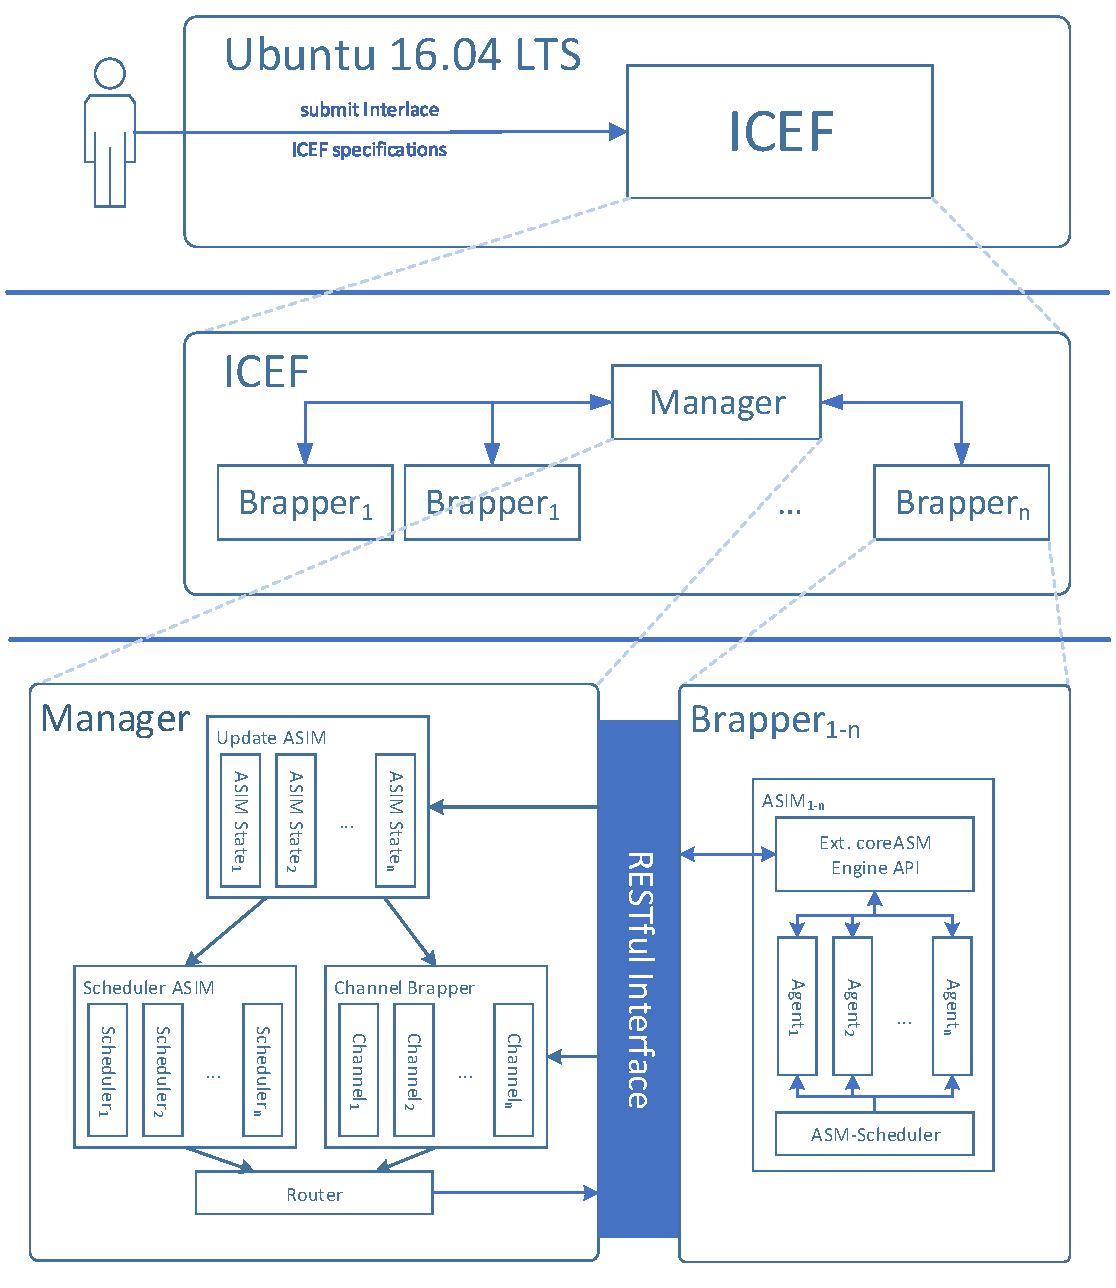
\includegraphics[width=1.0\textwidth, clip, trim=1mm 1mm 1mm 1mm]{Figures/environment_asim}
  \caption{ASIM Execution Environment Overview}
  \label{fig:icef-intro-asim}
\end{figure}

Figure \ref{fig:icef-intro-asim} illustrates on different level of detail which components and services are active and necessary to proved the previously described process running a ASIM simulation and in case of INTERLACE the model specifications.

\subsection{coreASIM}
\label{sec:coreasim-details}

The very core of the Interaction Computer Execution Framework (ICEF) is an engine which has been developed by different people at different universities \footnote{https://github.com/CoreASM/coreasm.core/wiki/About\-CoreASM} and implements a language called ASM. This language is based on Abstract State Machines \cite{BoergerStaerk2003} which is used as a method for high-level system engineering, design and analysis. This engine which is called coreASM got enhanced by the BIOMICS project in order to simulate computer interactions on a logic based programming language.

The resulting engine was called coreASIM including the missing interaction features \cite{BIOMICSD42}\cite{BIOMICSD52} and replaces language ASM by the BIOMICS Specification Language (BSL). The changes from the original framework also comprise of:

\begin{itemize}
	\item interactions possibilities
	\item abstract shared storage
	\item mailing system
	\item full scheduler
	\item interpreter enhancements
\end{itemize}

As this document offers only an overview only the most important implementations are described here, namely the mailbox and the scheduling system. \textbf{The mailing system} can easily be used and can be described as follows:

\begin{minipage}{1.0\textwidth}
An ASIM $asim_1$ can send a message to another ASIM $asim_2$ by using the send message rule.\nopagebreak
\begin{lstlisting}[language=bsl]
	send Element to "asim_2" with subject "a subject"
\end{lstlisting}

Where the \textit{Element} can be of any element location used in ASIM language space. Even for example \textit{programm(self)}.
\end{minipage}

\textbf{The scheduler} has the ability to coordinate different local agents in a way that they act in a predictable and appropriate way. Like the coreASM scheduler coreASIM implements a mechanism controlling at a higher level. At the beginning of each running step, a scheduler takes the defined scheduling policy and is using it to determine a set of local agents which will be signaled to run their program. There are different BSL constructs to do so. Here are two examples:

\begin{lstlisting}[language=bsl]
	forall a in Agents do schedule a
\end{lstlisting}

Which tells the scheduler to run all agents in \textit{Agents}. If a in contrary a single agents should be selected based on a condition $cond$ met by agent $a$, the respective rule might look like this:

\begin{lstlisting}[language=bsl]
	choose a in Agents with cond(a) do schedule a
\end{lstlisting}


\section{Model Execution Environment Details}
\label{sec:exec-env-model-details}

This section will describe and elaborate about the docker-Environment in depth, how the scripts are preparing/building the environment and what is needed to finally execute the Interlace Model Specifications described by \textit{run.icef} of the ASIMSpecs.

Starting from the directory structure in Figure \ref{fig:docker-env-file-struct} a detailed picture will be drawn. Due to performance and  development purposes docker has been chosen in favor of the vagrant-Environment. Although scripts of the two environments are quite similar focus will be laid on docker.

\tikzstyle{every node}=[draw=black,thick,anchor=west]
\tikzstyle{selected}=[draw=red,fill=red!30]
\tikzstyle{optional}=[dashed,fill=gray!50]
\begin{figure}[htbp]
\centering
\begin{tikzpicture}[%
  grow via three points={one child at (0.5,-0.7) and
  two children at (0.5,-0.7) and (0.5,-1.4)},
  edge from parent path={(\tikzparentnode.south) |- (\tikzchildnode.west)}]
  \node {Docker\ Environment}
    child { node {configure}}		
    child { node {Dockerfile}}
    child { node {execute}}
    child { node {README.md}}
    child { node [selected] {scripts}
      child { node {asimrc}}
      child { node {buildICEFDocker.sh}}
      child { node {executeASIMSpec.sh}}
      child { node {runDocker.sh}}
    };
\end{tikzpicture}
\caption{Docker Environment File Structure}
\label{fig:docker-env-file-struct}
\end{figure}

\subsection{Environment Configuration}

A crucial step for initializing a proper environment is the so called provisioning of the docker-Environment. The \textit{configure} bash script is handling this process. The script is prepared to be executed on Mac, Windows (using git bash) and Linux. It is tested with docker community edition. It is not yet tested with boot2docker environment and therefor might have problems there.
\chapter{CoreASIM Implementation of the INTERLACE Business Logic}
\label{ch:CoreAsimImplementation}

\vspace{-1cm}
\begin{center}
Eduard Hirsch, Maria Luisa Mulas and Paolo Dini\footnote{Eduard performed the lion share of the implementation and all of the writing of this chapter; Maria Luisa supported the implementation and the trouble-shooting; Paolo did no implementation but thoroughly edited this chapter to mazimize clarity of expression.}
\end{center}

This chapter describes the ASIM implementation performed according to the specification of Deliverable D2.1 \cite{INTERLACE_D21}, as well as the refinement of the requirements specification presented in Chapter \ref{ch:UpdateBLS} and restated formally in the Appendix of the present report.

Chapter \ref{ch:CoreAsimIntro} discussed the basis for an environment and code execution. This chapter describes how that environment has been utilized. The following detailed implementation design will show what issues had to been taken into account and what difficulties needed to be overcome to achieve a running implementation.


\section{Introduction}
\label{sec:impl_intro}

The requirements specifications are the basis for the implementation of an executable ASIM model. The coreASIM code that implements the model of the business logic presented in Chapter \ref{ch:UpdateBLS} can be found on GitHub.\footnote{\url{https://github.com/InterlaceProject/ASIMSpec}} This code will act as a foundation and test/verification template for further business implementations.

This chapter focuses on how the ASIM model was implemented and how the missing functional parts of the backend are realized, which is mainly about simulating a simple ledger.

\section{Agents}
\label{sec:impl-agents}

The implementation base consists of several ASIM agents which are programmed to act independently and to communicate with each other by means of the messaging system provided by the ICEF infrastructure.

There are small differences between the available ASIM agents and they can be, based on their purpose, categorized into the following three groups:
\begin{itemize}
	\item full agents
	\item dynamic agents
	\item non-functional agents
\end{itemize}
\textit{Full agents} are started right away \st{from the beginning} \textcolor{red}{when the ICEF is launched}. They process requests or handle other duties over the environment's lifetime. \textit{Dynamic agents} are created during a specific phase of a test and destroyed after that test has been completed. \textit{Non-functional agents} are never started directly and are \st{facilitated} \textcolor{red}{created} for integration into another agent. They host initialization code or helper functions in order to compensate for the missing modularization feature of the ASIM-BSL language.

Table \ref{tab:model-agents} shows an extract of available agents, to help familiarize ourselves with the actual ASIM realization. These agents can act as a template for extending the scenarios by applying additional use cases or tests. They cover the core payment functionality, thus credit as well as debit operations.

\begin{table}[H]
\begin{centering}
\small
{
\begin{tabular}{ r | p{9cm} | l }
\hline
\textbf{Agent}	& Function & Type \\
\Xhline{1.5pt}
$scheduler$				& Scheduling, creating and destroying dynamic agents & full\\[3pt]
\hline
$server$				& Server which talks to the dynamic clients in order to handle payment and ledger-specific requests & full\\[3pt]
\hline
$CreditRequestClient$	& Handles a test credit request & dynamic\\[3pt]
\hline
$DebitRequestClient$	& Initiates a test debit request & dynamic\\[3pt]
\hline
$DebitAcknoledgeClient$	& Confirms a test debit request & dynamic\\[3pt]
\hline
$initdata$				& Fake database and backend initalization code to be included into the \textit{server} agent & non-functional\\[3pt]
\Xhline{1.5pt}
\end{tabular}
}
\caption{\small\textbf{Agent list and their respective functionalities}}
\label{tab:model-agents}
\end{centering}
\vspace{-0.5cm}
\end{table}

\section{Execution}

As mentioned in Chapter \ref{ch:CoreAsimIntro} the specifications are executed using the ICEF framework. There we covered how a JSON ICEF file can be loaded and started. Now we give details about how that process works, in particular for the INTERLACE specification.

The whole process starts with the main ICEF definition file in the ASIMSpec directory, which is called run.icef by definition, and is shown in Listing \ref{lst:interlace-json-spec}. This listing illustrates how the different types of agents are included in the simulation. To explain further, all agents are located in the directory \textit{casim} together with \textit{casim/clients}. Agent file names are the same as described in Table \ref{tab:model-agents}, including the suffix ".casim". \textit{casim} contains all full plus their non-functional agents which are joined later on. \textit{casim/clients} hosts all the relevant clients talking to a server. Currently there is one client for a credit request and two clients for a debit request.

\begin{center}
\begin{minipage}{0.8\textwidth}
\small
\begin{lstlisting}[language=json,firstnumber=1,caption={\bf\small ICEF JSON Specification for INTERLACE},captionpos=b,label=lst:interlace-json-spec]
{
    "id": "interlace", 
    "schedulers": [{
        "file": "casim/scheduler.casim",
        "include": [
            "casim/clients/CreditRequestClient.casim",
            "casim/clients/DebitRequestClient.casim",
            "casim/clients/DebitAcknowledgeClient.casim"
        ],
        "start": "true"
    }],
    "asims": [{
        "file": "casim/server.casim",
        "include": [
            "casim/initdata.casim"
        ],
        "start": "true"
    }]
}
\end{lstlisting}
\end{minipage}
\end{center}

When looking closer at the ICEF definition one can see that there are a couple of agents defined inside of a JSON array with an attribute called \textit{include}. All agents in that array will be added to the main file. That means that CreditRequestClient, DebitRequestClient and DebitAcknowledgeClient are added to the scheduler and initdata is added to server agent.

\textbf{Important note:} The include syntax is used to append code from a different file to an agent but comes with strings attached. See \ref{sec:impl-include} for further details.

Consequently the loading module will assemble no more than two ASIMs: a scheduler and a server. That assembled JSON String is sent to the manger which initializes the simulation environment and distributes the clients over the available brappers.

\subsection{Main Agent Tasks}
\label{subsec:impl-agent-tasks}

As mentioned in the beginning of that section \textcolor{blue}{[{\bf which} section??]} two main agents, scheduler and server, are the core of the running environment. Once started both instantly start working. The server listens for messages on the communication channel in order to process potential requests and the scheduler initializes the first test and starts clients which should be active during that particular test. When a client has been initialized it will carry out its assigned duties, which will be to assemble a request to the server and handle the resulting query-response traffic. Of course the request types are different depending on the current test and the type of the client. When the client is done it sends a message to the scheduler which then terminates the client.

\subsubsection{The scheduler},\ as briefly introduced earlier, is responsible for spawning new clients that take over different tasks. To do so the scheduler defines various things in advance. First, the current tests need to be identified, which is done by creating a universe as well as two locations:

\begin{lstlisting}[language=bsl]
	universe TEST_STATE = { START, TEST_CREDIT, TEST_DEBIT }
	controlled currentTest: TEST_STATE
	controlled nextTest: TEST_STATE -> TEST_STATE
\end{lstlisting}

The universe \textit{TEST\_STATE} defines the available test list. \textit{currentTest} is set from the universe \textit{TEST\_STATE} and defines the test being currently executed. Finally \textit{nextTest} is a function which takes as parameter the current test as type \textit{TEST\_STATE} and gives as result the next test in the queue which is of the same type. To initialize the predefined locations the following command are executed:
\begin{lstlisting}[language=bsl]
	currentTest := START
	nextTest(START) := TEST_CREDIT
	nextTest(TEST_CREDIT) := TEST_DEBIT
\end{lstlisting}
Now it is possible during the execution of the scheduler's main program to transition from one test to the next by
\begin{lstlisting}[language=bsl]
	currentTest := nextTest(currentTest),
\end{lstlisting}
applying the current test to the nextTest function. That can be done as long as the return value of the function is \textit{undef}, implying that no other test is left.

For the \textit{current test}, a functional location is applied \textcolor{blue}{[Do you mean used?]}
which returns a list of client agents for a given test state.  \st{which} \textcolor{red}{The function} can be defined as follows:
\begin{lstlisting}[language=bsl]
	controlled nextClient: TEST_STATE -> LIST
\end{lstlisting}
That \textit{nextClient} function needs to be set up during the initialization phase of the agent as well
\begin{lstlisting}[language=bsl]
	nextClient(TEST_CREDIT) := [ CreditRequestClient ]
	nextClient(TEST_DEBIT)  := [ DebitAcknowledgeClient, DebitRequestClient ],
\end{lstlisting}
showing that we have one client for a credit request test and two clients for a debit request. Also important to remember is that rules for a client agent are initially defined in a separate file but as noted already they are included into the scheduler later by just appending the code. Thus each tested client is absolutely required to have unique names for the \textit{initialization}, the \textit{program} and the \textit{policy} rule \textbf{over all} included files!

Next the missing parts are added up to get the full picture on how the clients are started. In particular in which way the base rules for a dynamic client are defined and how they are finally instantiated and handled during runtime. Listing \ref{lst:impl-sched-core} is illustrating the management of the different clients.

\begin{center}
\begin{minipage}{0.8\textwidth}
\small
\begin{lstlisting}[language=bsl_lst,caption={\bf\small Scheduler core functionality},label={lst:impl-sched-core} ]
	//definition of functional location for getting
	//a function reference for a client name
	controlled initBy: CLIENT -> FUNCTION
	controlled withProg: CLIENT -> FUNCTION
	controlled andPol: CLIENT -> FUNCTION
	
	rule Start = {
		...
		//Setup CreditRequestClient rules
		initBy(CreditRequestClient) := InitCreditRequestClient
		withProg(CreditRequestClient) := ProgramCreditRequestClient
		andPol(CreditRequestClient) := SkipCreditRequestClient
		...
	}
	
	rule Program = {
		...
		//Client rules are defined in clientTemplate script
		if currentTest != undef then seq			
			forall createClient in nextClient(currentTest) do
				createASIM createClient
					initializedBy initBy(createClient)
					withProgram withProg(createClient)
					andPolicy andPol(createClient)
					in activeList(createClient)
					
			activeClients := | nextClient(currentTest) |
		endseq
		...
	}
\end{lstlisting}
\end{minipage}
\end{center}

In that listing we can identify three parts. \textbf{First} the definition of three functions which are taking a $CLIENT$ as parameter and returning a $FUNCTION$ can be observed, namely $initBy$, $withProg$ and $andPol$. That $FUNCTION$ return type can be any rule we have defined inside of the scheduler or inside of the dynamic clients which are included to the scheduler. \textbf{Second} for client $CreditRquestClient$ those three function values are set. So for example it is possible to apply $initBy(CreditRequestClient) := InitCreditRequestClient$ and afterwards to call function $InitCreditRequestClient$ by using  $initBy(CreditRequestClient)()$. \textbf{At last} during the iterative execution of the $Program$ rule the actual starting of the client is process. If a valid test has been selected $nextClient(currentTest)$ provides a list of clients valid during that particular test. The $forall$ loop is walking through that list and using the respective iteration to instantiate the chosen client. This instantiation is done by calling $createASIM$ command and passing the start up rule ($initializedBy$), the main program rule ($withProgram$) and the scheduling policy ($andPolicy$).

In line 27 of listing \ref{lst:impl-sched-core} the count of active clients is stored. That count is reduced by one when a "Done" message has been received by a dynamic client. Also the client is shut down by calling

\begin{lstlisting}[language=bsl]
	destroyASIM clientName
\end{lstlisting}

After the $activeClients$ count has been reduced to $0$ again all clients have terminated and the next test can be covered. To conclude it is possible to say that $activeClients$ count is used as a structure similar to semaphores which is taking care that no new clients are issued as long as it has a value bigger than $0$ and the scheduler is therefore in something similar to a paused state. Certainly, is it not really paused but in a "busy wait loop".

\subsubsection{The server}\ agent is acting as the main component which is implementing most of the specified requirements, which is for the moment credit and debit operations. The server is started right away when CASIMA has received and processed the JSON file for the simulation.

When the init-rule called $Start$ is executed the $Ledger$ and $PendingTransaction$ are initialized as empty maps, an OTP lifetime is set as well as the $Logger$ is setted up. The logger offers several logging levels and details about it can be found in section \ref{sec:impl-log}. Also a rule called $InitData()$ is executed at start-up. It is important to know that the Eclipse Plug-in is showing that this rule is having a Problem/Error because it is not defined in the server.casim file and thus not recognizable for it. Nevertheless, that rule is placed correctly and will work fine, because it is defined in the non-functional agent $initdata$. The content of $initdata$ is, due to the $include$ statement inside of the run.icef, appended to the server.casim before it is sent to the CASIMA manger.

Rule $initData$ in the $initdata$ client is consolidating the rest of the initialization inside. To be more specific the following locations are prepared for later usage when it is called:

\begin{itemize}
	\item $sessionData$ ... simulates session information
	\item $profileTable$ ... contains user profiles
	\item $accountTable$ ... user accounts
	\item $userGroupTable$ ... specifying users group membership
	\item $TT$ ... transfer type translation table
	\item $accountConnectivity$ ... transferability between accounts
\end{itemize}

After the start-up phase has been finished the server is going into listening mode when the main program $DispatchMessages$ is called iteratively. In there all relevant messages received by the server are taken care of. In listing \ref{lst:impl-msg-dispatch} the dispatch process of server can be viewed in detail. All inbox messages of the current engine tick are fetched using the $inboxOf$ in addition to the $forall$ statement. The message reference $m$ as named in the loop is used to retrieve subject, message and sender of the current post box entry $m$.

Messages which are not recognized having an accurate message type are discarded. The message type is defined by the message subject and is compared to one of the predefined entries in the universe definition $MESSAGE\_REQUESTS$. For real world use it is essential to introduce some kind of additional message signing to ensure by whom the message has been sent.

\begin{center}
\begin{minipage}{0.8\textwidth}
\small
\begin{lstlisting}[language=bsl_lst,caption={\bf\small Server message dispatching},label={lst:impl-msg-dispatch} ]
rule DispatchMessages = {
	forall m in inboxOf(self) do seq
		//fetch message information
		msubject := getMessageSubject(m)
		msgIn := getMessageContent(m)
		member := getMessageSender(m)
		
		//dispatch messages
		if msgIn != undef and member != undef then
			case msubject of
				toString(CreditReviewReq): HandleCreditPreviewReq(msgIn, member)
				toString(CreditPerformReq): HandleCreditPerformReq(msgIn, member)
				toString(DebitPreviewReq): HandleDebitPreviewReq(msgIn, member)
				toString(DebitPerformReq): HandleDebitPerformReq(msgIn, member)
				toString(DebitAckCompletion): HandleDebitAckCompletion(msgIn, member)
			endcase
	endseq //end forall
}
\end{lstlisting}
\end{minipage}
\end{center}

\section{Modularization and Include Syntax}
\label{sec:impl-include}

For the Interlace specification the ICEF framework has been extended to support an "include" syntax inside of the ICEF JSON files in order to import sources to an agent. This has been added in order to compensate for the "Modularity" module of ASM which stops working in ASIM because of its distributed nature.

However, it is important to know that the include statement needs to be used with caution, because one need to be aware that it is nothing more but appending the content of the included file to the main agent file. This appending raises the following issues:

\begin{itemize}
	\item Line numbers are different to the original files
	\item For a compilation problem it might be necessary to take a look at all files, main as well as included ones
	\item Naming needs to be consistent throughout all files. E.g. Eclipse will not notify a developer whether a name for a rule, location, ... has been used twice.
\end{itemize}

Nevertheless, it is an approach for handling the code separation in order to avoid a single and extremely long file which would be difficult to maintain and work with.

For being able to use \textbf{Eclipse} and the ASIM eclipse hinting/error detection provided by the plugin another quick fix has been introduced. So if you'd add a dynamic or non-function agent it will be appended at some point to a parent agent. Thus definitions like "CoreASIM asimname" would occur twice inside of that final agent. For the interpreter to work correctly it is consequently necessary to have only one header defining the name of an agent and to remove that header definition inside of the included files. But when you are removing the header definition Eclipse is not able any more to provide correct syntax highlighting, hinting or error detection.

Thus you now have the possibility to mark a section which will be removed during the agent assembling. The beginning of such a section is marked with \textcolor{eclipseComment}{/*includeskip begin*/} and the end with \textcolor{eclipseComment}{/*includeskip end*/}. When using those markers they need to be placed exactly as described - no additional white-spaces (space, tab, return, ...) or different casing. Listing \ref{lst:includeskip} is showing a short example.

Inside of the skipped section there may be many different things placed as shown in the example in order to work seamlessly with the Eclipse hinting. So you could also place names of locations or universes. The reason putting them there is to avoid a warning by the Eclipse plugin that the variable/location has not been defined yet. So in order to check correct spelling and avoid the problems cause by those only getting obvious at interpretation time.

\begin{center}
\begin{minipage}{0.8\textwidth}
%\small
\begin{lstlisting}[language=bsl_lst,caption={\bf\small includeskip usage},label=lst:includeskip]
/*includeskip begin*/
	//this part will be removed
	CoreASIM Company

	use Standard 
	init dummy
	rule dummy = skip
	scheduling NoPolicy
	policy NoPolicy = skip
/*includeskip end*/

//this rule is included to main agent
rule somerule = {
	...
}
\end{lstlisting}
\end{minipage}
\end{center}

\section{Dynamic Clients}
\label{sec:impl-dyn-clients}

This section will elaborate about the dynamic client features and functionalities. It is explained how they are used as well as how they process the information and create the various request. Further, details about the message types is given in detail.

\subsection{Communication and Message passing}
\label{sec:impl-com-msg}

As mentioned in chapter \ref{ch:CoreAsimIntro} section \ref{sec:coreasim-details} communication in the ICEF framework is based on message passing. Thus each agent has the possibility to send messages to a named agent as well as receive message from any other. Those can be picked up at the agent specific mailbox using the designated functions provided by the communication Plug-in.

All agents work independent, do not share state between each other and only are aware of their own status. Consequently, they have to rely on that mailing system to share information. This is an important fact because in a real-world scenario clients are also working independent from each other. In order to support that independence ASIM agents are applying that distributed design pattern.

Messages from one client to another are not encrypted. Thus it is important to realized that security needs to be taken into account separately and is currently not part of the implemented model but very important when planning a business-ready product.

\subsection{Message Types}
\label{subsec:impl-msg-types}

At the moment there are several message types part of debit and credit requests. Table \ref{tab:impl-transfer-types} is giving an overview which messages are in use for handling transfer operations. The messages are listed in the order of occurrence, however, the precise overall communication sequence is shown in figure \ref{fig:impl-msg-crc} and figure \ref{fig:impl-msg-drc}. Finally, the listed message types in table \ref{tab:impl-msg-generic-types} are operation (debit, credit) agnostic but vary based on their transfer parameters.

\begin{table}[H]
\begin{centering}
\small
{
\begin{tabular}{ r | p{7cm} | p{4cm} }
\hline
\textbf{Message Name} & Used For & Attached Parameters \\
\Xhline{1.5pt}

CreditPreviewReq & first check of \textbf{credit} request & CRP$^{*}$ \\[3pt]
\hline
CreditPerformReq & request to actually perform a \textbf{credit} request & CRP$^{*}$ \\[3pt]
\Xhline{1.5pt}
DebitPreviewReq & first check of \textbf{debit} request & DRP$^{**}$ \\[3pt]
\hline
DebitPerformReq & request to actually perform a \textbf{debit} request & DRP$^{**}$ \\[3pt]
\hline
ConfirmationReq & asking debitor for permission to perform that \textbf{debit}-transfer & DRP$^{**}$, OTP$^{***}$ \\[3pt]
\hline
DebitAckMsg & debitor gives permission to perform that \textbf{debit}-transfer & DRP$^{**, 1}$, OTP$^{***}$ \\[3pt]

\Xhline{1.5pt}
\end{tabular}
}
\caption{\small\textbf{Credit/Debit message types overview}\\
($^{*}$Credit Request Parameters: from-account, to-account, amount, meta-data, channel, member)\\
($^{**}$Debit Request Parameters:  creditor, debtor, amount, meta-data, channel)\\
($^{***}$One Time Pad, $^1$optional)}
\label{tab:impl-transfer-types}
\end{centering}
\vspace{-0.5cm}
\end{table}


\begin{table}[H]
\begin{centering}
\small
{
\begin{tabular}{ r | p{7cm} | p{3.1cm} }
\hline
\textbf{Message Name} & Used For & Attached Parameters \\
\Xhline{1.5pt}

ProceedMessage & answer from server that the CreditPreviewReq has been successful & CRP$^{*}$/DRP$^{**}$\\[3pt]
\hline
DoNotProceedMessage & answer from server that the CreditPreviewReq has NOT  been successful & error-text, CRP$^{*}$/DRP$^{**}$\\[3pt]
\hline
NoPermitted & answer from server that the CreditPerformReq has NOT  been successful & error-text, CRP$^{*}$/DRP$^{**}$ \\[3pt]
\hline
TransferPerformedSuccessful\ & answer from server that the CreditPerformReq has been successful and the transfer has been recorded and confirmed & success-message, CRP$^{*}$/DRP$^{**}$ \\[3pt]
\hline
Done & Message to Scheduler the client simulation is done and can be terminated & none \\[3pt]

\Xhline{1.5pt}
\end{tabular}
}
\caption{\small\textbf{Operation agnostic message types overview}\\
($^{*}$Credit Request Parameters: from-account, to-account, amount, meta-data, channel, member)\\
($^{**}$Debit Request Parameters:  creditor, debtor, amount, meta-data, channel)}
\label{tab:impl-msg-generic-types}
\end{centering}
\vspace{-0.5cm}
\end{table}

Lets review the implementation of a credit review request to a running agent called "server" in listing \ref{lst:impl-msg-send}. When taking a closer look at line 9 it can be observed that the $send$ command is setting a location named $CREDITREQUEST$ for the message content and one called $CreditReviewReq$ is used for defining the message subject.

$CREDITREQUEST$ is of type map, which is used in BSL/ASM language as a set of key/value-pairs. That map carries the information required for that message type, implying that for the credit transfer example in listing \ref{lst:impl-msg-send} the parameters are chosen accordingly (see CRP in table \ref{tab:impl-transfer-types}).

The actual message type is determined by the subject. As mentioned $CreditReviewReq$ content is used for defining the subject. At client level, unfortunately, it is not possible to predefine a universe containing the $CreditReviewReq$ like done in the head section of the server. The reason is that the $createASIM$ command used in the scheduler for spawning dynamic clients does not allow to include a header section, just an init rule, the main program and finally the scheduling policy. The consequence is that the used message types for clients are locations of type $STRING$ which are created in the init rule and setted up as locations having same name like their values. See line 1 in listing \ref{lst:impl-msg-send}.

\begin{center}
\begin{minipage}{0.8\textwidth}
\small
\begin{lstlisting}[language=bsl_lst,caption={\bf\small send message},label={lst:impl-msg-send} ]
	CreditReviewReq := "CreditReviewReq"
	CREDITREQUEST := {
					"from" -> "accId1",
					"to" -> "accId2",
					"channel" -> "Service",
					"amount"  -> 2000,
					"metadata" -> {"message", "some transfer"}
				}
	send CREDITREQUEST  to "server" with subject CreditReviewReq
\end{lstlisting}
\end{minipage}
\end{center}

Concluding further the subject containing the message type is always converted to $STRING$ type in order to stay consistent. Also server agent, which is using a universe definition, is converting its enumerative representation of message types to $STRING$ by calling $toString(CreditReviewReq)$ when sticking to the example of credit review request.

The reason for naming locations exactly after their content is based on a programmers principle which says that strings which are static and never change should be represented by an unchangeable variable name or in ASM/BSL language terms as a predefined location. That best-practices principle has the following benefits:

\begin{itemize}
	\item Typing errors can be immediately found because an IDE\footnote{Integrated development environment} usually shows them as unknown or undefined. Whereas a misspelled text might be only found during runtime.
	\item Known variables/locations can be facilitated during syntax completion and therefore simplify and speed up the implementation process.
	\item It is easyer to find states which still need to be taken care of on other places.
	\item Usage of specific types might be restricted under certain conditions.
\end{itemize}

\subsection{Client Features and Functionalities}
\label{subsec:impl-client-features}

For Interlace, and of course for any other software project, it is important to test its correctness. This document will not talk about those tests but covers details on how clients are prepared to support a testing environment. These clients will be later facilitated to act like user devices performing a specific action or transfer.

That clients are called "dynamic" due to their limited lifespan and are as of section \ref{sec:impl-agents} not intended to be started right with the begin of the Interlace simulation but rather in terms of an on-demand need. Thus, their lifespan is meant to be restricted to the duration of their specific task.

To perform those tasks similar to a user-device-action an additional layer has been introduced which was not part of the requirements definitions. That layer explained in detail in section \ref{sec:impl-login-layer} adds a pseudo-login possibility and holds session-similar information for each created client by the scheduler. Thus in terms of network-topology the name of an ASIM is defined as the address of a device and the (member-)name of a user can be looked up inside a session table.

\begin{figure}[htbp]
  \centering
  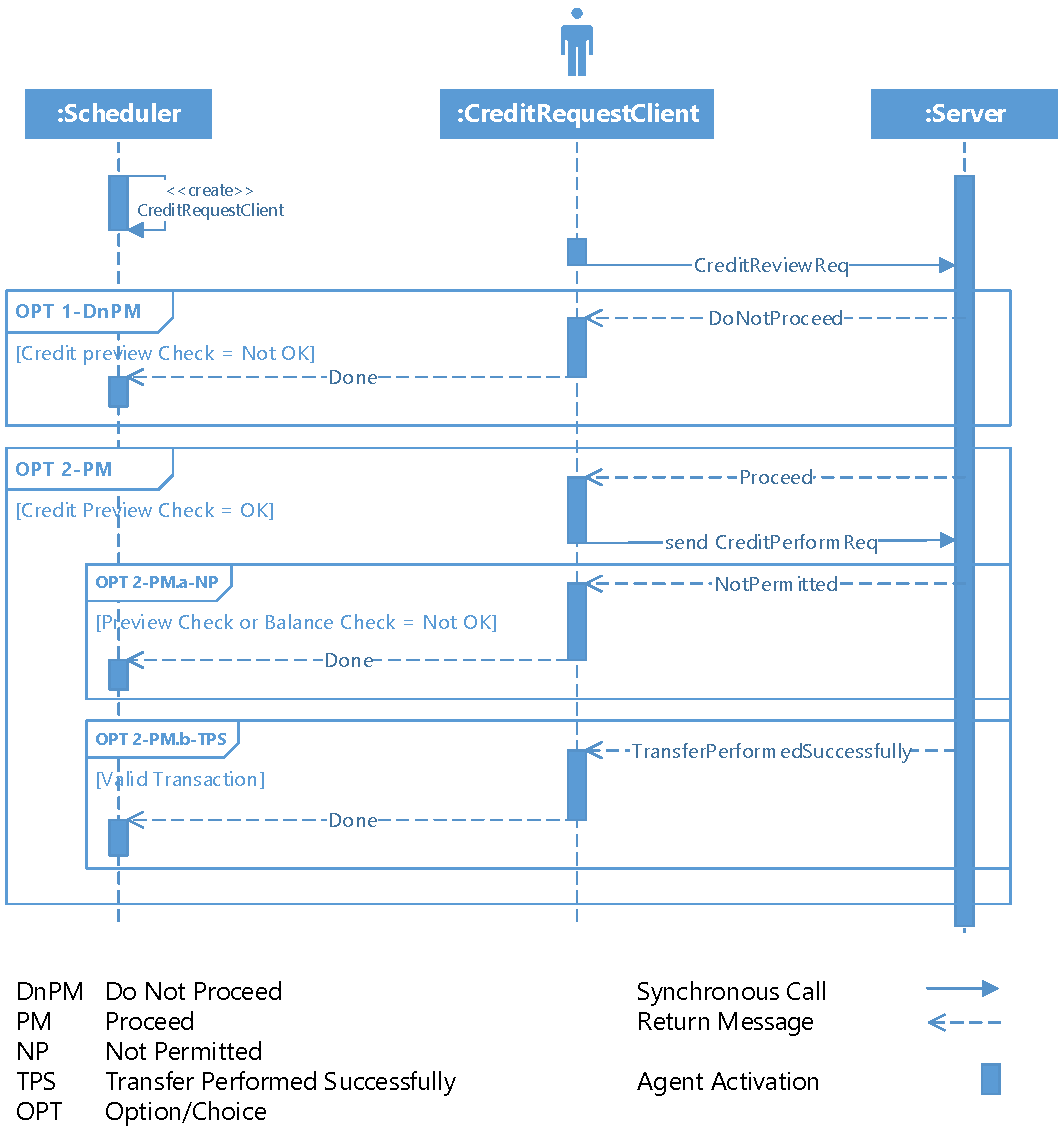
\includegraphics[width=1.0\textwidth]{Figures/creditrequest}
  \caption{\bf\small Credit request message protocol}
  \label{fig:impl-msg-crc}
\end{figure}

When following the sequence diagram in \ref{fig:impl-msg-crc} it is necessary to keep in mind that these messages are send from a $CreditRequestClient$ but initiated and owned by a member which is logged in and registered in the session data lookup table. For the server agent process it is important know which member is currently sending that transfer in order to perform various checks and store valid transfers. Certainly, same applies for the $DebitRequestClient$ and the $DebitAcknowledgeClient$ of figure \ref{fig:impl-msg-drc}.

\textbf{Dynamic Request Clients} start off when being created by the $scheduler$ agent and don't send or receive any request beforehand. According to a typical state machine the clients manage their own states and acting along them. CRC\footnote{Credit Request Client} and DRC \footnote{Debit Request Client} are using four main states which are explained in detail in \ref{subsec:impl-states}.

The message sequence from client to server is specified in \ref{fig:impl-msg-crc} for the CRC-client and in \ref{fig:impl-msg-drc} for the DRC-client. When investigating those two figures it is standing out that the message sequence looks very similar, only the names vary by their prefix (debit versus credit). However, what might not be obvious here is that the request parameters are quite different.

Another main difference between credit and debit message sequence is though, that a debit request needs $ConfirmationReq$ as well as $DebitAckMsg$. This is necessary because a initiating creditor (seller) needs to have the transaction confirmed by the debtor (buyer) to be sure having a valid transaction which is crediting the payment to the sellers own account.

\begin{figure}[htbp]
  \centering
  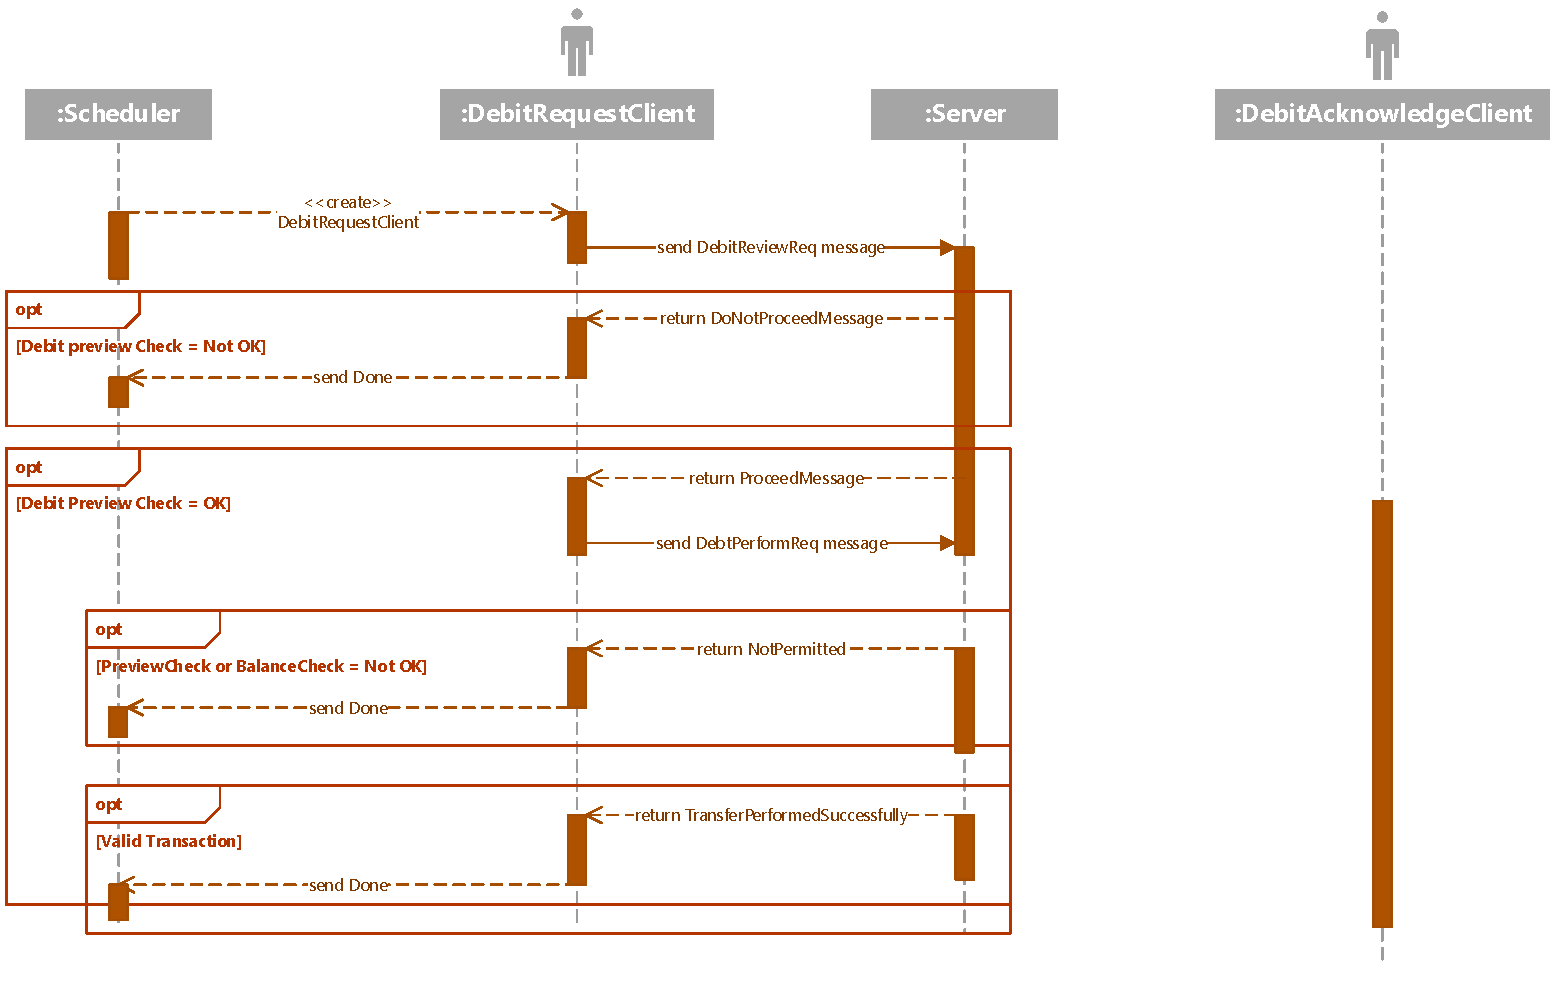
\includegraphics[width=1.0\textwidth]{Figures/debitrequest}
  \caption{\bf\small Debit request message protocol}
  \label{fig:impl-msg-drc}
\end{figure}

The sequence diagrams denote optional flows using option boxes. These boxes are having a unique numbered name. An option $OPT$ at the first level has a number (choice $1$ or $2$) as well as an abbreviated name ($DnPM$, $PM$). Sub-options in the second level are alphabetically numbered and also followed by an abbreviated name. Squared brackets underneath the option name indicate the current option choice.

ASIMs currently do not have the possibility to sleep for some time or until an event has occurred. Nevertheless, agents are able to reduce the executed command in the current tick to a minimum achieving a similar result. Inside of the sequence diagrams activated clients are shown by the vertical fully colored bars. Non-active phases are indicated by the vertical dashed lines.

The emulated users in the figures are pictured on top of the clients to show that request are send by particular member.

Scheduler and server are agents which can be seen as autonomous processes in the simulation. The scheduler mainly acts as an orchestration tool for testing purposes and will be removed for actually deployed applications whereas the server agent needs to exist in a real-world scenario. Maybe not as a process running on a centralized server structure but when taking a real distributed scenario into account it'll be implemented using some kind of smart contract running inside of a virtual machine in a blockchain-environment.

\subsection{State Management}
\label{subsec:impl-states}

\subsubsection{Client States}\ are managed over four predefined pseudo-static locations which are as following

\begin{itemize}
	\item SEND: only sending message
	\item RECEIVE: receive and directly respond to messages
	\item TERMINATE: end execution; send "Done" message
	\item DONE: everything is done; ready to be terminated
\end{itemize}

$SEND$ might be used if a sequence of messages will be sent were no replay message is needed or just to submit an initial message at start-up before going right into the $RECEIVE$-mode.

$RECEIVE$ waits for the messages and act accordingly. When a message has been received and it is necessary to send a response it is done right in $RECEIVE$-mode without changing to $SEND$-mode.

$SEND$ and $RECEIVE$ state could be set alternately but when state $TERMINATE$ is applied the process of shutting down the agent has been started. Once $DONE$-state is reached, even if not stopped yet by the scheduler, the client won't do anything useful any more.

The DAC\footnote{Debit Acknowledge Client} uses the same states except for the $SEND$-state because it only needs to receive and confirm a transfer by using the given one time pad. The DAC is an example that not all of the states need to covered by a client which might be of interest when creating new clients.

\subsubsection{Server \& Scheduler States}\ are not particular part of that section which is mainly about the dynamic clients, nevertheless, a brief explanation of their states is given here to keep them together.

\textbf{The server} does not have any particular mode or state management yet. It is just waiting for messages and when receiving one it will be directly processed.

\textbf{The scheduler} mainly has its test states as mentioned in  subsection \ref{subsec:impl-agent-tasks} and is transitioning from one test to another till there are no tests left. For each test the scheduler has two stages.

\textbf{First} in a starting phase all clients of that particular test are started and counted. Clients which should be part of one test state need to be defined as a dynamic client and appended to the scheduler by using the $include$-statement in the $run.icef$ definition.

Then the scheduler in its \textbf{second} phase waits for as many $DONE$-messages like clients have been issued. Finally, when the client count is zero, the scheduler goes to the next test and starts that two-phase process again.

%%%%%%%%%%TODO%%%%%%%%%
\section{Logging}
\label{sec:impl-log}

The server agent needs to place many different status messages of different importance. In order to manage their occurrence a simple logger has been added. The logger introduces five log levels:

\begin{enumerate}
	\item FATAL
	\item ERROR
	\item WARN
	\item INFO
	\item DEBUG
\end{enumerate}

Those levels denote different severities which can be applied to the logger and defines the maximum severity of a message presented to the executing user. To explain further $FATAL$ messages should be printed always whereas $DEBUG$ messages are only of interest for developers who need very detailed information of the current state.

Consequently, the maximum log level can be given at agent start-up inside of the $init$ rule. The rule used to define the level is explained here

\begin{lstlisting}[language=bsl]
	//rule header
	rule initCustomLogger(set_log_level) = ...
	...
	//init logger call
	initCustomLogger(DEBUG)
\end{lstlisting}

When initialized the logger can be used at any place by calling the $do\_log$-rule which is taking two parameters. The first is the actual the message printed to the output and the second parameter is describing the importance of that message by using one of the five mentioned severity levels. The listing beneath shows first how to log a message with severity $INFO$ and the second call illustrates a $FATAL$ error message output.
	
\begin{lstlisting}[language=bsl]
	// A "INFO"-level message
	do_log("Transfer has been performed successful", INFO)
	...
	// A "FATAL"-level error message
	do_log("List 'Leger' in unknown state", FATAL)
\end{lstlisting}

Currently the logger implementation can only be applied meaningful inside of the server itself, because the implementation is also hosted by the server agent definition file $server.casim$ directly. Certainly, it would be possible to put the logger into a different file but the $include$ statement of the $run.icef$ is not supported by the Eclipse Plug-in. Consequently, if the logger implementation would be separated out into an additional file all occurrences of $do\_log$ calls would be marked as erroneous (although they are not) and would then turn the coding-assistance-tools inside of Eclipse into an unusable environment.


\section{Test Scenario}
\label{sec:impl-test}

This deliverable is not covering the test management for the ICEF implementation of Interlace. However, in order to check if a base workflow of a requirement is working in its most simple form a strategy has been followed which has been partly explained already by other sections of chapter \ref{ch:CoreAsimImplementation}. The scope of this section will be therefore to put those parts together and extend the missing bits.

\subsection{Separation of Concerns}

When looking at the environment from a testing perspective there are three parts which can be distinguished. 

\begin{enumerate}
	\item Actual system requirements implementations
	\item Testing routines
	\item Simulation environment
\end{enumerate}

The "actual system requirement implementations" mentioned first cover parts which are needed for a possible real-world system. Without those the system would not be able to function and can be seen as the core part of the application which is entitled to be tested.

Second, code parts have been implemented which are only there for performing and validating a test of a particular scenario use case. Currently those scenarios are credit and debit operation requests sent from virtual clients.

Last, parts of the system had to be implemented prototypical and in their most basic form in order to receive a very simple executable version which can accommodate the test scenarios. Those parts were not included by the requirements definitions nor by the refinements. These parts comprise implementation details not relevant to the requirements as well as the main ledger implementation.

In \ref{subsec:impl-agent-tasks} the main agents are explained which are a $scheduler$ and a $server$. Those two, when assembled for execution, are containing all implementations. The $server$ covers the actual system requirement realizations and as well simulation environment code. To be more specific the $server$ is dispatching message request explained in \ref{lst:impl-msg-dispatch} and is performing read actions to virtual profile, account, etc. information together with pushing transactions to a primitive ledger shown in \ref{subsec:impl-sim-env}.

The $scheduler$ mostly contains testing routines but partly also routines handling necessary client implementations which are not covered by the requirements. The test routines are responsible for starting and destroying clients. As a short reminder, the $scheduler$ is able to do so because it also contains all the client code. Further, listing \ref{lst:impl-msg-send} shows the sending of a test credit request issued by the $CreditRequestClient$. This message is processed by a challenge-respond sequence between the server and the client imitating a transaction.

Concluding, a correct execution is currently only shown by a client which outputs a transfer-performed message when done. In case of an error the client would provide a message indicating the cause.

\subsection{Simulation Environment}
\label{subsec:impl-sim-env}

The simulation environment created for enabling the core server parts to be executed and later be validated has an active and a passive part. The so called active part takes care about storing a transaction into the ledger and the passive part contains various pre-prepared locations which are needed to satisfy the different requirement constraints.

\subsubsection{Locations: }\ Beginning with the passive part the following locations have been defined inside of the non-functional client $initdata$ shown in listing \ref{lst:impl-sim-setup-locs}.

\begin{center}
\begin{minipage}{0.8\textwidth}
\small
\begin{lstlisting}[language=bsl_lst,caption={\bf\small Simulation Environment Locations},label={lst:impl-sim-setup-locs} ]
controlled TT: OPERATION * UNIT * USER_TYPE_GROUP -> SET
controlled AccT: OPERATION * UNIT * ACCOUNT_TYPES -> SET

controlled profileTable: MEMBER_ID -> MAP
controlled accountTable: ACCOUNT_ID -> MAP
controlled userGroupTable: MEMBER_ID -> USER_TYPE_GROUP
controlled sessionData: MAP
\end{lstlisting}
\end{minipage}
\end{center}

The two most important are the functional locations $TT$ and $AccT$. They are corresponding to the transfer type matching described in \ref{subsec:perm-trans-types} and the account connectivity mentioned in \ref{subsec:perm-acc-con} respectively.

$TT$ got predefined precisely in the requirement definitions and is described as a functional mapping

\begin{asm}
TT: Operation \times Currency \times Group \rightarrow \{G \mid G \subseteq Group\}
\end{asm}

So we can define for an Credit-Operation in Sardex (SRD) an $Employee$ is allowed to perform a transaction with a member of the circuit which is part of one of the groups $Company$, $Retail$ or $Full$:

\begin{asm}
TT^{Credit,SRD}(Employee) =\{Company,Retail,Full\}
\end{asm}

When translating this discrete functional mapping to BSL the outcome is looking like this

\begin{lstlisting}[language=bsl]
	TT("credit", "SRD", "employee") := {"company", "retail", "full"}
\end{lstlisting}

The account connectivity function $AccT$ is taking operation, currency and account type as parameters and is then mapping them to a group of account types

\begin{asm}
AccT: Operation \times Currency \times AccountType \rightarrow \{AccT \mid Acct \subseteq AccountType\}
\end{asm}

When replacing the parameters by actual values the following may be written down 

\begin{asm}
\begin{array}{ll}
AccT^{Credit,SRD}(X) =\{ CC , Domu ,Mirror \} & \IF X \in CC
\end{array}
\end{asm}

which then can be transformed again into the "implemented" form and is represented like this inside of the $initdata$ agent

\begin{lstlisting}[language=bsl]
	AccT("credit", "SRD", "CC") := {"CC", "DOMU", "MIRROR"}
\end{lstlisting}

The other location listed in listing \ref{subsec:perm-trans-types} are accommodating important information for groups, members, sessions as well as accounts. Except for the $userGroupTable$ which is just mapping a user to its current operational group all functions implementing a result type of $MAP$. A $MAP$ is similar to a simple set with the difference that each entry of a $MAP$ is a key-value pair.

\begin{center}
\begin{minipage}{0.8\textwidth}
\small
\begin{lstlisting}[language=bsl_lst,caption={\bf\small $MAP$ example showing a profile table entry},label={lst:impl-sim-maps} ]
	//init profile data
	profileTable("mbrId1") := {
		"lowBalanceAlert" -> 700,
		"highBalanceAlert" -> 1000,		
		"highVolumeAlert" -> 10000,
		"capacity" -> 100000,
		"saleVolume" -> 50000,
		"accounts" -> ["accId1", "accId4"]
	}
\end{lstlisting}
\end{minipage}
\end{center}

Listing \ref{lst:impl-sim-maps} shows a typical definition of such a map which may be compared to a hash map used in various different other programming languages. Those values are accessed based on different pre-defined rules which are explained in section \ref{sec:impl-rules}.

\subsubsection{Ledger: }\ The ledger but also the pending transactions are initialized as empty maps

\begin{lstlisting}[language=bsl]
	Ledger := {->}
	PendingTransactions := {->}
\end{lstlisting}

and when a transaction is matching the required constraints it is appended to that ledger map. For unconfirmed debit requests an second map called $PendingTransactions$ has been added which contains valid transactions which have not yet been confirmed by the debtor yet.

After the various checks which vary a little based to the type of operation have been successful the transaction is appended using the following command 

\begin{lstlisting}[language=bsl]
	Append(Transaction(transfer, client, "debit", now), Ledger)
\end{lstlisting}

A pending transaction awaiting a correct OTP from a debtor are added to location $PendingTransactions$ like this

\begin{lstlisting}[language=bsl]
	Insert(transfer, creditor, PendingTransactions) Ledger)
\end{lstlisting}

After a transaction got confirmed by a valid OTP it is moved, as mentioned, to the actual ledger. Inside of the the $PendingTransactions$ map that transactions receives state $TRANSACTION\_PERFORMED$ but will not be deleted.

\subsection{Additional Login Layer}
\label{subsec:impl-login-layer}

The requirements definitions do not define how authentication is handled on the system. Agents in ICEF have predefined names which cannot be changes during runtime. In order to act flexible and reuse agents a login layer has been introduced. Thus agents who are actively communicating with the server need to be registered inside of the $sessionData$ location which is initialized in the $initdata$ function.

Agents on the current prototypical implementation do not login by themselves by providing a user name and password but by placing its address together with a valid member id inside of $sessionData$-MAP as shown here

\begin{lstlisting}[language=bsl]
	sessionData := {
		"CreditRequestClient@CreditRequestClient" -> "mbrId1",
		"DebitAcknowledgeClient@DebitAcknowledgeClient" -> "mbrId4",
		"DebitRequestClient@DebitRequestClient" -> "mbrId2"
	}
\end{lstlisting}

The address of an agent is defined by "<name>@<name>", thus concatenating its own name with an "@"-symbol. The address is taken during message processing to determine that f.e. agent "CreditRequestClient" messages are sent by user "mbrId1" when looking at the above $sessionData$ set-up.

The member-id is representing an alpha-numerical string assigned after first registration. For the Interlace implementation this means that an entry also needs to exist in location $profileTable$ as well as in $userGroupTable$, which means that the user has been properly registered and is known to the system. If a valid transaction should be placed an entry inside of location $accountTable$ for that user should be added to assign and work with an actual account.

During runtime two derived functions are used to read the information of $sessionData$. As shown beneath a member-id of an "active" user can be determined by calling $activeLogin$. To check if a member is currently logged-in may be found out by obtaining the result of $activeClient$.

\begin{lstlisting}[language=bsl]
	//get member id by providing a client name using session information
	derived activeLogin(client_address) = ...
	//usage
	login_mbrId := activeLogin("CreditRequestClient@CreditRequestClient")
	
	//get client name by providing member id using session information
	derived activeClient(login_mbrId) = ...
	//usage
	client_address := activeClient("mbrId1")
\end{lstlisting}

One restriction needs to be mentioned though. A client address only can have one member being logged-in at one time and vice versa.

\section{Important Rules and Locations}
\label{sec:impl-rules}

Next the emphasis is put on explaining rules and locations not discussed in detail or not mentioned at all in this document yet. All rules and locations in this section can be located inside of file $server.casim$ or $initdata.casim$ which is added to the server part due to the $include$-statement inside of run.icef.

In BSL-code you need to use the $choose$-keyword to read content inside a map which make code difficult to read in some cases. To simplify that access, a derived function $v$ got introduced for working with $MAP$-type locations:

\begin{lstlisting}[language=bsl,mathescape=true]
	$\Rightarrow$ derived v(amap, key)
\end{lstlisting}

The parameter $amap$ can be any $MAP$-type location and the $key$ refers to the entry of interest. Consequently, the corresponding $value$ can be read by passing an existing $key$ like illustrated in the following example

\begin{lstlisting}[language=bsl,mathescape=true]
	mymap := {
		"thekey" => "assignedvalue",
		"another" => "somevalue"		
	}
	valueofkey := v(mymap, "thekey")
\end{lstlisting}

Concluding further, if the map or the key is undefined, also the result will be.

The ICEF-framwork uses a Plug-in called "CommunicationPlugin" to establish a simple communication system. As mentioned in previous section a method called $send$ is used to transfer a message. However, the server implementation usually does not call that method directly but rather a rule with the same name starting with an upper-case letter. That $Send$ rule takes as first parameter a message which contains a list of two strings. Those two strings are the message content itself as well as the message subject. In order to abstract the message type from the user a derived rule called $AssembleMessage$ is provided for creating such a message. The second parameter is the recipient agent name, not a member with a particular id:

\begin{lstlisting}[language=bsl,mathescape=true]
	$\Rightarrow$ derived AssembleMessage(msg, sub)	
	$\Rightarrow$ rule Send(msg, agent)
\end{lstlisting}

When passing a message before sending, other parts of the implementation may use $messageContent$ and $messageSubject$ functions on the assembled message to get back the content and the subject respectively. Also $Send$ uses those two function to read content and subject for the actual sending process.
In case of error or success specific messages are created. $IncorrectOtpFor$ is one example which is used inside the $server$ implementation to create an appropriate error message based on particular related arguments:

\begin{lstlisting}[language=bsl,mathescape=true]
	$\Rightarrow$ derived messageContent(msg)
	$\Rightarrow$ derived messageSubject(msg)
	$\Rightarrow$ derived IncorrectOtpFor(otp, amount, creditor)
\end{lstlisting}

Continuing further on OTPs there are three important functions to mention on top of the requirement definitions. $RandomHex$ is generating a random hex-decimal number. Next $HexString$ calls $RandomHex$ $n$ times where $n$ equals the first parameter $length$ resulting in a hex-decimal string. That hex-decimal generation is used for creating one time passwords (OTPs) as well as transaction ids for appending unique transactions to the ledger.

\begin{lstlisting}[language=bsl,mathescape=true]
	$\Rightarrow$ derived RandomHex
	$\Rightarrow$ derived HexString(len)
	$\Rightarrow$ derived OneTimePassword(strength)
\end{lstlisting}

Transactions are transferred using a $MAP$. A credit transfer is shown next:

\begin{lstlisting}[language=bsl,mathescape=true]
	$\Rightarrow$ CREDITREQUEST := {
			"from" -> "accId1",
			"to" -> "accId2",
			"channel" -> "Service",
			"amount"  -> 2000,
			"metadata" -> {"message", "some transfer"}
	  }	
\end{lstlisting}

For all attributes used inside those transfer-request-maps derived functions have been created. One function and its usage is shown here:

\begin{lstlisting}[language=bsl,mathescape=true]
	$\Rightarrow$ derived fromAcc(transfer)
	// example
	fA := fromAcc(CREDITREQUEST)
	fA = "accId1" //is true
\end{lstlisting}

Next the focus is put on the ledger and the preliminary storage for pending transactions. Both are maps storing transactions. The difference is that $PendingTransactions$ are using an OTP-key to map to a transaction whereas a finally persisted transaction is mapped using an transaction-id-key. One time pads are created by $OneTimePassword$ and transaction ids are created by calling $NewTransactionID$.

\begin{lstlisting}[language=bsl,mathescape=true]
	$\Rightarrow$ controlled Ledger: MAP
	$\Rightarrow$ controlled PendingTransactions: MAP
\end{lstlisting}

Rule $Insert$ is adding a transaction which is awaiting confirmation to a map which needs to be the last parameter. The $server$ stores all those unconfirmed request inside of map PendingTransactions as indicated above.

After a valid and existing OTP has been sent for a transfer inside of $PendingTransactions$ the transfer needs to undergo some more checks, but when passed, it is appended to the Ledger by executing rule $Append$.

$Insert$ and $Append$ are listed here together with $Transactions$ and $NewTransactionID$:

\begin{lstlisting}[language=bsl,mathescape=true]
	$\Rightarrow$ rule Append(trans, ledger)
	$\Rightarrow$ rule Insert(transfer, creditor, pendingTransactions)
	$\Rightarrow$ derived NewTransactionID(len)
	$\Rightarrow$ derived Transaction(transfer, mbr, operation, date)
\end{lstlisting}

Finally a rule is described which is part of the requirements but used in a different way. The requirements are using three functions called $FinalDebitAccountLimitsCheck$, $DebitAccountLimitsCheck$, $CreditAccountLimitsCheck$. Those function are basically similar and used in a consolidated way for the ICEF-implementation. $PrevieCheck$ implements that check and needs the member id $mbr$, the from account $fromA$, the to account $toA$, a from group $fromGroupId$, a $toGroupId$ and as last parameter the operation $operation$ as string. The operation string can be either "credit" or "debit". This code example is showing the rule but also how it is used in the current set-up:

\begin{lstlisting}[language=bsl,mathescape=true]
	$\Rightarrow$ rule PreviewCheck(mbr, fromA, toA, fromGrpId, toGrpId, operation)
	//example: do check the transfer if it is ok
	error <- PreviewCheck(
		activeLogin(client), //read mbr from message client-address
		fromAcc(transfer), //read from account of transfer
		toAcc(transfer), //read to-account of transfer
		groupOf(ownerOf(fromAcc(transfer))), //get group of from-account owner
		groupOf(ownerOf(toAcc(transfer))), //get group of to-account owner
		"credit" //Operation as string
\end{lstlisting}

The result of $PreviewCheck$ is either $undef$ in case all checks are successful or are containing a message text indicating the problem.

\section{Implementation Challenges}
\label{sec:impl-challenges}

When working with the ICEF-framework some thing need to be noted. Currently, the ICEF-framework is an academic tool and not ready for professional usage. Some efforts need to be applied in order to achieve a fully integratable system for a software design process or even a continuous integration process.

\subsection{Issues}

During development the team has been confronted with different issues regarding the ICEF-framework but also with the process moving the specifications to a running ASIM Interlace Model. Next the issues are listed and explained:

\begin{description}
	\item[Unknown line numbers] Before transmitting a simulation to the ICEF manager JavaScript code is loading all specified casim files preparing them for being sent over the network in form of a consolidated JSON-message. That process together with the added preliminary $include$-syntax are causing a problem for error message. More precisely that they do not contain appropriate line numbers if something goes wrong. Thus in case of any failure it is sometime very hard to locate the actual cause.
	\item[Error in block] Errors inside of a block are causing the whole block not being executed for unknown cases. So, if a block has n-statements and the last one has a problem all the other n-1 might not be executed as well. Even if a sequential block has been used. Given that the error messages do not contain correct line numbers finding a problem with debug output to the console also does not work appropriately in all of the cases.
	\item[Parallel blocks] ASM code and consequently also BSL code allows to write so-called parallel blocks. Those blocks start with $par$, end with $endpar$ and contain code which is executed in parallel - at least theoretical. The important thing to know here is that the order of execution is not guaranteed. This can lead and actually leaded during development to unpredictable behaviour and needs to be used with caution!
	\item[Bugs] As the ICEF framework is still in an alpha version state couple of bugs occurred which could be fixed. However, there are further iterations needed to make the framework stable.
	\item[Testing] Various testing approaches still need to be investigated, because at the moment only the text output of a simulation can be checked to test if the system is running correct. These testing approaches will be part of the upcoming research.
	\item[Modules] The solution of how modules or how other code snippets are integrated comes with strings attached like the mentioned inaccurate line numbers and duplicate name spaces. Thus a re-factoring for later use is highly recommended.
	\item[From document based to executable] When a system behaviour has been written down in form of an ASM specification it is necessary to note that a direct translation to ASM/BSL code is not always straight forward. One reason is that the functions and rules are not consistently available for coreAS(I)M as well as a lot of code for "getting it to run" needs to be worked out.
\end{description}

\subsection{Current Status}

The requirements for credit and debit operations have been implemented and are ready for more sophisticated tests. Also the base conditions for including further operations or requests handled by the server can be easily extended.

A test scenario has been build which may be used later for high level testing where particular use cases are played through using a predefined set of tests including agents with particular tests.

Nevertheless, B2C-operations and also some of the other requests defined like $AccountHistReq$ still need to be taken care of.
\chapter{Outlook and Next Steps}
\label{ch:Outlook}

\vspace{-1cm}
\begin{center}
Paolo Dini and Eduard Hirsch
\end{center}

This report has provided an update on the business logic requirements of the next-generation mutual credit transactional platform, relative to currently available technology (Chapter \ref{ch:UpdatedBLS}). It has provided a detailed explanation of the configuration and setup of the ICEF executable modelling framework for ASIMs and of its implementation language CoreASIM (Chapter \ref{ch:CoreAsimIntro}). In the Appendix, it provided a formalization of the updated requirements. Finally, in Chapter \ref{ch:CoreAsimImplementation} it presented a detailed discussion of the CoreASIM implementation of the specification shown in the Appendix.

The business logic requirements of Chapter \ref{ch:UpdatedBLS} represent an intermediate step between the current centralized system being used by SARDEX and based on a relational database and the blockchain-based platform INTERLACE is tasked with developing. Such an intermediate step is needed both from the point of view of engineering robustness, since migrating to a new platform is difficult and risky, as well as because the the full functionality of the blockchain platform will depend to some extent on the technology features of the framework employed.

The implementation of the business logic as an executable CoreASIM model has also had the added benefit to bring into focus the need for a testing framework for the ICEF, which is currently missing. In the short term, this can be provided by manually composed testing scenarios written in Gherkin\footnote{\url{https://docs.cucumber.io/gherkin/}} and Cucumber,\footnote{\url{https://cucumber.io/}}since they are used by the Hyperledger blockchain development community. In the long term, it would be helpful to develop a ``compiler'' from the ASIM specification directly into Gherkin.

The next step for INTERLACE will be to specify, model (D2.2), and implement (D3.2) a blockchain platform that supports at least part of the business logic presented in this report. We have decided to use Hyperledger Fabric as the most suitable framework for the needs of INTERLACE and of the Sardex circuit. In other words, we will develop a permissioned blockchain with a limited number of nodes. However, the great flexibility and customizability of Hyperledger leaves open the possibility of coupling the permissioned blockchain to a public permissionless blockchain at some point in the future. Whereas this is not likely to be needed for mutual credit transactions within a single circuit, it could be useful to support scalability features for inter-circuit trade.












%\input{2-DLTs_Selected/dlt}
%\input{3-Functional_Requirements/funreq}
\chapter*{References}
\renewcommand{\section}[2]{}

\setlength{\parskip}{0.8\baselineskip}
\bibliographystyle{plainurl}
\small
\addcontentsline{toc}{chapter}{References}
\bibliography{Bib/BioComp_References}

%===================================================
%================== APPENDIX
%===================================================
%\begin{appendix}
%\section*{Appendix}
%\includepdf[pages={-}]{sections/4-CaSM/CaCycleAsm.pdf}
%\end{appendix}

\end{document}
